%% Placeholder for chapter on vector and functions

\noindent\textcircled{1} Geometry\\
-Vectors and vector spaces\\
-Norms\\
-Inner product\\

\noindent\textcircled{2} Projection\\
-Onto subspace\\
-Onto affine sets\\
-Non-Euclidean\\

\noindent\textcircled{3} Functions\\
-Functions and sets\\
-Linear and affine\\
-Gradients and Taylor approximations\\

\newpage

\noindent\textbf{Vector}: A collection of numbers.
\begin{equation*}
x = \left[ \begin{array}{c} x_1 \\ x_2 \\ \vdots \\ x_n\end{array} \right].
\end{equation*}
where each $x_i \in \reals$ or $x_i \in \complex$. The length $n$ of the vector is also termed as the "dimension" of the vector, which will subsequently be defined formally.

Our default will be a column vector as we describe above. Transpose $x$ yields a row vector,   
\begin{equation*}
x^\trans = [ x_1 \ x_2 \ \ldots x_n].
\end{equation*}
and occasionally write as a list $(x_{1}, x_{2},\cdots,x_{n})$.  Note that a vector is not a set of numbers since order matters.

Also, we often need to work with a set(or list) of vectors,
\begin{equation*}
\{ \vecx{1}, \vecx{2}, \ldots, \vecx{m}\}
\end{equation*}
where $\vecx{i} \in \reals^n$, $i \in \{1, 2, \ldots, m\}$, $i \in [m] = \{1,2,\cdots,m\}$ and
$(\vecx{i})^\trans = [ \vecx[1]{i} \ \vecx[2]{i} \ \ldots \ \vecx[n]{i} ]$.  

Note: The textbook is not 100\% consistent in its use of this notation.

\vspace{0.5cm}
\noindent\textbf{Vector Space}

First, we define how to add pairs of vectors and how to scale vectors as follows:

Addition: $u=v^{1}+v^{2}$, means $u_{i}=v_{i}^{1}+v_{i}^{2}$ for all $i\in [n]$.

Scaling: $u=av$,  means $u_{i}=v_{i}^{1}+v_{i}^{2}$ for all $i\in [n]$.

Linear combination: $\sum_{i=1}^{m} a_{i}v^{(i)}$

\begin{marginfigure}
	\centering
	\resizebox{7.5cm}{3cm}{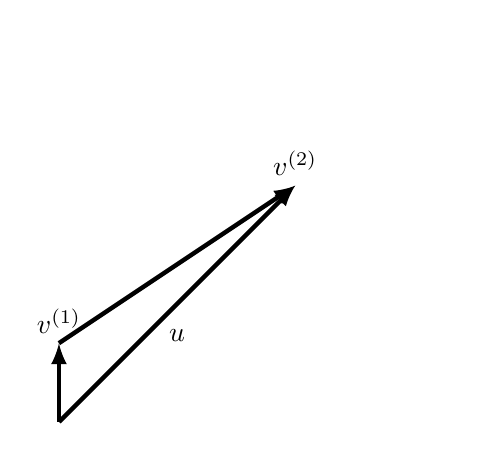
\begin{tikzpicture}
\draw [white, <->] (0,5) -- (0,0) -- (5,0);
\draw [-latex, ultra thick] (0,0) -- (0,1);
\draw [-latex, ultra thick] (0,0) -- (3,3);
\draw [-latex, ultra thick] (0,1) -- (3,3);
\node [above] at (0,1) {$v^{(1)}$};
\node [below] at (1.5,1.3) {$u$};
\node [above] at (3,3) {$v^{(2)}$};
\end{tikzpicture}}
	\caption{Addition}
	\label{fig.2-1}
\end{marginfigure}
\begin{marginfigure}
	\centering
	\resizebox{7.5cm}{3cm}{\begin{tikzpicture}
\draw [white, <->] (0,5) -- (0,0) -- (5,0);
\draw [-latex, ultra thick] (0,0) -- (1.5,1.5);
\draw [-latex, ultra thick] (1.5,1.5) -- (3,3);
\node [above] at (0.75,0.75) {$v^{(1)}$};
\node [above] at (3,3) {$u=2v^{(1)}$};
\end{tikzpicture}}
	\caption{Scaling}
	\label{fig.2-2}
\end{marginfigure}

\vspace{0.5cm}

\textbf{Vector Space}: a set of vectors $v$ that is closed under addition and scaling, and satisfy following axioms:

(1) Commutativity: $u+v=v+u$

(2 )Associativity: $(u+v)+w=u+(v+w)$

(3) Distributivity: $a(u+v)=au+av$,\ $(a+b)u=au+bu$

(4) Identity element of addition: $\exists 0\in \cal{V}$ s.t. $u+0=u$

(5) Inverse elements of addition: $\exists -u\in \cal{V}$ s.t. $u+(-u)=0$

(6) Identity element of scalar multiplication: $\exists a\in \reals\ \text{or}\ \complex$ s.t. $au=u$

\vspace{0.5cm}
In this course our focus is on $\reals^{n}$, i.e., finite-length vectors with real elements. It is also useful to note that the geometric ideas could apply to lots of other spaces, such as

\textcircled{1} Finite-length complex vector\\
we need this especially for discussion of eigenvalues and eigenvectors. But it is also important example in quantum computing.\\
\textcircled{2} $\infty$-length complex sequences\\
\textcircled{3} Complex functions defined on real line\\
\textcircled{4} Polynomials of degree at most n-1\\
$$P_{n-1}=\{P|p(t)=a_{n-1}t^{n-1}+a_{n-2}t^{n-2}+\cdots + a_{1}t+a_{0} \}$$

\textcircled{5} Sets of matrices(will discuss later)\\
\vspace{0.3cm}
Note: Some authors prefer “linear space" rather than "vector space" since elements of space are not always vectors in the sense of a list.

\vspace{0.5cm}

\textbf{Span and subspace}

Let $S$ be a set of vectors in a real vector space $V$, i.e.,$S=\{v^{(1)}, v^{(2)}, \ldots ,v^{(m)}\}$, where each $v^{(i)}\in \reals^{n}$. Then, the span of $S$, denoted by span($S$), is the set consisting of all the vectors that are linear combinations of $\{v^{(1)}, v^{(2)}, \cdots ,v^{(m)}\}$, that is, 
$$\text{span}(S)=\left\{\sum_{i=1}^{m} a_{i}v^{(i)}\middle| a_{i}\in \reals ,\forall i\in [m]\right\}$$

This set is also called a \textbf{subspace} of $V$.

\vspace{0.3cm}
Example 1

\begin{marginfigure}
	\centering
	\resizebox{7.5cm}{3cm}{\begin{tikzpicture}
\draw [white, <->] (0,3) -- (0,0) -- (3,0);
\draw [-latex, ultra thick] (0,0) -- (1,1);
\draw [dashed,ultra thick] (-2,-2) -- (2,2);
\node [below right] at (0,0) {(0,0)};
\node [above left] at (1,1) {$v^{(1)}$};
\end{tikzpicture}}
	\caption{Example 1}
	\label{fig.2-3}
\end{marginfigure}

\begin{marginfigure}
	\centering
	\resizebox{7.5cm}{3cm}{\begin{tikzpicture}
\draw [<->] (0,4) -- (0,0) -- (4,0);
\draw [->] (0,0) -- (3,2);
\draw [dashed] (0,0) -- (-1.5,-1);
\draw [-latex, ultra thick] (0,0) -- (1.7,0.5);
\draw [-latex,ultra thick] (0,0) -- (0.8,-1);
\node [below] at (4,0) {x};
\node [below] at (3,2) {y};
\node [left] at (0,4) {z};
\node [above right] at (1.7,0.5) {$v^{(1)}$};
\node [below left] at (0.8,-1) {$v^{(2)}$};
\end{tikzpicture}}
	\caption{Example 2}
	\label{fig.2-4}
\end{marginfigure}

Let $S=\{v^{(1)}\}=\left\{ 
\left[ 
\begin{array}{c} 
1 \\
1
\end{array}
\right]\right\}$, then
\begin{align*}
\text{span}(S)&=\text{span}({v^{(1)}})\\
&=\left\{\left[ 
	\begin{array}{c} 
	x \\
	y
	\end{array}
	\right]\middle|x=y\right\}\\
&=\left\{a\left[ 
	\begin{array}{c} 
	1 \\
	1
	\end{array}
	\right]\middle|a\in\reals\right\}
\end{align*}\\

Example 2\\
Let $S=\{v^{(1)}, v^{(2)}\}=\left\{\left[ 
\begin{array}{c} 
1\\
1\\
0
\end{array}
\right],           
\left[ 
\begin{array}{c} 
1\\
-1\\
0
\end{array}
\right]
\right\}$, then

\begin{align*}
\text{span}(S)&=\{a_{1}v^{(1)}, a_{2}v^{(2)}|(a_{1}, a_{2})\in \reals^{2}\}\\
&=\left\{\left[ 
	\begin{array}{c} 
	x\\
	y\\
	0
	\end{array}
	\right] \middle|x\in\reals , y\in\reals\right\}\\
&=\text{$x-y$ plane}
\end{align*}\\


Note:

(1) $0\in\reals^{n}$ always included since we can set all coefficients $a_{i}=0$ for all $i$.

(2) Subspace is a "flat" that goes through the origin.

\vspace{0.5cm}
\noindent\textbf{Linear independent set}

A set $S=\{v^{(1)},\cdots , v^{(n)}\}$ is a linearly independent set if there is no element of $S$ can be expressed as a linear combination of the others.

The set $S$ is linearly independent if the only if $a_{i}$ that satisfies
$$\sum_{i=1}^{m}a_{i}v^{(i)}=0\quad \text{is if} \quad a_{i}=0 \ \forall i\in [m]$$


\vspace{0.5cm}
\textbf{Importance of linearly independent}

For any $u\in \text{span}(S)$ , there is a unique linear combination to express $u$. That is, only one choice of $a_{i}$ in the expression.

\begin{marginfigure}
	\centering
	\resizebox{7.5cm}{3cm}{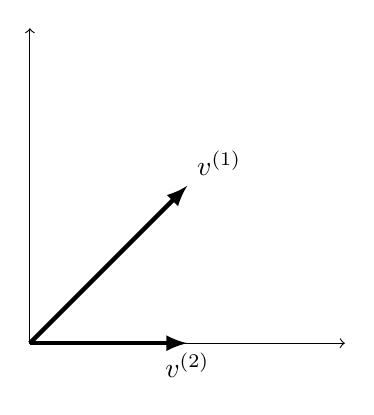
\begin{tikzpicture}
\draw [<->] (0,4) -- (0,0) -- (4,0);
\draw [-latex, ultra thick] (0,0) -- (2,2);
\draw [-latex,ultra thick] (0,0) -- (2,0);
\node [above right] at (2,2) {$v^{(1)}$};
\node [below] at (2,0) {$v^{(2)}$};
\end{tikzpicture}}
	\caption{}
	\label{fig.2-4}
\end{marginfigure}
\begin{marginfigure}
	\centering
	\resizebox{7.5cm}{3cm}{\begin{tikzpicture}
\draw [<->] (0,5) -- (0,0) -- (5,0);
\draw [-latex, ultra thick] (0,0) -- (2,2);
\draw [-latex,ultra thick] (2,2) -- (4,2);
\draw [dashed,ultra thick] (-2,2) -- (5,2);
\node [below] at (5,0) {$u_{1}$};
\node [left] at (0,5) {$u_{2}$};
\node [above right] at (4,2) {$a_{1}v^{(1)}$};
\node [below right] at (2,2) {$a_{2}v^{(2)}$};
\end{tikzpicture}}
	\caption{}
	\label{fig.2-4}
\end{marginfigure}


\vspace{0.5cm}
For example, any 2-d vector $u$ can be uniquely expressed by the following two vectors $v^{(1)}$ and $v^{(2)}$, which form the set $S$. 
$$v^{(1)}= 
\left[ 
\begin{array}{c} 
1 \\
0
\end{array}
\right]
,
v^{(2)}= 
\left[ 
\begin{array}{c} 
1 \\
1
\end{array}
\right]$$


Notice that the two vectors are co-linear so that there is no redundancy in the set $S$. Now, consider the case there is a redundancy in $S$, i.e., there is a vector in $S$ can be expressed by the others in $S$:


$$S=\left\{\left[ 
\begin{array}{c} 
1\\
0
\end{array}
\right],           
\left[ 
\begin{array}{c} 
1\\
1
\end{array}
\right],
\left[ 
\begin{array}{c} 
0\\
1
\end{array}
\right]
\right\}$$

We can prove that we can always shrink $S$ by removing elements to get a linearly independent set(and also the same subspace before the deletion). Such an irreducible or linearly independent set can serve as a \textbf{basis} for span($S$).

Any largest linearly independent subset of $S=\{v^{(1)},\cdots , v^{(m)}\}$, $B=\{v^{(1)},\cdots , v^{(k)}\}$, $k\leq m$ is a basis for span($S$), and the dimension of span($S$) is denoted as  dim(span($S$))=$k$.

\vspace{0.5cm}
Example 1

The following vectors form an linearly independent spanning set $S$, and also serve as a basis for the vector space spanned by the set $S$ (i.e., $\reals^{3}$ in this case)

$$v^{(1)}= 
\left[ 
\begin{array}{c} 
1 \\
1 \\
1
\end{array}
\right],
v^{(2)}= 
\left[ 
\begin{array}{c} 
1 \\
2 \\
0
\end{array}
\right],
v^{(3)}= 
\left[ 
\begin{array}{c} 
1 \\
3 \\
1
\end{array}
\right]$$


However, if we redefine $v^{3}$, says
$$v^{(3)}= 
\left[ 
\begin{array}{c} 
3 \\
4 \\
2
\end{array}
\right]
=2v^{(1)}+v^{(2)}$$

Then $\left(v^{(1)},v^{(2)}, v^{(3)}\right)$ is not a basis(since it is linearly dependent now), and it need to be reduced to:
$$\text{span}\left(\{v^{(1)},v^{(2)}\}\right)=\text{span}\left(\{v^{(1)},v^{(3)}\}\right)=\text{span}\left(\{v^{(2)},v^{(3)}\}\right)=\text{span}(S)$$

We can prove that each a basis for span($S$) all have same coordinates.

\vspace{0.3cm}
Example 2

The most commonly used basis is the "standard" basis, that is, each vector of the basis has a unit length:
$$v^{(1)}= 
\left[ 
\begin{array}{c} 
1 \\
0 \\
0 \\
\vdots
\end{array}
\right],
v^{(2)}= 
\left[ 
\begin{array}{c} 
0 \\
1 \\
0 \\
\vdots
\end{array}
\right], \cdots,
v^{(n)}= 
\left[ 
\begin{array}{c} 
0 \\
0 \\
\vdots \\
1 
\end{array}
\right]$$

We often use $'e'$ for standard basis, i.e., $e^{(i)}=v^{(i)}$.

\vspace{0.5cm}
\noindent\textbf{Norms}: The idea of distance on length on a vector space $\cal{V}$

A norm $\Vert\cdot\Vert$ is a function such that $\Vert\cdot\Vert : \cal{V}\mapsto\reals$
and satisfies

(a) $\Vert v \Vert\geq 0$, $\forall v\in \nu$, and $\Vert v \Vert=0$ iff $v=0$.

(b) $\Vert u+v \Vert\leq \Vert u \Vert+\Vert v \Vert$, $\forall u, v\in \cal{V}$.

(c) $\Vert au \Vert= \vert a\vert\Vert u \Vert$, $\forall a\in\reals, u\in\cal{V}$

Note that $\nu$ can be either $\reals$ or $\complex$, if $\cal{V}\in\complex$ we should have $a\in\complex$ in (c).

\vspace{0.5cm}
Following is a family of norms that are frequently used:

$L_{p}$ norm:
$$\Vert x\Vert_{p}=(\sum_{k=1}^{n}\vert x_{k}\vert^{p})^{1/p}, 1\leq p\leq\infty$$

$L_{2}$ norm: Euclidean length
$$\Vert x\Vert_{2}=\sqrt{\sum_{k=1}^{n}\vert x_{k}\vert^{2}}$$

$L_{1}$ norm:
$$\Vert x\Vert_{1}=\sum_{k=1}^{n}\vert x_{k}\vert$$

$L_{\infty}$ norm:
$$\Vert x\Vert_{\infty}=\lim_{p\to\infty}\Vert x_{k}\Vert_{p}=\max_{k\in [n]} \vert x_{k}\vert$$

\vspace{0.5cm}
Length is a notion of "size". A natural notion of its "size" of a set is the number of non zero component, i.e., carnality of non-zero support
$$\text{card}(x)=\sum_{k=1}^{n}\mathbb{1}_{x_{k}\neq 0}$$

Sometimes it is called "$L_{0}$" norm $\Vert x\Vert_{0}$, since $\text{card}(x)=\lim_{p\to 0}(\sum_{k=1}^{n}\vert x_{k}\vert^{p})^{p}$, but it is not a norm (so this terminology is inaccurate). For instance, it doesn't satisfy property (c) of a norm:
$$\text{card}(2x)=\text{card}(x)\neq 2\text{card}(x)$$

\textbf{Unit norm-ball}

To visualize a norm we often plot the unit norm-ball $\beta_{p}=\{x|\Vert x\Vert_{p}\leq 1\}$ in $\reals^{2}$. For example,

\vspace{0.3cm}
$L_{2}$ norm ball

\begin{figure}
	\centering
	\resizebox{7.5cm}{3cm}{%% page 15
%% fig 1
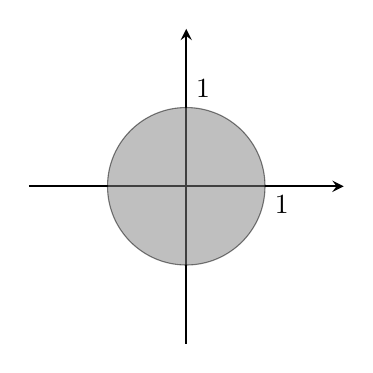
\begin{tikzpicture}
\draw[thick,-stealth] (-2, 0) -- (2, 0);
\draw[thick,-stealth] (0, -2) -- (0, 2);

\filldraw[fill=gray, draw=black, opacity=0.5] (0,0) circle [radius=1];
\node [below right] at (1, 0) {1};
\node [above right] at (0, 1) {1};
\end{tikzpicture}}
%	\caption{$L_{1}$ norm ball}
	\label{}
\end{figure}

$L_{1}$ norm ball : $\{x|\vert x_{1}\vert\leq 1\}$

\begin{figure}
	\centering
	\resizebox{7.5cm}{3cm}{%% page 15
%% fig 2
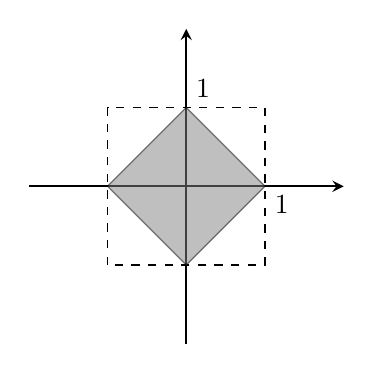
\begin{tikzpicture}
\draw[thick,-stealth] (-2, 0) -- (2, 0);
\draw[thick,-stealth] (0, -2) -- (0, 2);

\draw[dashed] (-1, -1) rectangle (1, 1);
\filldraw[draw=black, fill=gray, opacity=0.5] (-1, 0) -- (0, 1) -- (1, 0) -- (0, -1) -- (-1, 0);
\node [below right] at (1, 0) {1};
\node [above right] at (0, 1) {1};
\end{tikzpicture}
}
	%\caption{$L_{2}$ norm ball}
	\label{}
\end{figure}

(a) First see inside the box, clearly $\vert x_{1}\vert\leq 1$ and $\vert x_{2}\vert\leq 1$

(b) Look at the position we want, $x_{1}+x_{2}\leq 1$, i.e., $x_{2}\leq 1-x_{1}$

(c) Rest by symmetry

\newpage
$L_{\infty}$ norm ball: $\{x|\max\{\vert x_{1}\vert, \vert x_{2}\vert\} \leq 1\}$

\begin{figure}
	\centering
	\resizebox{7.5cm}{3cm}{%% page 15
%% fig 3
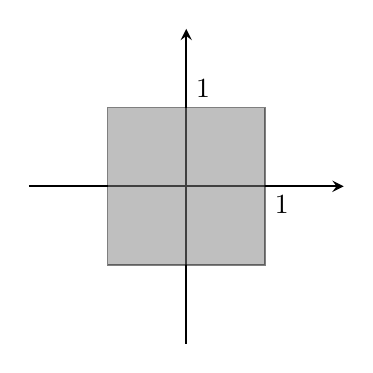
\begin{tikzpicture}
\draw[thick,-stealth] (-2, 0) -- (2, 0);
\draw[thick,-stealth] (0, -2) -- (0, 2);

\filldraw[fill=gray, draw=black, opacity=0.5] (-1, -1) rectangle (1, 1);
\node [below right] at (1, 0) {1};
\node [above right] at (0, 1) {1};
\end{tikzpicture}
}
%	\caption{$L_{\infty}$ norm ball}
	\label{}
\end{figure}

What about card($x$)? 

\begin{figure}
	\centering
	\resizebox{7.5cm}{3cm}{%% page 15
%% fig 4
\begin{tikzpicture}
\draw[thick,-stealth] (-2, 0) -- (2, 0);
\draw[thick,-stealth] (0, -2) -- (0, 2);

\draw (-1, 0) -- (1, 0)node[below]{1};
\draw (0, -1) -- (0, 1)node[right]{1};

\fill (0, 1) circle (1pt);
\fill (1, 0) circle (1pt);
\fill (0, -1) circle (1pt);
\fill (-1, 0) circle (1pt);
\end{tikzpicture}}
%	\caption{}
	\label{}
\end{figure}

The set $\{x|\text{card}(x)\leq 1\}$ obviously is not much of a "ball".

\vspace{0.5cm}
To visualize a bit more, we look at the \textbf{"level sets"} of the norm balls. We define the level set as $\{x|\vert x\vert=c \}$, and let's see for $c=\frac{1}{2}, 1, 2$. See for the figures on the r.h.s.

\begin{marginfigure}
	\centering
	\resizebox{7.5cm}{3cm}{%% page 16
%% fig 1
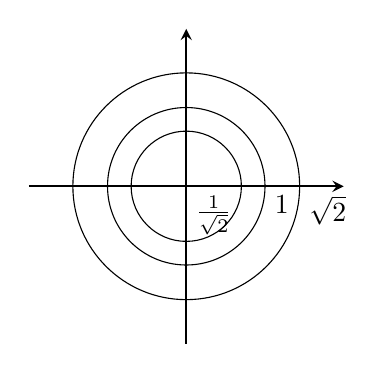
\begin{tikzpicture}
\draw[thick,-stealth] (-2, 0) -- (2, 0);
\draw[thick,-stealth] (0, -2) -- (0, 2);

\draw (0,0) circle [radius=0.7];
\node [below left] at (0.7, 0) {$\frac{1}{\sqrt 2}$};

\draw (0,0) circle [radius=1];
\node [below right] at (1, 0) {1};

\draw (0,0) circle [radius=1.44];
\node [below right] at (1.44, 0) {$\sqrt 2$};

\end{tikzpicture}
}
	\caption{$L_{1}$ level set}
	\label{}
\end{marginfigure}

\begin{marginfigure}
	\centering
	\resizebox{7.5cm}{3cm}{%% page 16
%% fig 2
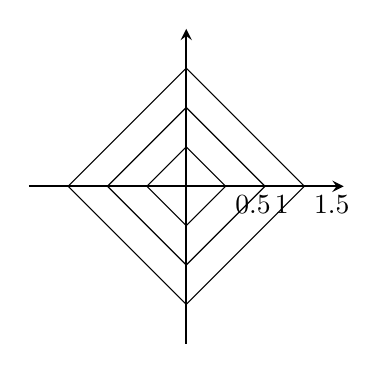
\begin{tikzpicture}
\draw[thick,-stealth] (-2, 0) -- (2, 0);
\draw[thick,-stealth] (0, -2) -- (0, 2);

\draw (-0.5, 0) -- (0, 0.5) -- (0.5, 0) -- (0, -0.5) -- (-0.5, 0);
\node [below right] at (0.5, 0) {0.5};

\draw (-1, 0) -- (0, 1) -- (1, 0) -- (0, -1) -- (-1, 0);
\node [below right] at (1, 0) {1};

\draw (-1.5, 0) -- (0, 1.5) -- (1.5, 0) -- (0, -1.5) -- (-1.5, 0);
\node [below right] at (1.5, 0) {1.5};
\end{tikzpicture}

}
	\caption{$L_{2}$ level set}
	\label{}
\end{marginfigure}

\begin{marginfigure}
	\centering
	\resizebox{7.5cm}{3cm}{%% page 16
%% fig 3
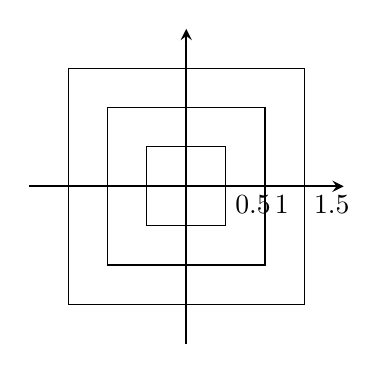
\begin{tikzpicture}
\draw[thick,-stealth] (-2, 0) -- (2, 0);
\draw[thick,-stealth] (0, -2) -- (0, 2);

\draw (-0.5, -0.5) rectangle (0.5, 0.5);
\node [below right] at (0.5, 0) {0.5};

\draw (-1, -1) rectangle (1, 1);
\node [below right] at (1, 0) {1};

\draw (-1.5, -1.5) rectangle (1.5, 1.5);
\node [below right] at (1.5, 0) {1.5};
\end{tikzpicture}
}
	\caption{$L_{\infty}$ level set}
	\label{}
\end{marginfigure}

\vspace{0.3cm}
Why might we be interested in different norms?

Later in the course, we will see applications in optimal control that we want to meet a control objective while minimizing some resources(The objective will be to min a norm of the resources). %For instances,

%$L_2$ $\rightarrow$ get min energy solution.

%$L_1$ $\rightarrow$ get a sparse solution not many forms of jet, useful when "XXX up" overhead

%$L_\infty$ $\rightarrow$ all uses of resource will be equal in magnitude "bang bang "control in vehicles.

\vspace{0.5cm}
\noindent\textbf{Inner Products}

Any inner product(aka dot/scalar product) on a (real) vector space $\Omega$ maps a pair of elements $x, y\in\Omega$ into the scalar, that is, $\langle\cdot,\cdot\rangle:\Omega\times\Omega\mapsto\reals$. For vectors in $\reals^{n}$ the inner product of vectors $x$ and $y$ is given by 
$$\langle x,y\rangle=x^{\trans}y=\sum_{k=1}^{n}x_{k}y_{k}$$


For any $x, y, z\in\Omega$ and $a\in\reals$, the following must hold for a inner product:

(1) $\langle x,y\rangle\geq 0$ and $\langle x,y\rangle=0$ iff $x=0\in\Omega$

(2) $\langle x+y,z\rangle=\langle x,z\rangle+\langle y,z\rangle$

(3) $\langle ax,y\rangle=a\langle x,y\rangle$

(4) $\langle x,y\rangle=\langle y,x\rangle$

\vspace{0.2cm}
Note:

(a) The above change slightly in complex vector space, e.g., $\langle x,y\rangle=\overline{\langle y,x\rangle}$

(b) The concept we develop apply beyond list vectors in $\reals^{n}$ or $\complex_{n}$, e.g., space of polynomials or of functions, but our focus will be $\reals^{n}$ and $\complex_{n}$.


\vspace{0.5cm}
Let's connect to angle now.

\begin{figure}
	\centering
	\resizebox{7.5cm}{3cm}{%% page 18
\begin{tikzpicture}
\coordinate (O) at (0, 0);
\coordinate (A) at (4, 2);
\coordinate (B) at (1, 2);

\draw [ -stealth] (O) -- (A)node[below]{$x$};
\draw [ -stealth] (O) -- (B)node[above]{$y$};

\draw[dashed, -stealth] ($(O)!(B)!(A)$) -- (B)node[above, midway]{$\vec e$};

\draw [ -stealth] (O) -- ($(O)!(B)!(A)$)node[below right]{$x^{'}$};

\draw (A) -- (O) -- (B)
pic [draw= black, angle radius= 0.5cm, "$\theta$"] {angle = A--O--B};
\end{tikzpicture}
}
	\caption{}
	\label{}
\end{figure}

In above picture $x, y\in\reals^{n}$ but since $\text{dim}{\text{span}({x, y})}=2$ (assuming $x$ and $y$ are not co-linear). The familiar picture in $\reals^{2}$ shall holds.

Since we know that $\vert\cos\theta\vert <1$, rearranging gives
$$\vert\langle x,y\rangle\vert =\vert x^{\trans}y\vert \leq \Vert x\Vert_{2} \Vert y\Vert_{2}$$

This is the so called Cauchy-Schwartz inequality, and it relates inner product(angle) to norms(length). Such inequality holds for inner product spaces, not just $\reals^{n}$($n$-dimensional Euclidean space). Further more, it could relate the inner product to the norms (not only $L_{2}$) via a generalization, says, ``H\"older's inequality'':
$$\vert x^{\trans}y\vert\leq \sum_{k=1}^{n}\vert x_{k}y_{k}\vert \leq \Vert x\Vert_{p}\Vert y\Vert_{q}$$

for any $p, q\geq 1$ such that $1/p+1/q=1$.

(1) If $p=q=2$, we get the Cauchy-Schwartz inequality.

(2) If $p=1$, $q=\infty$, we get $\vert x^{\trans}y\vert\leq \Vert x\Vert_{1}\Vert y\Vert_{\infty}=(\sum_{k=1}^{n}\vert x_{k}\vert)(\max_{k\in [n]}x_{k})$.


\vspace{0.5cm}
A second important connection of inner product and norm is that
$$\Vert x\Vert_{2}=\sqrt{x^{\trans} x}=\langle x,x\rangle$$

The $L_{2}$ norm is "induced" by the inner product. In fact, any inner product induces a norm (by the properties of inner product). However, there are norms that are not induced by any inner product, e.g., $L_{1}$ and $L_{\infty}$. Inner product space has a more special structure than a "normed" vector space.

\begin{figure}
	\centering
	\resizebox{7.5cm}{3cm}{% page 19
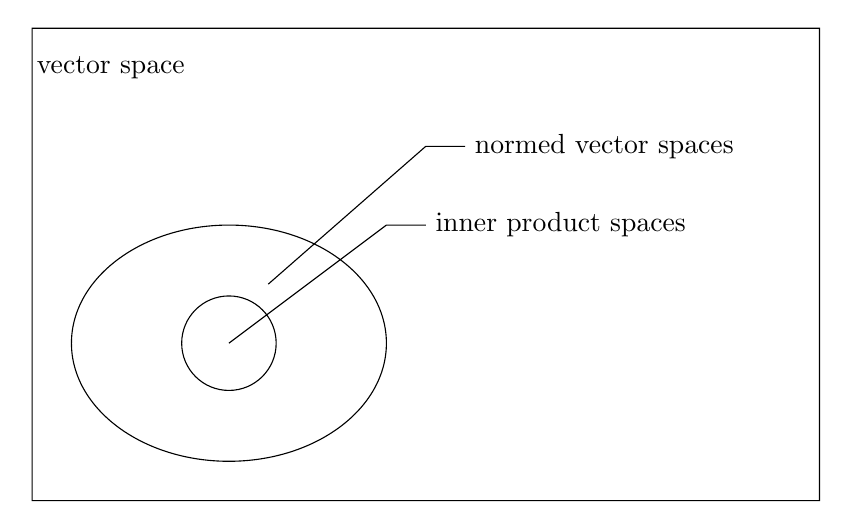
\begin{tikzpicture}
    \path 
        (0, 0) rectangle (10, 6) [draw]
        (1, 5.5) node {vector space}

        (2.5,2) coordinate (A) node[below] { } ellipse (2 and 1.5) [draw]
        
        coordinate (temp) at (2.5, 2) ellipse (0.6 and 0.6) [draw]
        (temp) +(0.5, 0.75) coordinate (B) node[below left] { } -- (5, 4.5) -- (5.5, 4.5) node[right]{normed vector spaces}

        (A) -- (4.5, 3.5) -- (5, 3.5) node[right]{inner product spaces} ;

\end{tikzpicture}
}
	\caption{}
	\label{}
\end{figure}

Note: There are also spaces with a sense of length (a "metric"). Those are not vector spaces (it can't add and scale elements). Those are "metric" spaces.

\vspace{0.5cm}
\noindent\textbf{Angles between vectors}

By Cauchy-Schwartz $\frac{\vert \langle x,y\rangle\vert}{\Vert x\Vert \Vert y\Vert}\leq 1$, hence we have the following cases for the angle $\theta$:

\begin{marginfigure}
	\centering
	\resizebox{7.5cm}{3cm}{%% page 20
%% fig 1
\begin{tikzpicture}
\draw [white, <->] (0, 5) -- (0, 0) -- (5, 0);
\draw [-latex, ultra thick] (0, 0) -- (2, 2);
\node [below] at (3, 2) {$x$};
\node [below] at (2, 2) {$\cos e = 1$};
\draw [-latex, ultra thick] (2, 2) -- (4, 4);
\node [below] at (5, 4) {$y$};
\end{tikzpicture}
}
	\caption{(a) $\cos\theta = +1$}
	\label{}
\end{marginfigure}

\begin{marginfigure}
	\centering
	\resizebox{7.5cm}{3cm}{%% page 20
%% fig 2
\begin{tikzpicture}
\draw [white, <->] (0, 5) -- (0, 0) -- (5, 0);
\draw [-latex, ultra thick] (2, 2) -- (0, 0);
\node [below] at (1, 0) {$y$};
\filldraw[black] (2, 2) circle (2pt) node[anchor=west] {$\cos e = -1$};
\draw [-latex, ultra thick] (2, 2) -- (4, 4);
\node [above] at (5, 4) {$x$};
\end{tikzpicture}

}
	\caption{(a) $\cos\theta = -1$}
	\label{}
\end{marginfigure}

\begin{marginfigure}
	\centering
	\resizebox{7.5cm}{3cm}{%% page 20
%% fig 3
\def\RightAngle[size=#1](#2,#3,#4){%
 \draw ($(#3)!#1!(#2)$) -- 
       ($($(#3)!#1!(#2)$)!#1!90:(#2)$) --
       ($(#3)!#1!(#4)$);
 \path (#3) --
 ($($(#3)!#1!(#2)$)!#1!90:(#2)$);
}
\begin{tikzpicture}
\coordinate (A) at (0, 2);
\coordinate (B) at (5, 2);
\coordinate (C) at (1, 0);

\draw [white, <->] (0, 5) -- (0, 0) -- (5, 0);

\draw [-latex, ultra thick] (C) -- (A);
\node [below] at (0, 3) {$x$};

\draw [-latex, ultra thick] (C) -- (B);
\node [below] at (4, 1) {$y$};

%% right angle
\RightAngle[size=10pt](B,C,A);

\end{tikzpicture}
}
	\caption{(b) $\cos\theta = 0$}
	\label{}
\end{marginfigure}

\begin{marginfigure}
	\centering
	\resizebox{7.5cm}{3cm}{%% page 20
%% fig 4
\begin{tikzpicture}
\draw [<-] (0, 5) -- (0, -1);
\draw [->] (-1, 0) -- (5, 0);

\draw [-latex, ultra thick] (0, 0) -- (5, 0);
\node [below] at (5, 0) {$x$};

\draw [-latex, ultra thick] (0, 0) -- (3, 3);
\node [below right] at (3, 3) {$y$};

\draw (1, 0) coordinate (A) -- (0, 0) coordinate (B) -- (1, 1) coordinate (C)
pic [draw= black, angle radius= 1cm] {angle};
\node [below right] at (1, 0.5) {$o$};
\end{tikzpicture}
}
	\caption{(c) $\cos\theta>0$}
	\label{}
\end{marginfigure}

\begin{marginfigure}
	\centering
	\resizebox{7.5cm}{3cm}{%% page 20
%% fig 5
\begin{tikzpicture}
\draw [<-] (0, 5) -- (0, -1);
\draw [->] (-5, 0) -- (5, 0);

\draw [-latex, ultra thick] (0, 0) -- (5, 0);
\node [below] at (5, 0) {$x$};

\draw [-latex, ultra thick] (0, 0) -- (-3, 3);
\node [below right] at (-3, 3) {$y$};

\draw (1, 0) coordinate (A) -- (0, 0) coordinate (B) -- (-1, 1) coordinate (C)
pic [draw= black, angle radius= 1cm] {angle};
\node [below right] at (1, 1) {$o$};
\end{tikzpicture}}
	\caption{(c) $\cos\theta<0$}
	\label{}
\end{marginfigure}

(a) If $\vert\cos\theta\vert = +1$, then $\theta=0^{\circ}$ or $180^{\circ}$. Vectors $x$ and $y$ are "co-linear", and $\vert\langle x,y\rangle\vert=\Vert x\Vert \Vert y\Vert$


(b) If $\vert\cos\theta\vert = 0$, then $\theta = 90^{\circ}$, and $\frac{\vert\langle x,y\rangle\vert}{\Vert x\Vert \Vert y\Vert}=0$, or equivalently, $\langle x,y\rangle=0$ (assuming $x\neq 0$ and $y\neq 0$). In this case, $\theta$ is a "right" angle, and $x$, $y$ are orthogonal vectors.

(c) If $\vert \theta\vert <90^{\circ}$ ,then $\cos\theta >0$, and $\langle x,y\rangle >0$, and $\theta$ is a "acute angle", whereas if $\vert \theta\vert >90^{\circ}$, then $\cos\theta <0$ and $\langle x,y\rangle <0$, $\theta$ is a "obtuse angle".



\vspace{0.5cm}
\noindent\textbf{Orthogonality}

A set of vectors $S=\{x^{(1)}, x^{(2)},\cdots, x^{(m)}\}$ is mutually orthogonal if $\langle x^{(i)},x^{(j)}\rangle =0$, $\forall i\neq j$
					
Such sets have nice property that the elements of S are linearly independent and so provide a basis for span($S$) and hence dim(span($S$))=$m$.

If, in addition, all elements have unit norm, i.e., $\Vert x^{(i)}\Vert_{2}=1$ for all $i\in[m]$ then the set forms an \textbf{orthogonal basis}.

Note that we use $\Vert\cdot\Vert_{2}$ to measure length because it is induced by the inner product.


%\begin{marginfigure}
%	\centering
%	\resizebox{7.5cm}{3cm}{%% page 21
%% fig 1
\def\RightAngle[size=#1](#2,#3,#4){%
 \draw ($(#3)!#1!(#2)$) -- 
       ($($(#3)!#1!(#2)$)!#1!90:(#2)$) --
       ($(#3)!#1!(#4)$);
 \path (#3) --
 ($($(#3)!#1!(#2)$)!#1!90:(#2)$);
}
\begin{tikzpicture}
\node [below right] at (2, -1) {orthogonal};
\draw [<-] (0, 5) -- (0, -3);
\draw [->] (-3, 0) -- (5, 0);

\coordinate (A) at (5, -5);
\coordinate (B) at (-3, -3);
\coordinate (O) at (0, 0);

\draw [-latex, ultra thick] (O) -- (A);
\node [below] at (5, -5) {$x^{1}$};

\draw [-latex, ultra thick] (O) -- (B);
\node [below right] at (-3, -3) {$x^{2}$};

%% right angle
\RightAngle[size=10pt](B,O,A);

\end{tikzpicture}
}
%	\caption{}
%	\label{}
%\end{marginfigure}

%\begin{marginfigure}
%	\centering
%	\resizebox{7.5cm}{3cm}{%% page 21
%% fig 2
\def\RightAngle[size=#1](#2,#3,#4){%
 \draw ($(#3)!#1!(#2)$) -- 
       ($($(#3)!#1!(#2)$)!#1!90:(#2)$) --
       ($(#3)!#1!(#4)$);
 \path (#3) --
 ($($(#3)!#1!(#2)$)!#1!90:(#2)$);
}
\begin{tikzpicture}
\node [below right] at (2, -1) {orthogonal};
\draw [<-] (0, 5) -- (0, -3);
\draw [->] (-3, 0) -- (5, 0);

\coordinate (A) at (3, -3);
\coordinate (B) at (-3, -3);
\coordinate (O) at (0, 0);

\draw [-latex, ultra thick] (O) -- (A);
\node [below] at (5, -5) {$x^{1}$};

\draw [-latex, ultra thick] (O) -- (B);
\node [below right] at (-3, -3) {$x^{2}$};

%% right angle
\RightAngle[size=10pt](B,O,A);

\end{tikzpicture}}
%	\caption{}
%	\label{}
%\end{marginfigure}

\vspace{0.3cm}
\textbf{Orthogonal complement}: Given a subspace $S\in \nu$, a vector $x\in\nu$ is orthogonal to $S$ if $x\perp s, \forall s\in S$, i.e., $\perp$ to all vectors in the subspace $S$. The orthogonal complement to $S$ is defined as a collection of such vectors $x$, namely
$$ S^{\perp} =\{x\in\nu|x\perp s\}$$

Some results of $S^{\perp}$:

(i) $S^{\perp}$ is a subspace: clearly it includes $0\in\gamma$ and is closed under linear combination(all linear combination $\perp S$).

(ii) dim($\nu$)=dim($S$) + dim ($S^{\perp}$).

(iii) Any $x\in\nu$ can be written in a unique way as $x=x_{s}+x_{s^{\perp}}$ for any subspace $S$.

Note: If $S=\nu$ then $S^{\perp}={0}$.


\vspace{0.5cm}
\noindent\textbf{Projection}

Motivation: Given a point $x\in\nu$, find the "closest" point in the set $S$ (recall that points $\equiv$ vectors), this point is called the projection of $x$ on the set $S$. Denote this point as $y$, formally we have
$$y=\Pi_{s}(x)=\arg \min_{y\in S} \Vert y-x\Vert$$

\vspace{0.3cm}
Let's consider different cases for this optimization question:

(1) $S$ is a subspace of an inner product space associate with $L_{2}$ norm

\begin{marginfigure}
	\centering
	\resizebox{7.5cm}{3cm}{%% page 23
%% fig 1
\begin{tikzpicture}[dot/.style={circle,inner sep=1pt,fill,label={#1},name=#1},
  extended line/.style={shorten >=-#1,shorten <=-#1},
  extended line/.default=1cm]
 \draw[thick,-stealth] (-2.5, 0) -- (4.5, 0);
 \draw[thick,-stealth] (0, -2.5) -- (0, 4.5);

 \coordinate (A) at (-1, -0.75);
 \coordinate (B) at (4, 3);
 \draw [extended line=0cm, -] (A) -- (B) node[pos=1.15, font=\small]{$\mathcal{S}$};     
 \draw [ -stealth] (0,0) -- (1.3, 2.15) coordinate (yn) node[right]{$x$};
 \draw[dashed] (yn) -- ($(A)!(yn)!(B)$);
 \draw [ -stealth] (0,0) -- ($(A)!(yn)!(B)$);
\end{tikzpicture}
}
	\caption{$S$ is a subspace of an inner product space}
	\label{}
\end{marginfigure}

(2) $S$ is an "affine" set(a shifted subspace)

\begin{marginfigure}
	\centering
	\resizebox{7.5cm}{3cm}{%% page 23
%% fig 2
\begin{tikzpicture}[dot/.style={circle,inner sep=1pt,fill,label={#1},name=#1},
  extended line/.style={shorten >=-#1,shorten <=-#1},
  extended line/.default=1cm]
 \draw[thick,-stealth] (-2.5, 0) -- (4.5, 0);
 \draw[thick,-stealth] (0, -2.5) -- (0, 4.5);

 \coordinate (A) at (-1, 0.25);
 \coordinate (B) at (4, 4);
 \draw [extended line=0cm, -] (A) -- (B) node[pos=1.15, font=\small]{$\mathcal{A}$};     
 \draw [ -stealth] (0,0) -- (1, 3) coordinate (yn) node[right]{$x$};
 \draw[dashed] (yn) -- ($(A)!(yn)!(B)$);
\end{tikzpicture}}
	\caption{$S$ is an "affine" set}
	\label{}
\end{marginfigure}

(3) Consider other norms, e.g., $L_{1}$, $L_{\infty}$ for which no inner product(projection in normed vectors space)

\vspace{0.3cm}
\textbf{Projection onto 1-D subspace}

Let's consider the one dimension subspace given by
$$S=span(\{v\})=\{\lambda v|\lambda \in \reals\}$$

The vector $x$ and subspace $S$ are something like:
\begin{figure}
	\centering
	\resizebox{7.5cm}{3cm}{%% page 24
\def\RightAngle[size=#1](#2,#3,#4){%
 \draw ($(#3)!#1!(#2)$) -- 
       ($($(#3)!#1!(#2)$)!#1!90:(#2)$) --
       ($(#3)!#1!(#4)$);
 \path (#3) --
 ($($(#3)!#1!(#2)$)!#1!90:(#2)$);
}
\begin{tikzpicture}
 \coordinate (A) at (-1, -0.75);
 \coordinate (B) at (4, 3);
 \coordinate (O) at (0, 0);

 \draw (A) -- (B) node[pos=1.15, font=\small]{$\mathcal{S}$};
 \filldraw[black] (O) circle (1pt) node[anchor=west] {$O$};
 \draw [ -stealth] (A) -- (3, 2.25) coordinate (yn) node[right]{$v$};
 \draw [ -stealth] (O) -- (1, 2.7) coordinate (yn) node[right]{$x$};
 \draw[dashed] (yn) -- ($(A)!(yn)!(B)$);
 \draw [ -stealth] (0,0) -- ($(A)!(yn)!(B)$) node[right]{$x_S$};
 
 \coordinate (S) at ($(A)!(yn)!(B)$);
 %% right angle
 \RightAngle[size=10pt](B,S,yn);

\end{tikzpicture}}
	\caption{}
	\label{}
\end{figure}

By orthogonal decomposition,  $x\in S\oplus S^{\perp}$, and therefore $\exists x_{s}\in S, e\in S^{\perp}$, such that $x=x_{s}+e$ (an unique expression).

Use this decomposition to solve the optimization problem(find the closest point)
$$\Pi_{s}(x)=\arg_{y\in S} \min \Vert y-x\Vert_{2}=\arg_{y\in S} \min \Vert y-x\Vert_{2}^{2}$$

The objective function can be written as
\begin{align*}
\Vert y-x\Vert_{2}^{2}&=\langle y-x,y-x\rangle\\
&=\langle (y-x_{s})-e,(y-x_{s})-e\rangle\\
&=\Vert y-x_{s}\Vert^{2} + \Vert z\Vert^{2} - 2\langle y-x_{s},e\rangle\\
&\geq \Vert e\Vert_{2}^{2}
\end{align*}

where the minimum is attained by setting $y=x_{s}$. Note that the minimum is unique by uniqueness of orthogonal decomposition and $\Vert y-x_{s}\Vert^{2}=0$ iff $y=x_{s}$.

To summarize, 
$$x_{s}=\Pi_{s}(x)=\arg_{y\in S} \min \Vert y-x\Vert_{2}$$

where $x_{s}$ is in $\perp$-decomposition.

To solve for $x_{s}$ (the point we want), we use the condition that
$$(x-x_{s}) \perp S=\{\lambda v|\lambda\in\reals\}$$

Since $x\in S$, $\exists a\in\reals$ such that $x_{s}=av$, and now we need to solve for $a$ by
$$0=\langle x-av,v\rangle=\langle x,v\rangle-\langle av,v\rangle=\langle x,v\rangle-a\langle v,v\rangle$$

Rearranging yields that $a=\frac{\langle x,v\rangle}{a\langle v,v\rangle}=\frac{\langle x,v\rangle}{\Vert v\Vert^{2}}$. Thus, $x_{s}=av=\frac{\langle x,v\rangle}{\Vert v\Vert^{2}}v$.


\vspace{0.5cm}
\textbf{Projection onto a general subspace}

Observe that all previous steps for 1-D case still hold. Only used $S$ is 1-D when solving for $x^{(s)}$, so we have already done.

\textbf{Theorem}: Let $x\in\Omega$ and $S\in\Omega$, where $x$ is a vector, $S$ is a subspace of $\Omega$ and $\Omega$ is an inner product space. There exists a unique vector $x^{*}\in S$ such that
$$x^{*} = \arg_{y\in S}\min \Vert x-y\Vert$$

A necessary and sufficient condition for $x^{*}$ is

(1). $x^{*} \in S$

(2). $x-x^{*}\perp S$

\vspace{0.3cm}
Now let's consider how to solve for $x^{*}$ in this general case.

Let $S=\text{span}\left(\{x^{(1)},x^{(2)},\cdots\,x^{(d)}\}\right)$. Notice that $x^{*}\in S$ can be written as $x^{*}=\sum_{i=1}^{d}a_{i}x^{(i)}$ for some $a_{i}$, and $(x-x^{*}) \perp S$, then if $(x-x^{*}) \perp x^{(k)}$ $\forall k\in [d]$, that will be $\perp$ to all linear combination of the spanning set and hence $\perp$ to $S$.

Accordingly yields $d$ conditions, $\forall k\in [d]$, we have
$$0=\langle x-x^{*},x^{(k)}\rangle=\langle x-\sum_{i=1}^{d}a_{i}x^{(i)},x^{(k)}\rangle=\langle x,x^{(k)}\rangle-\sum_{i=1}^{d}a_{i}\langle x^{(i)},x^{(k)}\rangle$$

Rearranging yields
$$\sum_{i=1}^{d}a_{i}\langle x^{(i)},x^{(k)}\rangle=\langle x,x^{(k)}\rangle ,\ \forall k\in [d]$$

Or stacking into a matrix($d$ equations in $d$ unknowns)
$$\left[ 
\begin{array}{cccc} 
\langle x^{(1)},x^{(1)}\rangle & \langle x^{(1)},x^{(2)}\rangle &\cdots& \langle x^{(1)},x^{(d)}\rangle\\
\vdots&&& \\
\langle x^{(d)},x^{(1)}\rangle & \cdots &\cdots& \langle x^{(d)},x^{(d)}\rangle
\end{array}
\right]
\left[ 
\begin{array}{c} 
d_{1}\\
\vdots\\
d_{d}
\end{array}
\right]=
\left[ 
\begin{array}{c} 
\langle x^{(1)},x\rangle\\
\vdots\\
\langle x^{(a)},x\rangle\\
\end{array}
\right]$$

One case where easy to solve the equation is, when the $x^{(k)}$ are all mutually $\perp$ (so the matrix is diagonal), or furthermore, all these vectors have unit length and mutually orthogonal(so it is an identity matrix).

\vspace{0.3cm}
How do you orthogonalize and normalize a matrix?

\textbf{Gram-Schmidt Procedure:}

Let's consider an example: we have already have a basis ${x^{(1)}, x^{(2)}}$, and we want to find the orthogonal basis ${z^{(1)}, z^{(2)}}$.

\begin{marginfigure}
	\centering
	\resizebox{7.5cm}{3cm}{%% page 28
%% fig 1
\begin{tikzpicture}
\coordinate (O) at (0, 0);
\coordinate (A) at (3, 0);
\coordinate (B) at (2, 2);

\draw [ -stealth] (O) -- (A) node[pos=1.15, font=\small]{$x^{(1)}$};
\draw [ -stealth] (O) -- (B) node[pos=1.15, font=\small]{$x^{(2)}$};
\end{tikzpicture}
}
	\caption{Problem setting}
	\label{}
\end{marginfigure}

\begin{marginfigure}
	\centering
	\resizebox{7.5cm}{3cm}{%% page 28
%% fig 2
\def\RightAngle[size=#1](#2,#3,#4){%
 \draw ($(#3)!#1!(#2)$) -- 
       ($($(#3)!#1!(#2)$)!#1!90:(#2)$) --
       ($(#3)!#1!(#4)$);
 \path (#3) --
 ($($(#3)!#1!(#2)$)!#1!90:(#2)$);
}
\begin{tikzpicture}
\coordinate (O) at (0, 0);
\coordinate (A) at (3, 0);
\coordinate (B) at (2, 2);

\draw [ -stealth] (O) -- (A) node[pos=1.15, font=\small]{$x^{(1)}$};
\draw [ -stealth] (O) -- (B) node[pos=1.15, font=\small]{$x^{(2)}$};

\coordinate (C) at ($(O)!(B)!(A)$);
\draw[dashed] (B) -- (C);

%% right angle
\RightAngle[size=10pt](A,C,B);

\draw [ -stealth] (O) -- (C) node[below]{$u$};
\draw [ -stealth] (O) -- (1, 0) node[below]{$z^{(1)}$};

\end{tikzpicture}
}
	\caption{Step 1}
	\label{}
\end{marginfigure}

\begin{marginfigure}
	\centering
	\resizebox{7.5cm}{3cm}{%% page 28
%% fig 3
\begin{tikzpicture}
\coordinate (O) at (0, 0);
\coordinate (A) at (3, 0);
\coordinate (B) at (2, 2);
\coordinate (C) at (0, 3);

\draw [ -stealth] (O) -- (A) node[pos=1.15, font=\small]{$x^{(1)}$};
\draw [ -stealth] (O) -- (B) node[pos=1.15, font=\small]{$x^{(2)}$};

\draw[dashed] (B) -- ($(O)!(B)!(A)$);

\draw [ -stealth] (O) -- ($(O)!(B)!(A)$) node[below]{$u$};
\draw [ -stealth] (O) -- (1, 0) node[below]{$z^{(1)}$};

\draw (O) -- (C);
\draw[dashed] (B) -- ($(O)!(B)!(C)$);

\draw [ -stealth] (O) -- ($(O)!(B)!(C)$) node[left]{$x^{(2)}-u$};
\draw [ -stealth] (O) -- (0, 1) node[left]{$z^{(2)}$};
\end{tikzpicture}}
	\caption{Step 2}
	\label{}
\end{marginfigure}

Step 1: Normalize $x^{(1)}$
$$z^{(1)}=\frac{x^{(1)}}{\Vert x^{(1)}\Vert}$$

Step 2: Orthogonalize $x^{(2)}$

\quad (a). Project $x^{(2)}$ onto $z^{(1)}$
$$\frac{\langle x^{(2)},z^{(1)}\rangle}{\Vert z^{(1)}\Vert} z^{(1)}=\langle x^{(2)},x^{(1)}\rangle z^{(1)}=u$$

\quad (b). Normalize to obtain $z^{(2)}$
$$\frac{x^{(2)}-u}{\Vert x^{(2)}-u\Vert}$$

The above procedure could be extended to higher dimensions as needed.

\vspace{0.4cm}
Stacking up results and yields the \textbf{QR decomposition}
\begin{align*}
	A&=\left[\begin{matrix}
	\vdots&\vdots&\cdots&\vdots\\
	x^{(1)}&x^{(2)}&\cdots&x^{(m)}\\
	\vdots&\vdots&\cdots&\vdots
	\end{matrix}\right]=\left[\begin{matrix}
	\vdots&\vdots&\cdots&\vdots\\
	z^{(1)}&z^{(2)}&\cdots&z^{(m)}\\
	\vdots&\vdots&\cdots&\vdots
	\end{matrix}\right]
	\left[\begin{matrix}
	r_{11}&r_{12}&r_{13}&\cdots\\
	0&r_{22}&r_{23}&\cdots\\
	0&0&r_{33}&\cdots\\
	\vdots&\ddots& & 
	\end{matrix}\right]\\
	&=QR\\
	&=\left[\begin{matrix}
	\vdots&\vdots&\cdots\\
	r_{11}z^{(1)}&r_{12}z^{(1)}+r_{22}z^{(1)}&\cdots \\
	\vdots&\vdots&\cdots 
	\end{matrix}\right]
\end{align*}

Note that any non singular square matrix $A$ could be decomposed in this way.

\vspace{0.5cm}
\textbf{Project onto affine set}

Recall that all subspace must go through origin, and an "affine" set is a shift/translate of a subspace, and thus it seems that it can't be too difficult to project onto this kind of set. An affine set $\mathcal{A}$ is defined as

\begin{marginfigure}
	\centering
	\resizebox{7.5cm}{3cm}{%% page 30
%% fig 1
\def\RightAngle[size=#1](#2,#3,#4){%
 \draw ($(#3)!#1!(#2)$) -- 
       ($($(#3)!#1!(#2)$)!#1!90:(#2)$) --
       ($(#3)!#1!(#4)$);
 \path (#3) --
 ($($(#3)!#1!(#2)$)!#1!90:(#2)$);
}
\begin{tikzpicture}[dot/.style={circle,inner sep=1pt,fill,label={#1},name=#1},
  extended line/.style={shorten >=-#1,shorten <=-#1},
  extended line/.default=1cm]
\draw[thick,-stealth] (-2.5, 0) -- (4.5, 0);
\draw[thick,-stealth] (0, -2.5) -- (0, 4.5);

\coordinate (O) at (0, 0) node[below right]{$O$};
\coordinate (A) at (4, 2);
\coordinate (B) at (3, 4);
\coordinate (D) at ($(O)!(B)!(A)$);

\draw [extended line=1.75cm, -] (O) -- (A) node[pos=1.5, font=\small]{$\mathcal{S}$};
\draw [ -stealth] (O) -- (B) node[right]{$x$};
\draw[dashed] (B) -- (D);
\draw [ -stealth] (O) -- (D) node[below]{$x_S$};

%% right angle
\RightAngle[size=10pt](B,D,O);

\end{tikzpicture}

}
	\caption{Subpace $S$}
	\label{}
\end{marginfigure}

\begin{marginfigure}
	\centering
	\resizebox{7.5cm}{3cm}{%% page 30
%% fig 2
\def\RightAngle[size=#1](#2,#3,#4){%
 \draw ($(#3)!#1!(#2)$) -- 
       ($($(#3)!#1!(#2)$)!#1!90:(#2)$) --
       ($(#3)!#1!(#4)$);
 \path (#3) --
 ($($(#3)!#1!(#2)$)!#1!90:(#2)$);
}
\begin{tikzpicture}[dot/.style={circle,inner sep=1pt,fill,label={#1},name=#1},
  extended line/.style={shorten >=-#1,shorten <=-#1},
  extended line/.default=1cm]
\draw[thick,-stealth] (-2.5, 0) -- (4.5, 0);
\draw[thick,-stealth] (0, -2.5) -- (0, 4.5);

\coordinate (O) at (0, 0) node[below right]{$O$};
\coordinate (A) at (4, 3);
\coordinate (B) at (3, 4);
\coordinate (C) at (0, 1);
\coordinate (D) at ($(C)!(B)!(A)$);

\draw [extended line=3cm, -] (C) -- (A) node[below, pos=1.5, font=\small]{$\mathcal{A}$};
\draw [ -stealth] (O) -- (B);
\draw[dashed] (B) -- (D);

%% right angleS
\RightAngle[size=10pt](B,D,C);

\end{tikzpicture}}
	\caption{Affine set $\mathcal{A}$ as a shifted subspace}
	\label{}
\end{marginfigure}

$$\mathcal{A}=\{x\in\Omega|x=u+x^{(0)}, u\in U, x^{(0)}\in \mathcal{A}\}$$

Note that we can shift $S$ be any point in $\mathcal{A}$.

\vspace{0.3cm}
The idea of finding projection onto affine set:

Step (0) Goal: to project $x\in \Omega$ onto $\mathcal{A}$.

Step (1) Translate both $x$ and $\mathcal{A}$ by $-x^{(0)}$, and note that the translation of $\mathcal{A}$ is $S$.

Step (2) Project(translate) $x-x^{(0)}$ onto $S$(as we did before), and shift result back by $+x^{(0)}$.

Step (3) Get the projection point in $\mathcal{A}$.

\begin{marginfigure}
	\centering
	\resizebox{7.5cm}{3cm}{%% page 32
%% fig 1
\begin{tikzpicture}
\draw[thick,-stealth] (-3, 0) -- (3, 0);
\draw[thick,-stealth] (0, -2) -- (0, 4);

\draw (-4, -0.5) -- (3, 3) node[right]{$\mathcal{A}$};    
\draw [dashed, -stealth] (0, 0) -- (1.6, 2.3)node[above]{$x^{(0)}$};
\draw [dashed, -stealth] (0, 0) -- (0.8, 3.4)node[above]{$x$};
\end{tikzpicture}
}
	\caption{Step (0)}
	\label{}
\end{marginfigure}

\begin{marginfigure}
	\centering
	\resizebox{7.5cm}{3cm}{%% page 32
%% fig 2
\begin{tikzpicture}
\draw[thick,-stealth] (-3, 0) -- (3, 0);
\draw[thick,-stealth] (0, -2) -- (0, 4);

\draw (-3, -1.5) -- (3, 1.5) node[right]{$S=\mathcal{A}-x^{(0)}$};
\draw [dashed, -stealth] (-0.8, 1.1)node[left]{$x-x^{(0)}$} -- (0.8, 3.4)node[above]{$x$};
\end{tikzpicture}

}
	\caption{Step (1)}
	\label{}
\end{marginfigure}

\begin{marginfigure}
	\centering
	\resizebox{7.5cm}{3cm}{%% page 32
%% fig 3
\def\RightAngle[size=#1](#2,#3,#4){%
 \draw ($(#3)!#1!(#2)$) -- 
       ($($(#3)!#1!(#2)$)!#1!90:(#2)$) --
       ($(#3)!#1!(#4)$);
 \path (#3) --
 ($($(#3)!#1!(#2)$)!#1!90:(#2)$);
}
\begin{tikzpicture}
\draw[thick,-stealth] (-3, 0) -- (3, 0);
\draw[thick,-stealth] (0, -2) -- (0, 4);

\coordinate (A) at (-3, -1.5);
\coordinate (B) at (3, 1.5);
\coordinate (C) at (-0.8, 1.1);
\coordinate (D) at ($(A)!(C)!(B)$);

\draw (A) -- (B) node[right]{$\mathcal{S}$};
\draw [dashed] (C)node[left]{$x-x^{(0)}$} -- (D)node[below]{$x_{\mathcal{S}}$};

%% right angle
\RightAngle[size=10pt](B,D,C);

\end{tikzpicture}
}
	\caption{Step (2)}
	\label{}
\end{marginfigure}

\begin{marginfigure}
	\centering
	\resizebox{7.5cm}{3cm}{%% page 32
%% fig 4
\def\RightAngle[size=#1](#2,#3,#4){%
 \draw ($(#3)!#1!(#2)$) -- 
       ($($(#3)!#1!(#2)$)!#1!90:(#2)$) --
       ($(#3)!#1!(#4)$);
 \path (#3) --
 ($($(#3)!#1!(#2)$)!#1!90:(#2)$);
}
\begin{tikzpicture}
\draw[thick,-stealth] (-3, 0) -- (3, 0);
\draw[thick,-stealth] (0, -2) -- (0, 4);

\coordinate (A) at (-3, -1.5);
\coordinate (B) at (3, 1.5);
\coordinate (C) at (-0.8, 1.1);
\draw (A) -- (B) node[right]{$\mathcal{S}$};

\coordinate (A1) at (-4, -0.5);
\coordinate (B1) at (3, 3);
\coordinate (C1) at (0.8, 3.4);
\draw (A1) -- (B1) node[right]{$\mathcal{A}$};

\coordinate (D1) at ($(A1)!(C1)!(B1)$);
\draw[dashed] (C1)node[above]{$x$} -- (D1)node[below right]{$x^{*} = x_{\mathcal{S}} + x^{(0)}$};
\draw [dashed, -stealth] ($(A)!(C)!(B)$)node[below]{$x_{\mathcal{S}}$} -- (D1);

%% right angle
\RightAngle[size=10pt](B1,D1,C1);

\end{tikzpicture}}
	\caption{Step (3)}
	\label{}
\end{marginfigure}

\vspace{0.3cm}
\textbf{Theorem: Projection onto affine set}

Let $\mathcal{A}\in \Omega$ be an affine set, where $\Omega$ is an inner product space and $\mathcal{A}=S+x^{(c)}$. There is a unique $x^{*}\in \mathcal{A}$ such that 
$$x^{*} = \arg_{y\in \mathcal{A}}\min \Vert y-x\Vert$$

A necessary and sufficient(set of) conditions:

(1). $x^{*} \in \mathcal{A}$

(2). $(x-x^{*})\perp S$

\vspace{0.3cm}
Proof: Any $y\in A$ can be expressed as $y=z+x^{(0)}$ when $z\in S$
\begin{align*}
\min_{y\in A} \Vert y-x\Vert&=\min_{(z+x^{(0)})\in A} \Vert z+x^{(0)}-x\Vert\\
&=\min_{z\in S} \Vert z-(x-x^{(0)})\Vert
\end{align*}

Thus $z^{*}=\arg\min_{z\in S} \Vert z-(x-x^{(0)})\Vert$, and translating back, we have
$$x^{(*)}=z^{(*)}+x^{(0)}$$


What are the conditions for optimality? That is,

$z^{(*)}-(x-x^{(0)})\perp S$ , where $z^{*}\in S$ is obtained by projection onto $S$.

Thus, in terms of optimal $x^{*}$,

(1) $x^{(*)}=z^{(*)}+x^{(0)} \in A$.

(2) $(z^{(*)}+x^{(0)}-x) \perp S \Leftrightarrow (x^{(*)}-x)\perp S$.


\vspace{0.3cm}
Example: Projection onto a hyperplane

A \textbf{hyperplane} is an affine set $\mathcal{H}$ specified by the pair $(a, b) \in \mathbb{R}^n \times \mathbb{R}$. 
\[
\mathcal{H} = \{ z \in \mathbb{R}^n | a^{T} z = b \}
\] 
An equivalent definition is 
\[
\mathcal{H} = \{ z \in \mathbb{R}^n | z = u + z^{(0)}, u \in S, z^{(0)} \in \mathcal{H} \}
\] 
where $S$ is the subspace $S = \{ z \in \mathbb{R}^n | a^{T} z = 0 \}$. 

Note: 

(1) The "equivalent" definition is clearly that of an affine set.

(2) $a \neq 0$ is termed as the "normal" direction.

(3) If $b \neq 0$, then $\mathcal{H} = \mathcal{S}$ and so it is a subspace. 


\begin{figure}
	\centering
	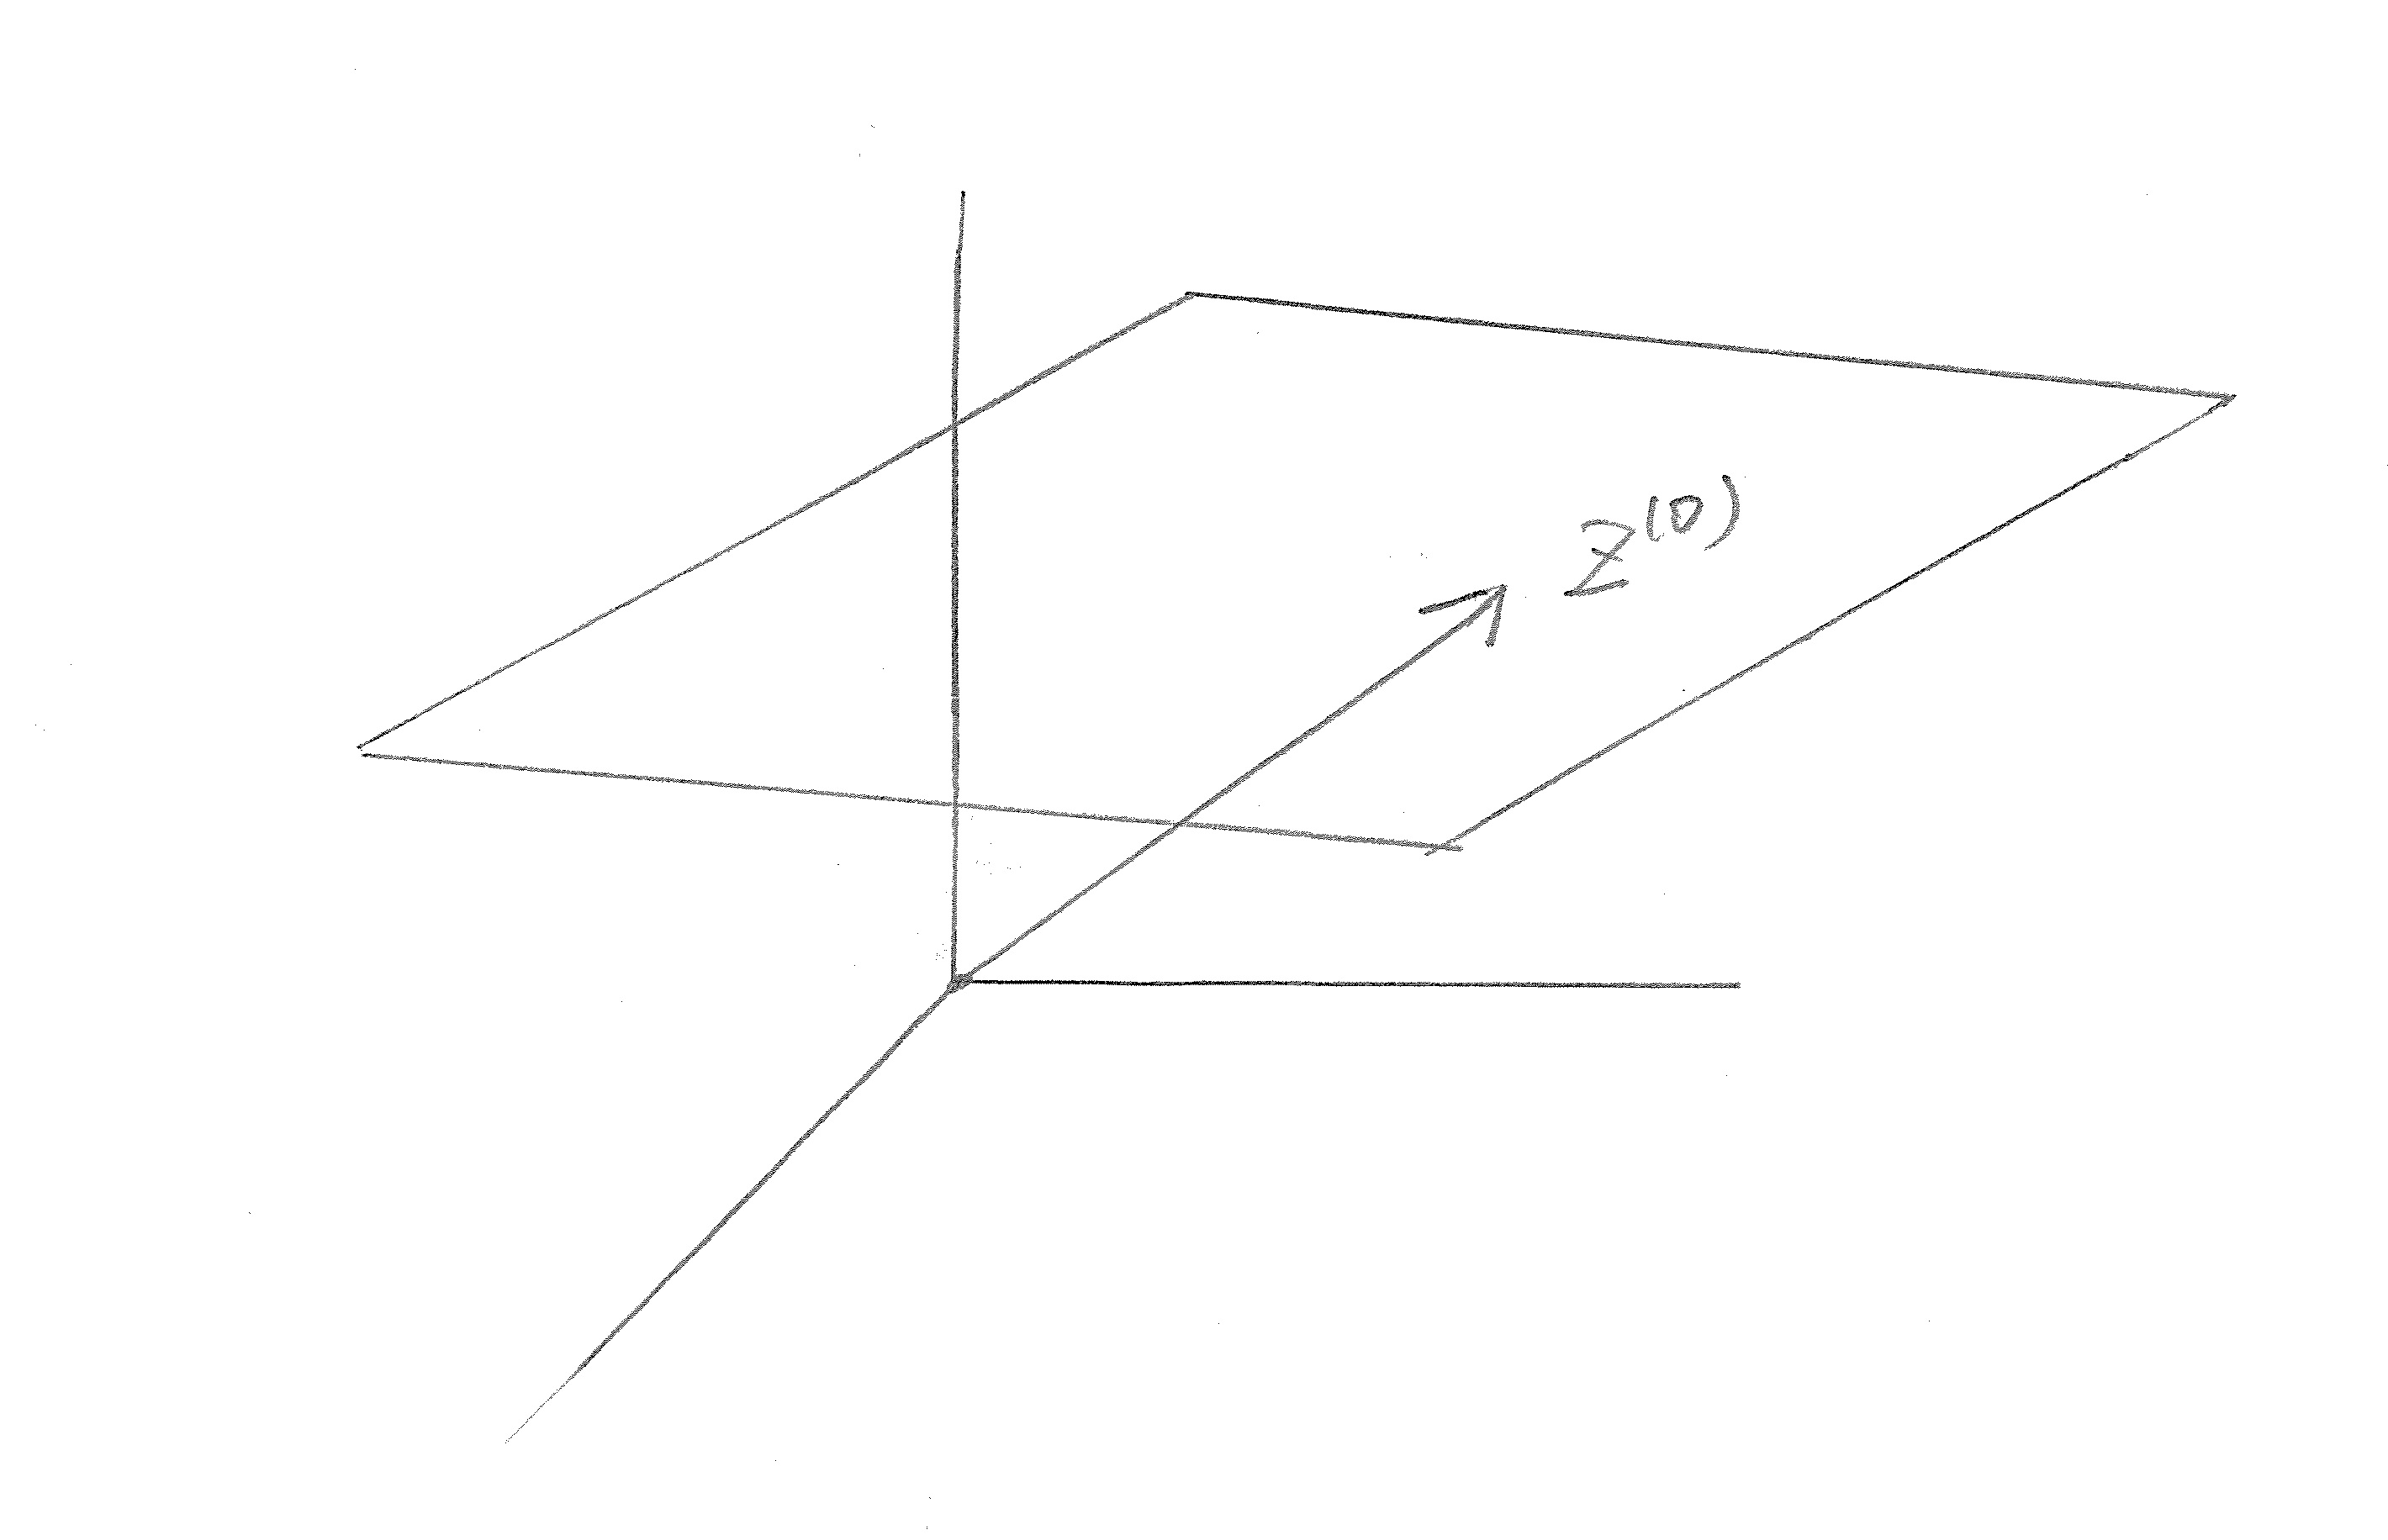
\includegraphics[width=2.1in,height=2.1in]{figures/ch02/p35.jpg}
	%\caption{This is an inserted JPG graphic} 
	%\label{fig:graph} 
\end{figure}

A hyperplane is a special type of affine set. The dimension of the hyperplane is $n-1$ given that the subspace $S$ has a dimension of $n$. For example,

(1) A (2-D) plane is a hyperplane in $\mathbb{R}^3$. 

(2) A line is a hyperplane in $\mathbb{R}^3$. 

(3) A line is not hyperplane in $\reals_{3}$.


\vspace{0.3cm}
Exercise: Prove equivalence of above 2 definition

Let's Start with $\mathcal{H} = \{z \in \mathbb{R}^2 | a^{T} z = b \}$, and let $z^{0} \in \mathcal{H}$(any element at $\mathcal{H}$ will do).

Then, since $a^{T} z^{0} = b$ and for any $z \in \mathcal{H}$, we have

$$a^{T} z - b = 0\Leftrightarrow a^{T} - a^{T}z^{(0)} = 0\Leftrightarrow a^{T} (z - z^{(0)}) = 0$$

Thus,
$$\mathcal{H} = \{z | a^{T} (z - z^{(0)}) = 0 \}     \qquad (*)$$

Now, since $(\text{span} \{ a \}) = \{ x | x= \lambda  a, \lambda \in \mathcal{R} \}$ is a subspace of dim $1$, the set $(\text{span} \{ a \})^{\perp} $ is a subspace of dim $n-1$. 

Let $\mathcal{S}$ be this subspace.

Observe that by (*), vectors in $\mathcal{H}$ when translate by $-z^{(0)}$ on $\mathcal{S}$. 

Therefore $\mathcal{H}$ is $\mathcal{S}$ translated by $+z^{(0)}$ yields $z^{(0)}$. 

Now, let's start with $\mathcal{H} = \{ z \in \mathbb{R}^n | z = u + z^{(0)}, u \in \mathcal{S}, z \in \mathcal{H} \}$. 

Let $\{ u^{(1)}, \dots, u^{(n-1)} \}$ be a basis for $u$, and we choose $a \perp u^{(i)}$, $i \in [n-1]$ and let $b = a^{T} z^{0}$. Then for any $z \in \mathcal{H}$, we have $a^{T} z = 0 + a^{T} z^{(0)} = b$. 


\vspace{0.3cm}
Example: 2-D case.
Let normal direction be $a = (1, \frac{1}{2})$, offset $b = 2$.
\begin{align*}
\mathcal{H} &= \{z \in \mathbb{R}^2 | a^{T} z = b \} \\
&= \{z \in \mathbb{R}^2 | z_1 + \frac{1}{2} z_2 - 2 = 0 \}
\end{align*}


\begin{figure}
	\centering
	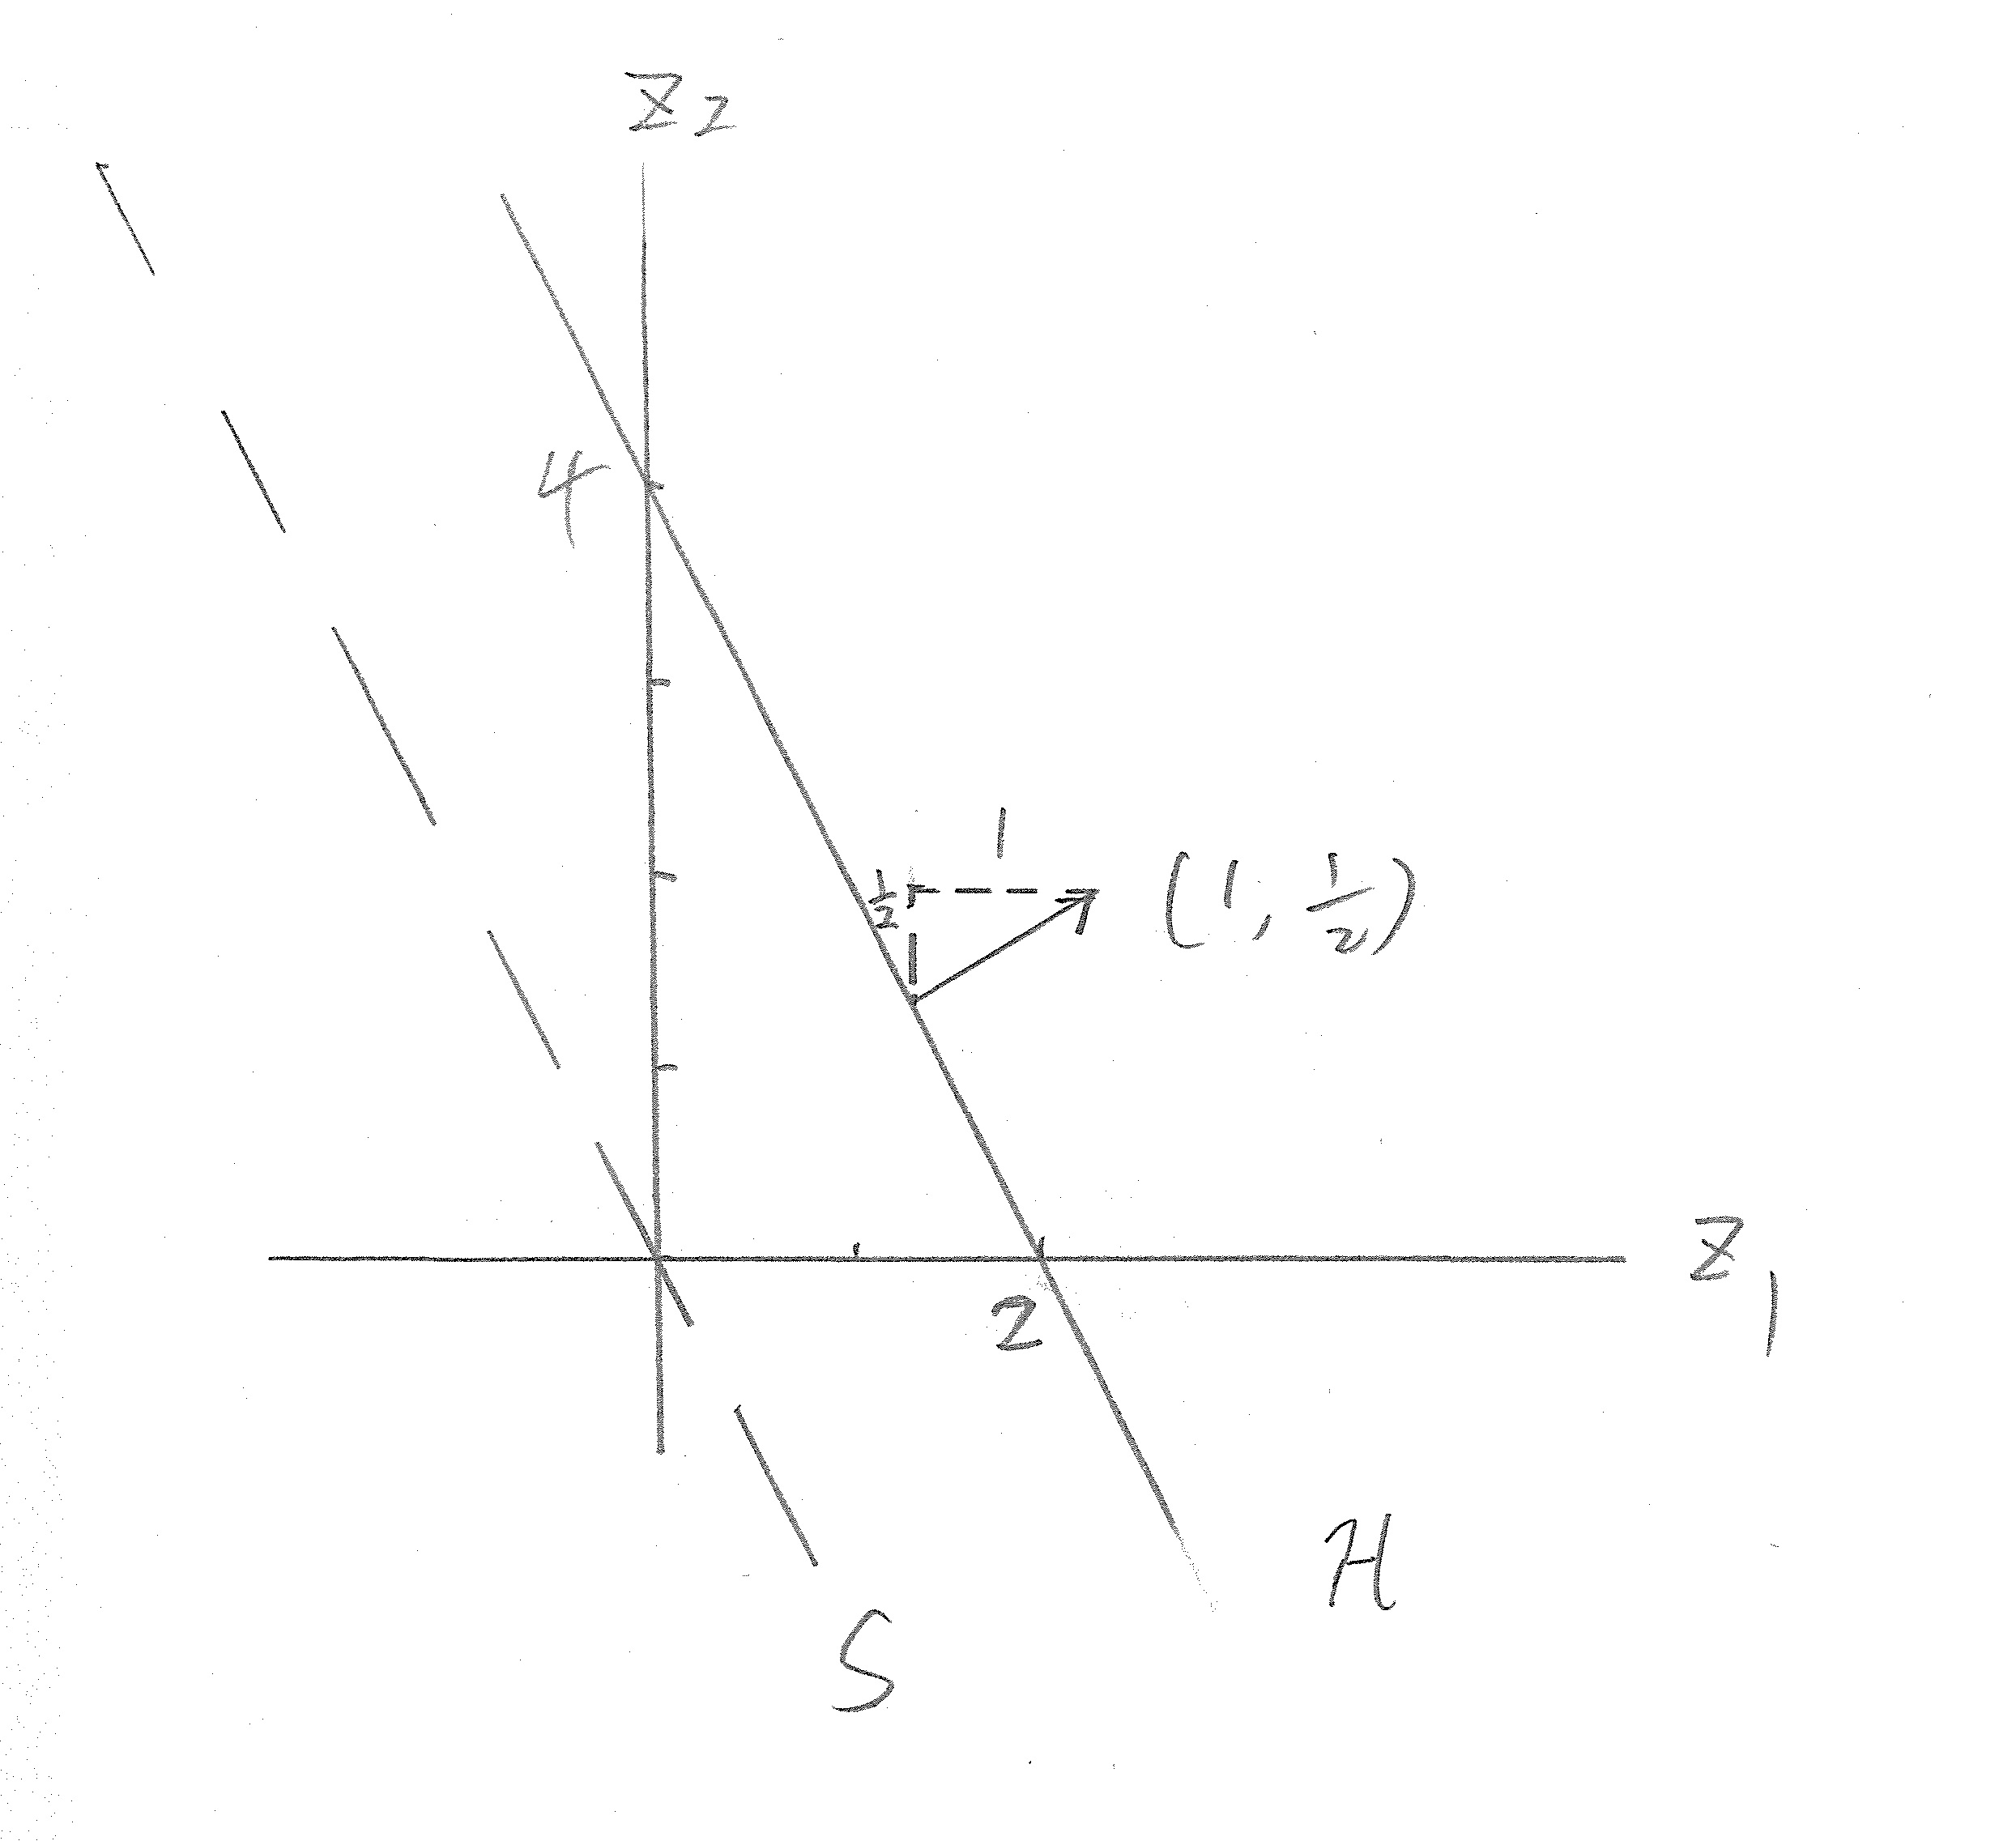
\includegraphics[width=2.1in,height=2.1in]{figures/ch02/p37.jpg}
	%\caption{This is an inserted JPG graphic} 
	%\label{fig:graph} 
\end{figure}


$\mathcal{H} = \{ z \in \mathbb{R}^n \vert z = u + z^{(0)}, u \in \mathcal{S}, z^{(0)} = \begin{bmatrix} 2\\ 0\\ \end{bmatrix} \}$

when 
\begin{align*}
\mathcal{S} &= \{z \in \mathbb{R}^2 | a^{T} z = 0 \} \\
&= \{z \in \mathbb{R}^2 | z_1 + \frac{1}{2} z_2 = 0 \}
\end{align*}

Note that recall any value at $z^{(0)} \in \mathcal{H}$ works so alternatively, e.g.,
$$\mathcal{H} = \{ z \in \mathbb{R}^n | z = u + z^{(0)}, u \in S, z^{(0)} = \begin{bmatrix} 0\\ 4\\ \end{bmatrix} \}$$
or 
$$\mathcal{H} = \{ z \in \mathbb{R}^n | z = u + z^{(0)}, u \in S, z^{(0)} = \begin{bmatrix} 1\\ 2\\ \end{bmatrix} \}\quad \text{, etc.} $$

\vspace{0.3cm}
Now let's back to the first example, projection onto hyperplane.
$$\mathcal{H}=\{z\in\reals^{n}\vert a^{\trans} z=b\}=\{z\in\reals^{n}|z=x_{s}+z^{(0)},x_{s}\in S, z^{(0)}\in \mathcal{H}\}$$

\begin{figure}
	\centering
	\resizebox{7.5cm}{3cm}{%% page 39

\def\RightAngle[size=#1](#2,#3,#4){%
 \draw ($(#3)!#1!(#2)$) -- 
       ($($(#3)!#1!(#2)$)!#1!90:(#2)$) --
       ($(#3)!#1!(#4)$);
 \path (#3) --
 ($($(#3)!#1!(#2)$)!#1!90:(#2)$);
}

\begin{tikzpicture}
\draw[thick,-stealth] (-3, 0) -- (3, 0);
\draw[thick,-stealth] (0, -2) -- (0, 4);

\coordinate (A) at (-3, -1.5);
\coordinate (B) at (3, 1.5);
\coordinate (C) at (-0.8, 1.1);
\draw (A) -- (B) node[right]{$\mathcal{S}$};

\coordinate (A1) at (-4, -0.5);
\coordinate (B1) at (3, 3);
\coordinate (C1) at (0.8, 3.4);
\draw (A1) -- (B1) node[right]{$\mathcal{A}$};

\coordinate (D1) at ($(A1)!(C1)!(B1)$);
\draw[dashed] (C1)node[above]{$p$} -- ($(A1)!(C1)!(B1)$)node[below right]{$p^{*}$};
%% right angle
\RightAngle[size=10pt](C1,D1,A1);

\end{tikzpicture}}
	\caption{}
	\label{}
\end{figure}

Recall that $\text{dim}(S)=n-1$, so $\text{dim}(S^{\perp})=1$, and we want to find the point $p^{*}=\arg \min_{p\in \mathcal{H}} \Vert p^{*}-p\Vert$.

Observe that $(p-p^{*}) \perp S$ (by optimal condition), So $(p-p^{*}) \in S^{\perp}=\{\lambda a|\lambda \in \reals \}$, and $\exists \lambda^{*}$ such that $p-p^{*}=\lambda^{*}a$.

Now, we want to solve for $\lambda^{*}$ but notice that there are 2 unknowns $(\lambda^{*},p^{*})$, and hence we get rid of $p^{*}$ dependency by using definition of $\mathcal{H}$.
\begin{align*}
&\qquad p-p^{*}=\lambda^{*}a\\
&\Leftrightarrow a^{\trans} (p-p^{*})=a^{\trans} (\lambda^{*}a)\\
&\Leftrightarrow a^{\trans} p-a^{\trans} p^{*}=\lambda^{*}a^{\trans} a\\
&\Leftrightarrow a^{\trans} p-b=\lambda^{*}a^{\trans} a\\
&\Leftrightarrow \lambda^{*}=\frac{a^{\trans} p-b}{a^{\trans} a}\\
&\Leftrightarrow \lambda^{*}=\frac{a^{\trans} p-b}{\Vert a\Vert^{2}}\\
\end{align*}

Thus, $p-p^{*}=\lambda^{*} a=(\frac{a^{\trans} p-b}{\Vert a\Vert^{2}})a$, or $p^{*}=p-(\frac{a^{\trans} p-b}{\Vert a\Vert^{2}})a$.

and 
$$\Vert p-p^{*}\Vert=\Vert \lambda^{*}a\Vert= \vert \lambda^{*}\vert \Vert a\Vert=\frac{\vert a^{\trans} p-b\vert}{\Vert a\Vert}$$.

Recall terminology $\Vert p-p^{*}\Vert=\min_{y\in \mathcal{H}} \Vert y-p\Vert$, we have
$$p^{*}=\arg\min_{y\in \mathcal{H}} \Vert y-p\Vert$$


\vspace{0.5cm}
\noindent\textbf{Projection w.r.t other norms}

Recall that inner product spaces have a notion of angle, have term "orthogonality principle", and the $L_{2}$ norm is one such example. In contrast, some norms such as $L_{1}$ and$ L_{\infty}$ norms don't come with a sense of angle. However the problem still make senses if $p\neq 2$, e.g., $p=1$, $p=\infty$, but we cannot apply $\perp$ principle since there is no sense of angle.

\vspace{0.3cm}
In following we will

(1). Discuss projection in normed vector spaces, particularly $L_{1}$ and $L_{\infty}$.

(2). Illustrate how the solution differs as you change the norm (change $p$).

(3). Give you a sense for character of difference such for $p=1$ and $p=\infty$.

(4). Get a sense of why might pick $p\neq 2$.

\newpage
Recall norm balls we draw before. Let's project $0\in\reals^{2}$ onto a line (affine set/hyperplane).

\begin{marginfigure}
	\centering
	\resizebox{7.5cm}{3cm}{%% page 42
%% fig 1
\begin{tikzpicture}
\draw[thick,-stealth] (-2, 0) -- (2, 0);
\draw[thick,-stealth] (0, -2) -- (0, 2);

\draw (0,0) circle [radius=1];
\node [below right] at (1, 0) { };

\end{tikzpicture}
}
	\caption{}
	\label{}
\end{marginfigure}

\begin{marginfigure}
	\centering
	\resizebox{7.5cm}{3cm}{%% page 42
%% fig 2
\begin{tikzpicture}
\draw[thick,-stealth] (-2, 0) -- (2, 0);
\draw[thick,-stealth] (0, -2) -- (0, 2);

\draw (-1, 0) -- (0, 1) -- (1, 0) -- (0, -1) -- (-1, 0);
\node [below right] at (1, 0) { };
\end{tikzpicture}
}
	\caption{}
	\label{}
\end{marginfigure}

\begin{marginfigure}
	\centering
	\resizebox{7.5cm}{3cm}{%% page 42
%% fig 3
\begin{tikzpicture}
\draw[thick,-stealth] (-2, 0) -- (2, 0);
\draw[thick,-stealth] (0, -2) -- (0, 2);

\draw (-1, -1) rectangle (1, 1);
\node [below right] at (1, 0) { };

\end{tikzpicture}

}
	\caption{}
	\label{}
\end{marginfigure}


\begin{figure}
	\centering
	\resizebox{7.5cm}{3cm}{%% page 42
%% fig 4
\begin{tikzpicture}
\draw[thick,-stealth] (-3, 0) -- (5, 0);
\draw[thick,-stealth] (0, -2) -- (0, 4);

\coordinate (O) at (0, 0) node[below right]{$O$};
\coordinate (A) at (-2, 2);
\coordinate (B) at (4.5, -1);
\draw (A) -- (B) node[right]{$\mathcal{A}$};
\end{tikzpicture}}
	\caption{}
	\label{}
\end{figure}

$$x^{*}=\arg\min_{x\in \mathcal{A}} \Vert x-0\Vert_{p}=\arg\min_{x\in \mathcal{A}} \Vert x\Vert_{p}$$


\begin{figure}
	\centering
	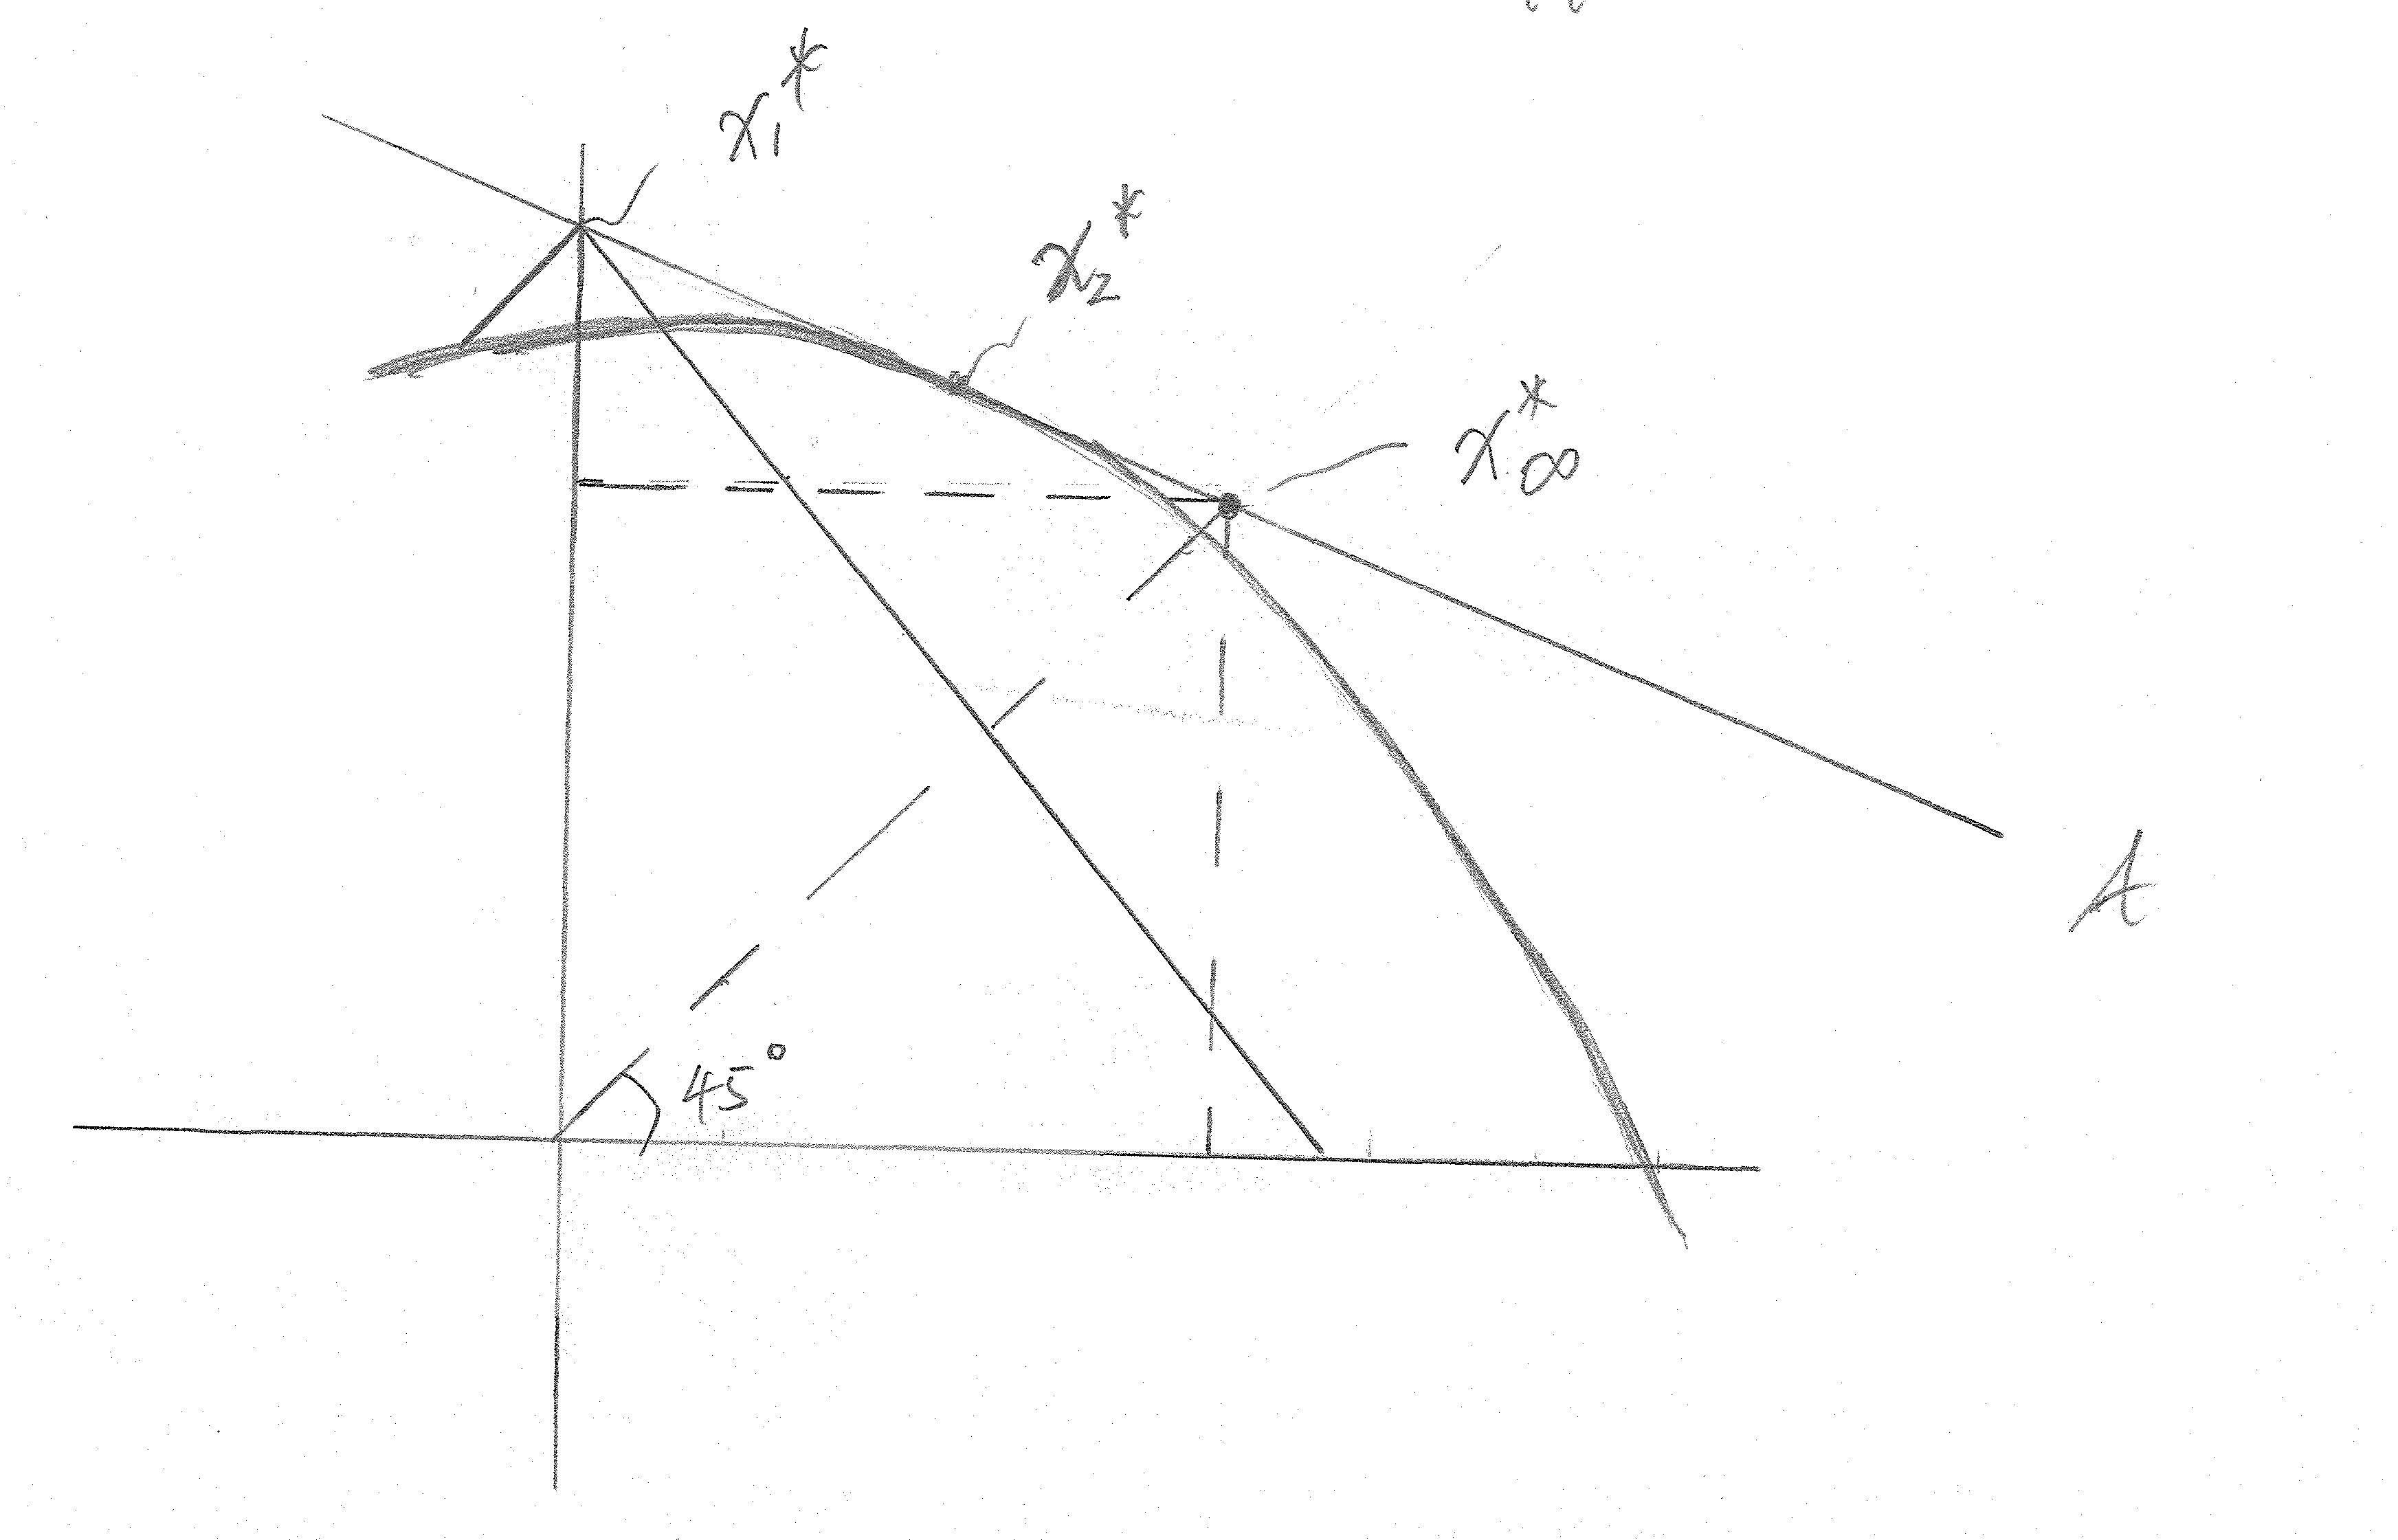
\includegraphics[width=2.1in,height=2.1in]{figures/ch02/p43.jpg}
	%\caption{This is an inserted JPG graphic} 
	%\label{fig:graph} 
\end{figure}


Observe that:

$x_{2}^{*}$: Familiar with solution via inner product and $\perp$ theorem, and has a closed form solution.

$x_{1}^{*}$: Solution is "sparse", generally will be the case for affine constraints since vertices of norm-ball are axis-aligned.

$x_{\infty}^{*}$: At optimum, $x_{\infty, 1}^{*}=x_{\infty, 2}^{*}$, equal-magnitude coordinate.


\vspace{0.5cm}
\noindent\textbf{Functions}

Some terminologies will be used in this material:

"Function":  $F:\reals^{n}\mapsto \reals$

"Map":  $F:\reals^{n}\mapsto \reals^{m}$


However, not all input values may be allowed, input may be a subset of $\Omega$ (cf, $\reals^{n}$), this is the "domain" of $F$.% that is
%$$\text{dom} F= \{x\in\reals^{n}|\vert F(x)\vert\leq\infty\}$$

\vspace{0.5cm}
Aside: Terminology when discussion a pair of vector space $(\cal{V},\cal{U})$ over a field $\mathbb{F}$

$F:\cal{U}\mapsto \cal{V}$, a "map", generally $\text{dim}(\cal{U})\neq \text{dim}(\cal{V})$.

$F:\cal{U}\mapsto \cal{U}$ , an "operator", input and output vectors spaces have the same dimension.

$F:\cal{U}\mapsto \mathbb{F}$ , a "functional", map vector space into a scalar.

In this course, $\cal{U}$=$\reals^{n}$, $\cal{V}$=$\reals^{m}$, $\mathbb{F}$=$\reals$ (or, occasionally $\complex$).


\vspace{0.3cm}
\textbf{Sets related to functions}

Various sets defined by a function tell us a lot(or sometimes everything) about a function $F:\reals^{n}\mapsto\reals$

(1) The "graph" (a.k.a, "plot") of $F$ is the set
$$F=\{(x,F(x))\in\reals^{n+1}:x\in\reals^{n}\}$$

(2) The "epigraph" of $F$ is the set 
$$F=\{(x,t)\in\reals^{n+1}:x\in\reals^{n}, t\geq F(x) \}$$

\begin{marginfigure}
	\centering
	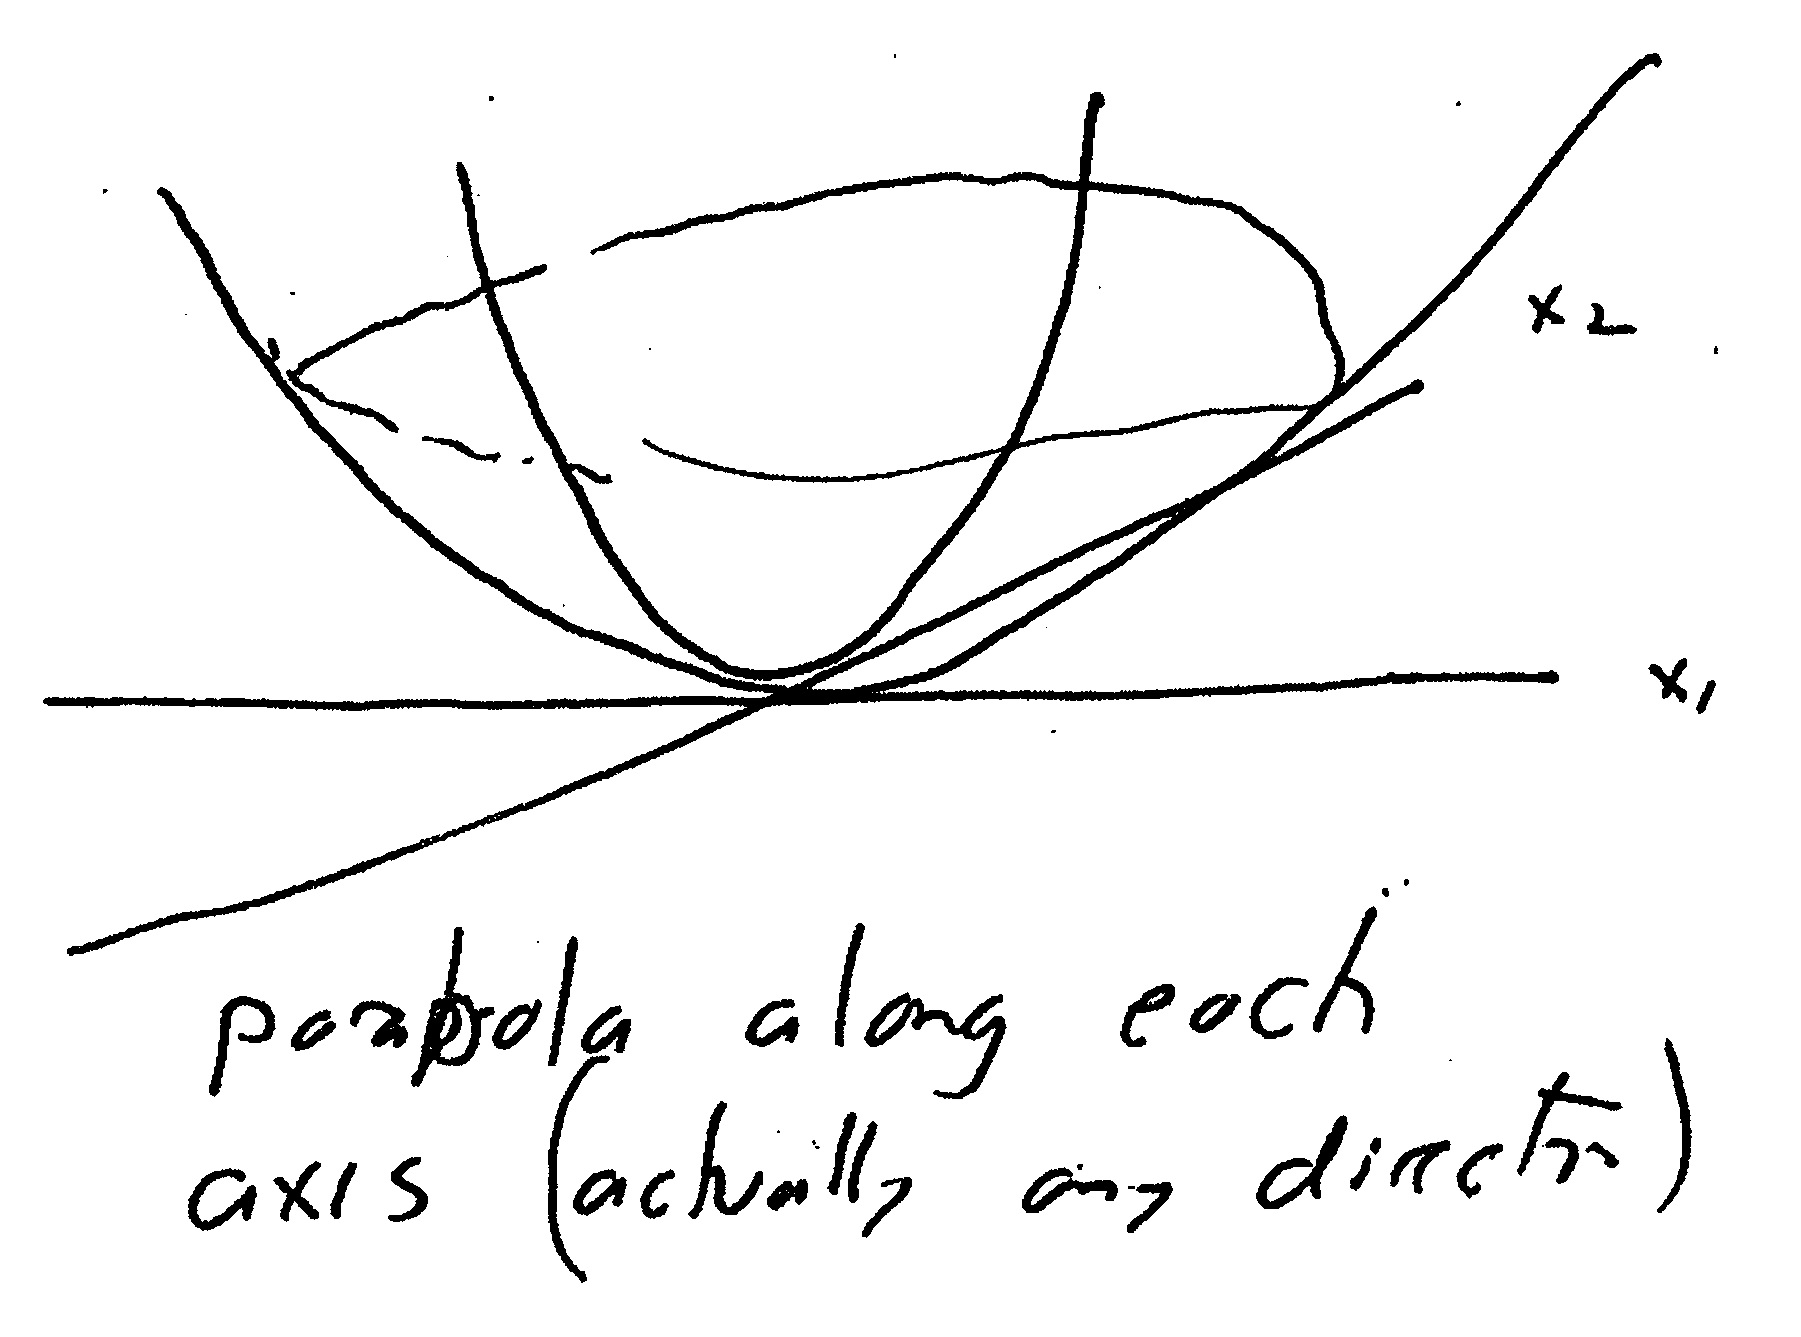
\includegraphics[width=2.1in,height=2.1in]{figures/ch02/p48-1.jpg}
	\caption{Graph 1} 
	%\label{fig:graph} 
\end{marginfigure}

\begin{marginfigure}
	\centering
	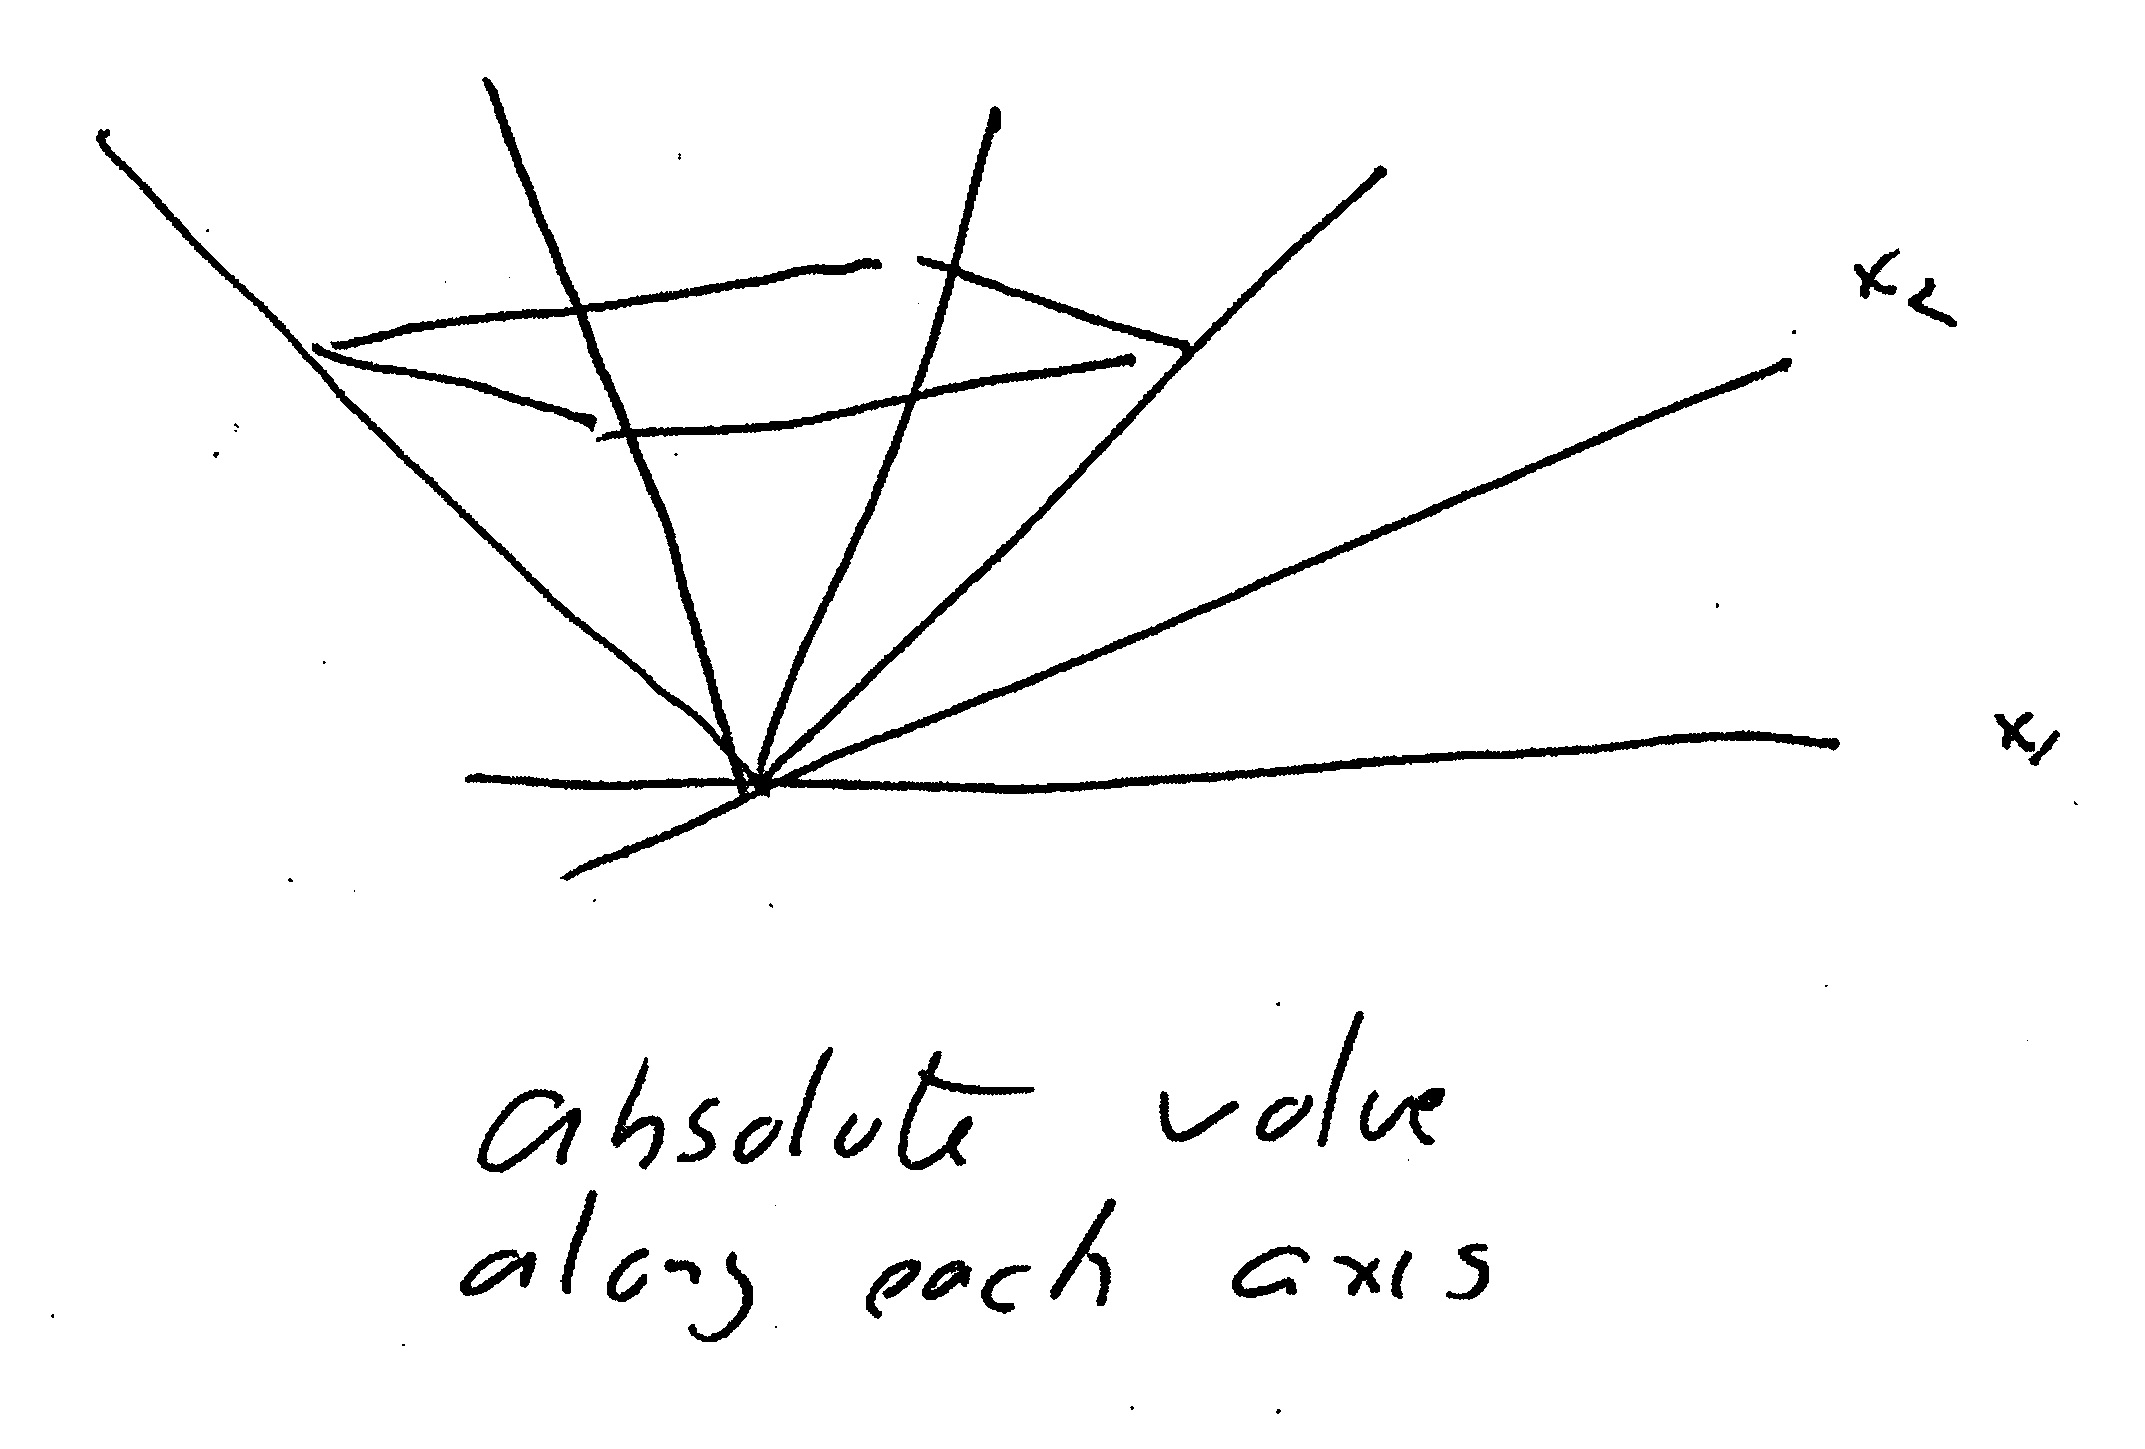
\includegraphics[width=2.1in,height=2.1in]{figures/ch02/p48-2.jpg}
	\caption{Graph 2} 
	%\label{fig:graph} 
\end{marginfigure}

\begin{marginfigure}
	\centering
	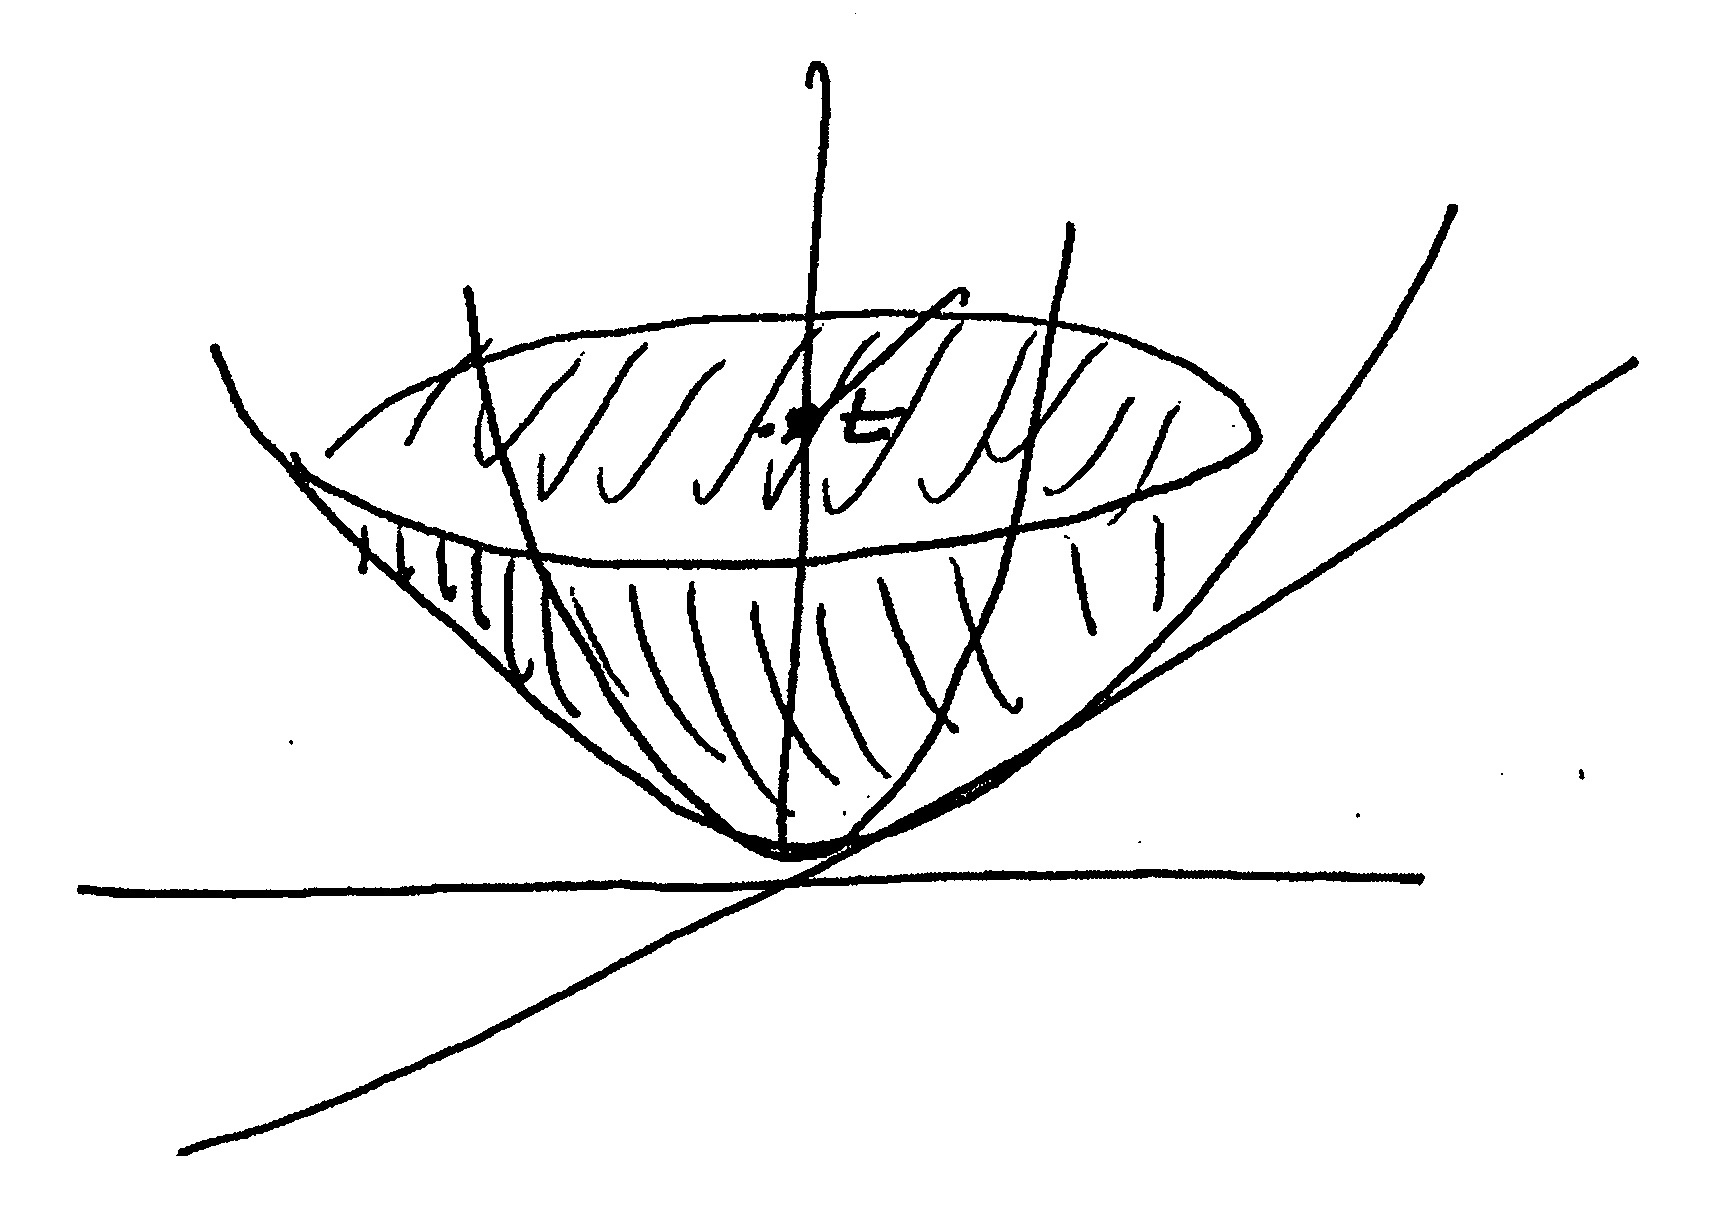
\includegraphics[width=2.1in,height=2.1in]{figures/ch02/p48-3.jpg}
	\caption{Epigraph 1} 
	%\label{fig:graph} 
\end{marginfigure}

\begin{marginfigure}
	\centering
	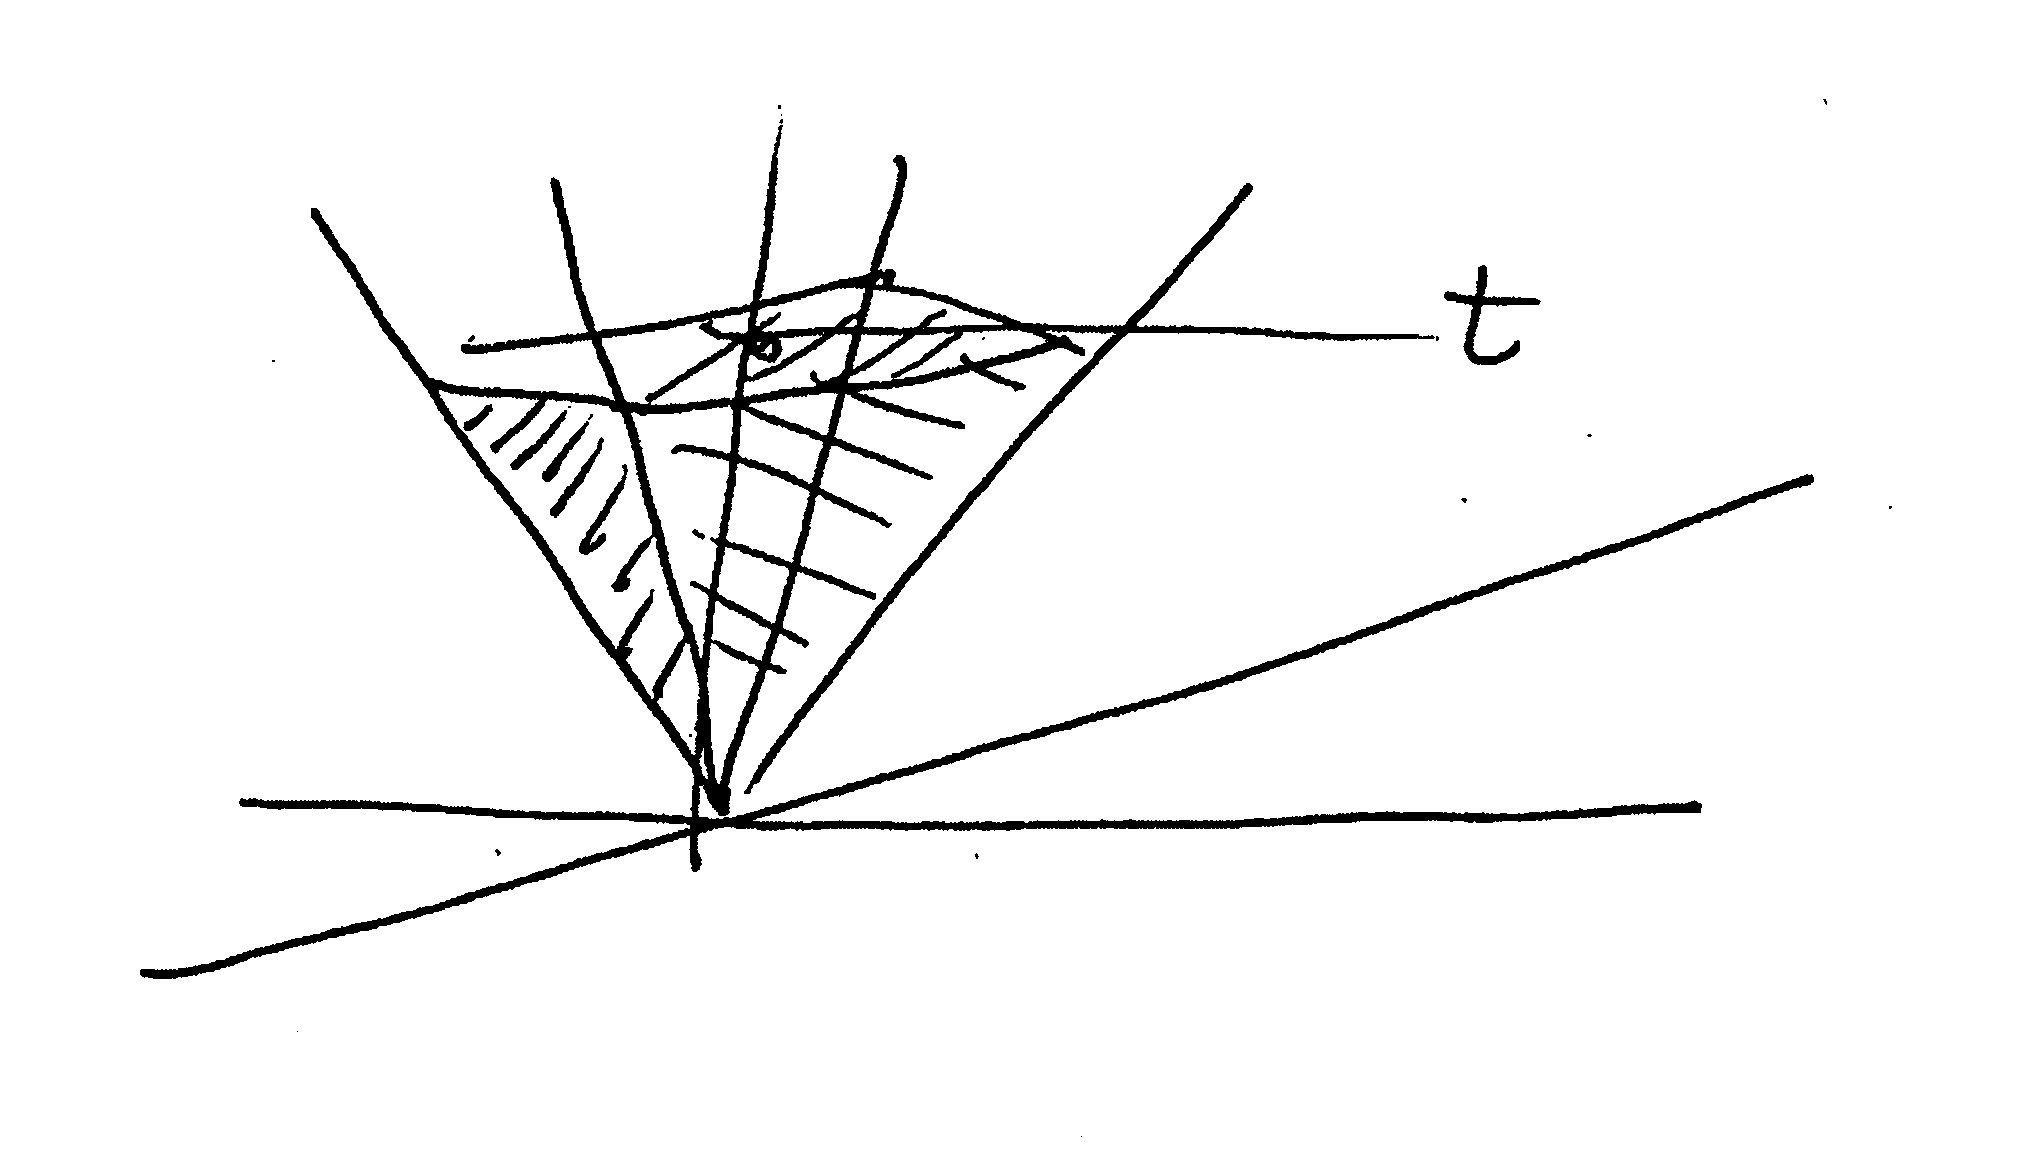
\includegraphics[width=2.1in,height=2.1in]{figures/ch02/p48-4.jpg}
	\caption{Epigraph 2} 
	%\label{fig:graph} 
\end{marginfigure}


Graph
\begin{figure}
	\centering
	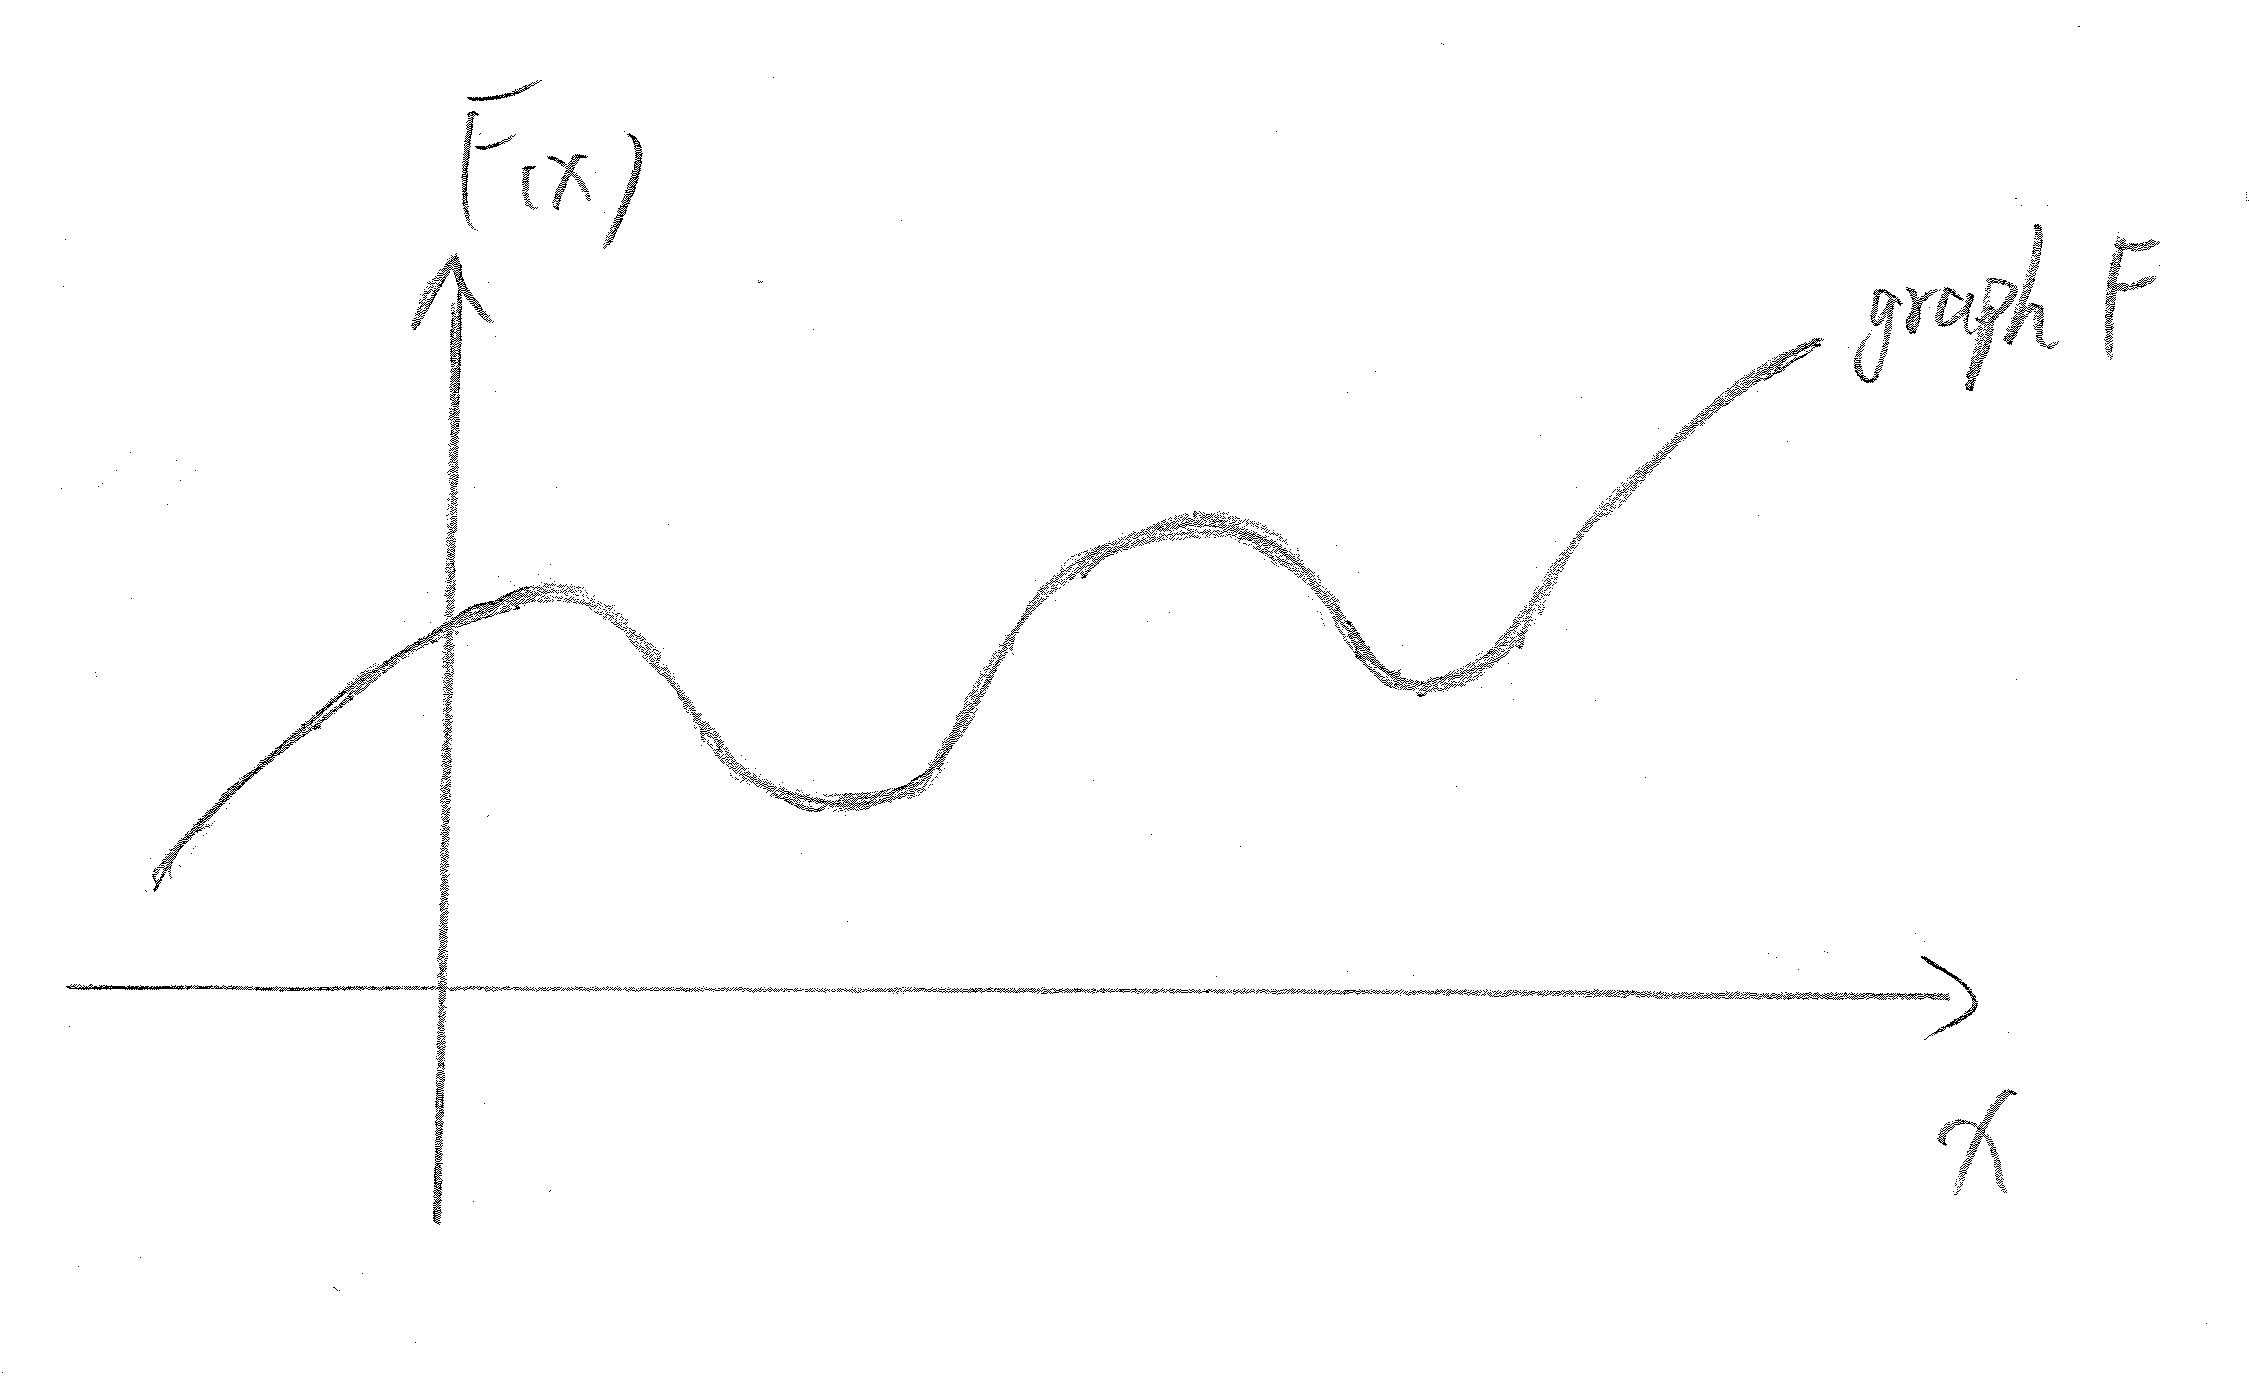
\includegraphics[width=2.1in,height=2.1in]{figures/ch02/p47-1.jpg}
	%\caption{This is an inserted JPG graphic} 
	\label{fig:graph} 
\end{figure}

Epigraph
\begin{figure}
	\centering
	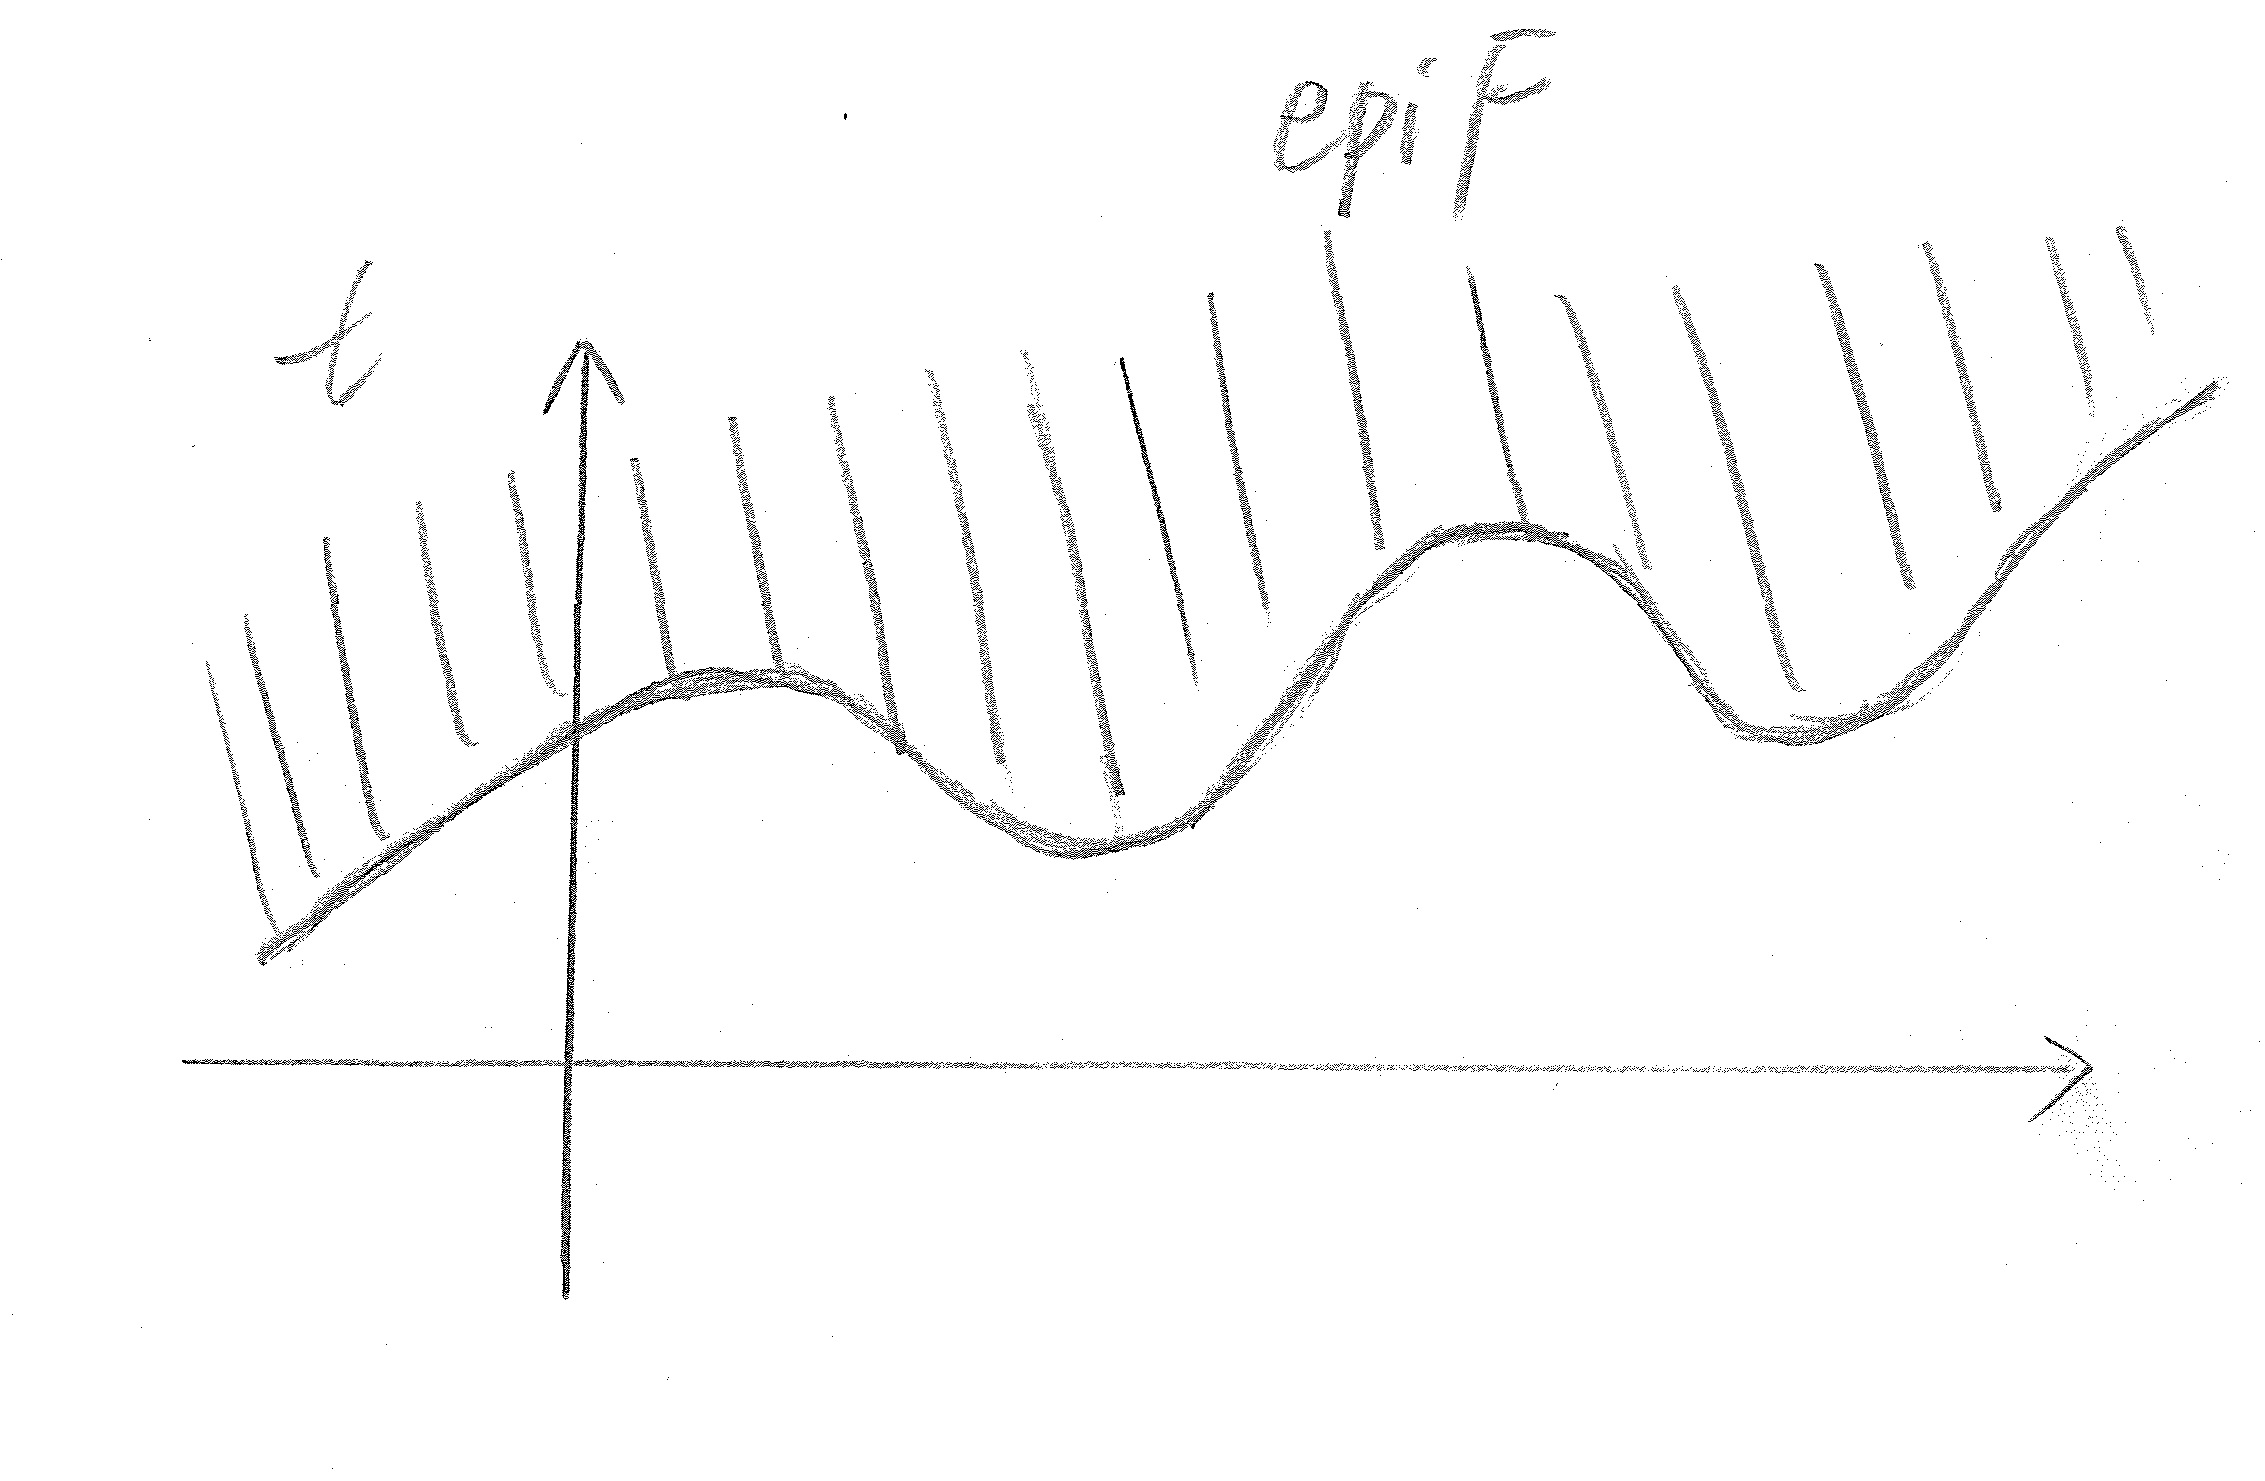
\includegraphics[width=2.1in,height=2.1in]{figures/ch02/p47-2.jpg}
	%\caption{This is an inserted JPG graphic} 
	%\label{fig:graph} 
\end{figure}



It is also useful to consider points at(or below) a height

(3) The "level" set
$$c_{F}(t)=\{x\in\reals^{n}:F(x)=t\}$$

(4) The "sub-level" set
$$L_{F}(t)=\{x\in\reals^{n}:F(x)\leq t\}$$

Note: graph and epigraph are in $\reals^{n+1}$, level and sublevel set are in $\reals^{n}$


\vspace{0.5cm}
Let's sketch these sets for $L_{2}$ and $L_{1}$ norms in $\reals^{2}$ on the r.h.s.

\newpage

\begin{marginfigure}
	\centering
	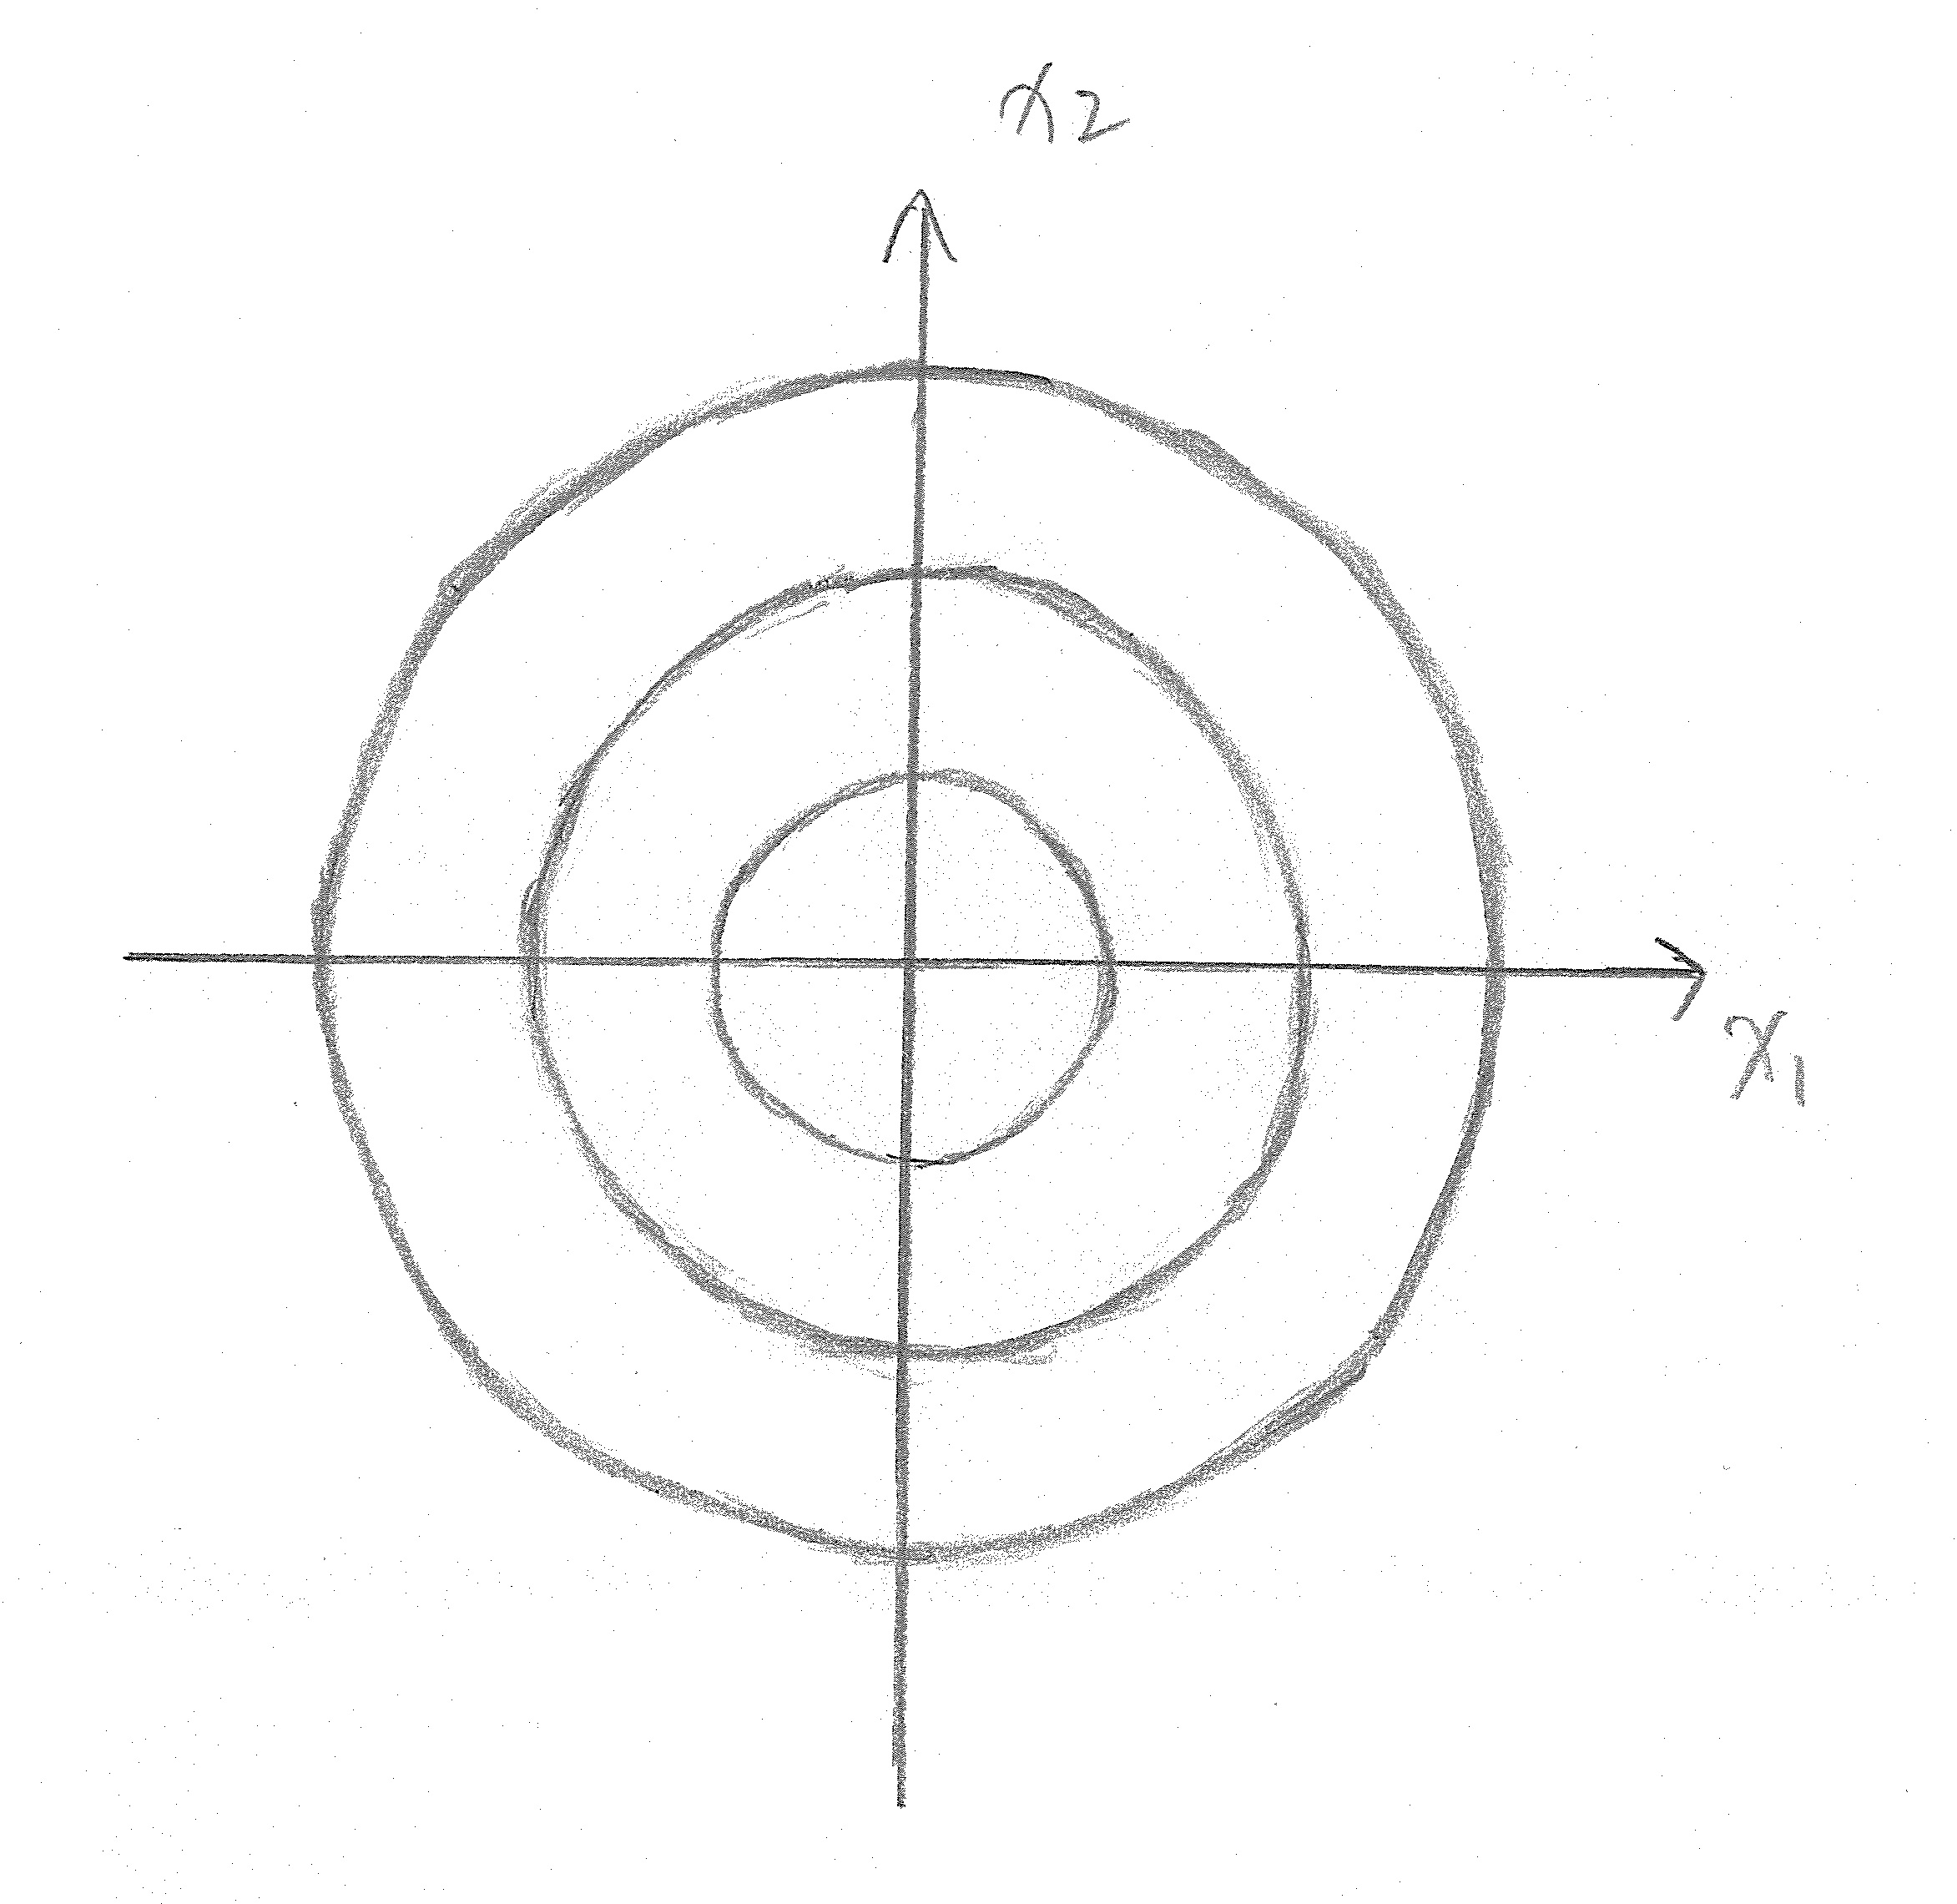
\includegraphics[width=2.1in,height=2.1in]{figures/ch02/p48-5.jpg}
		\caption{Level set 1} 
	%\label{fig:graph} 
\end{marginfigure}

\begin{marginfigure}
	\centering
	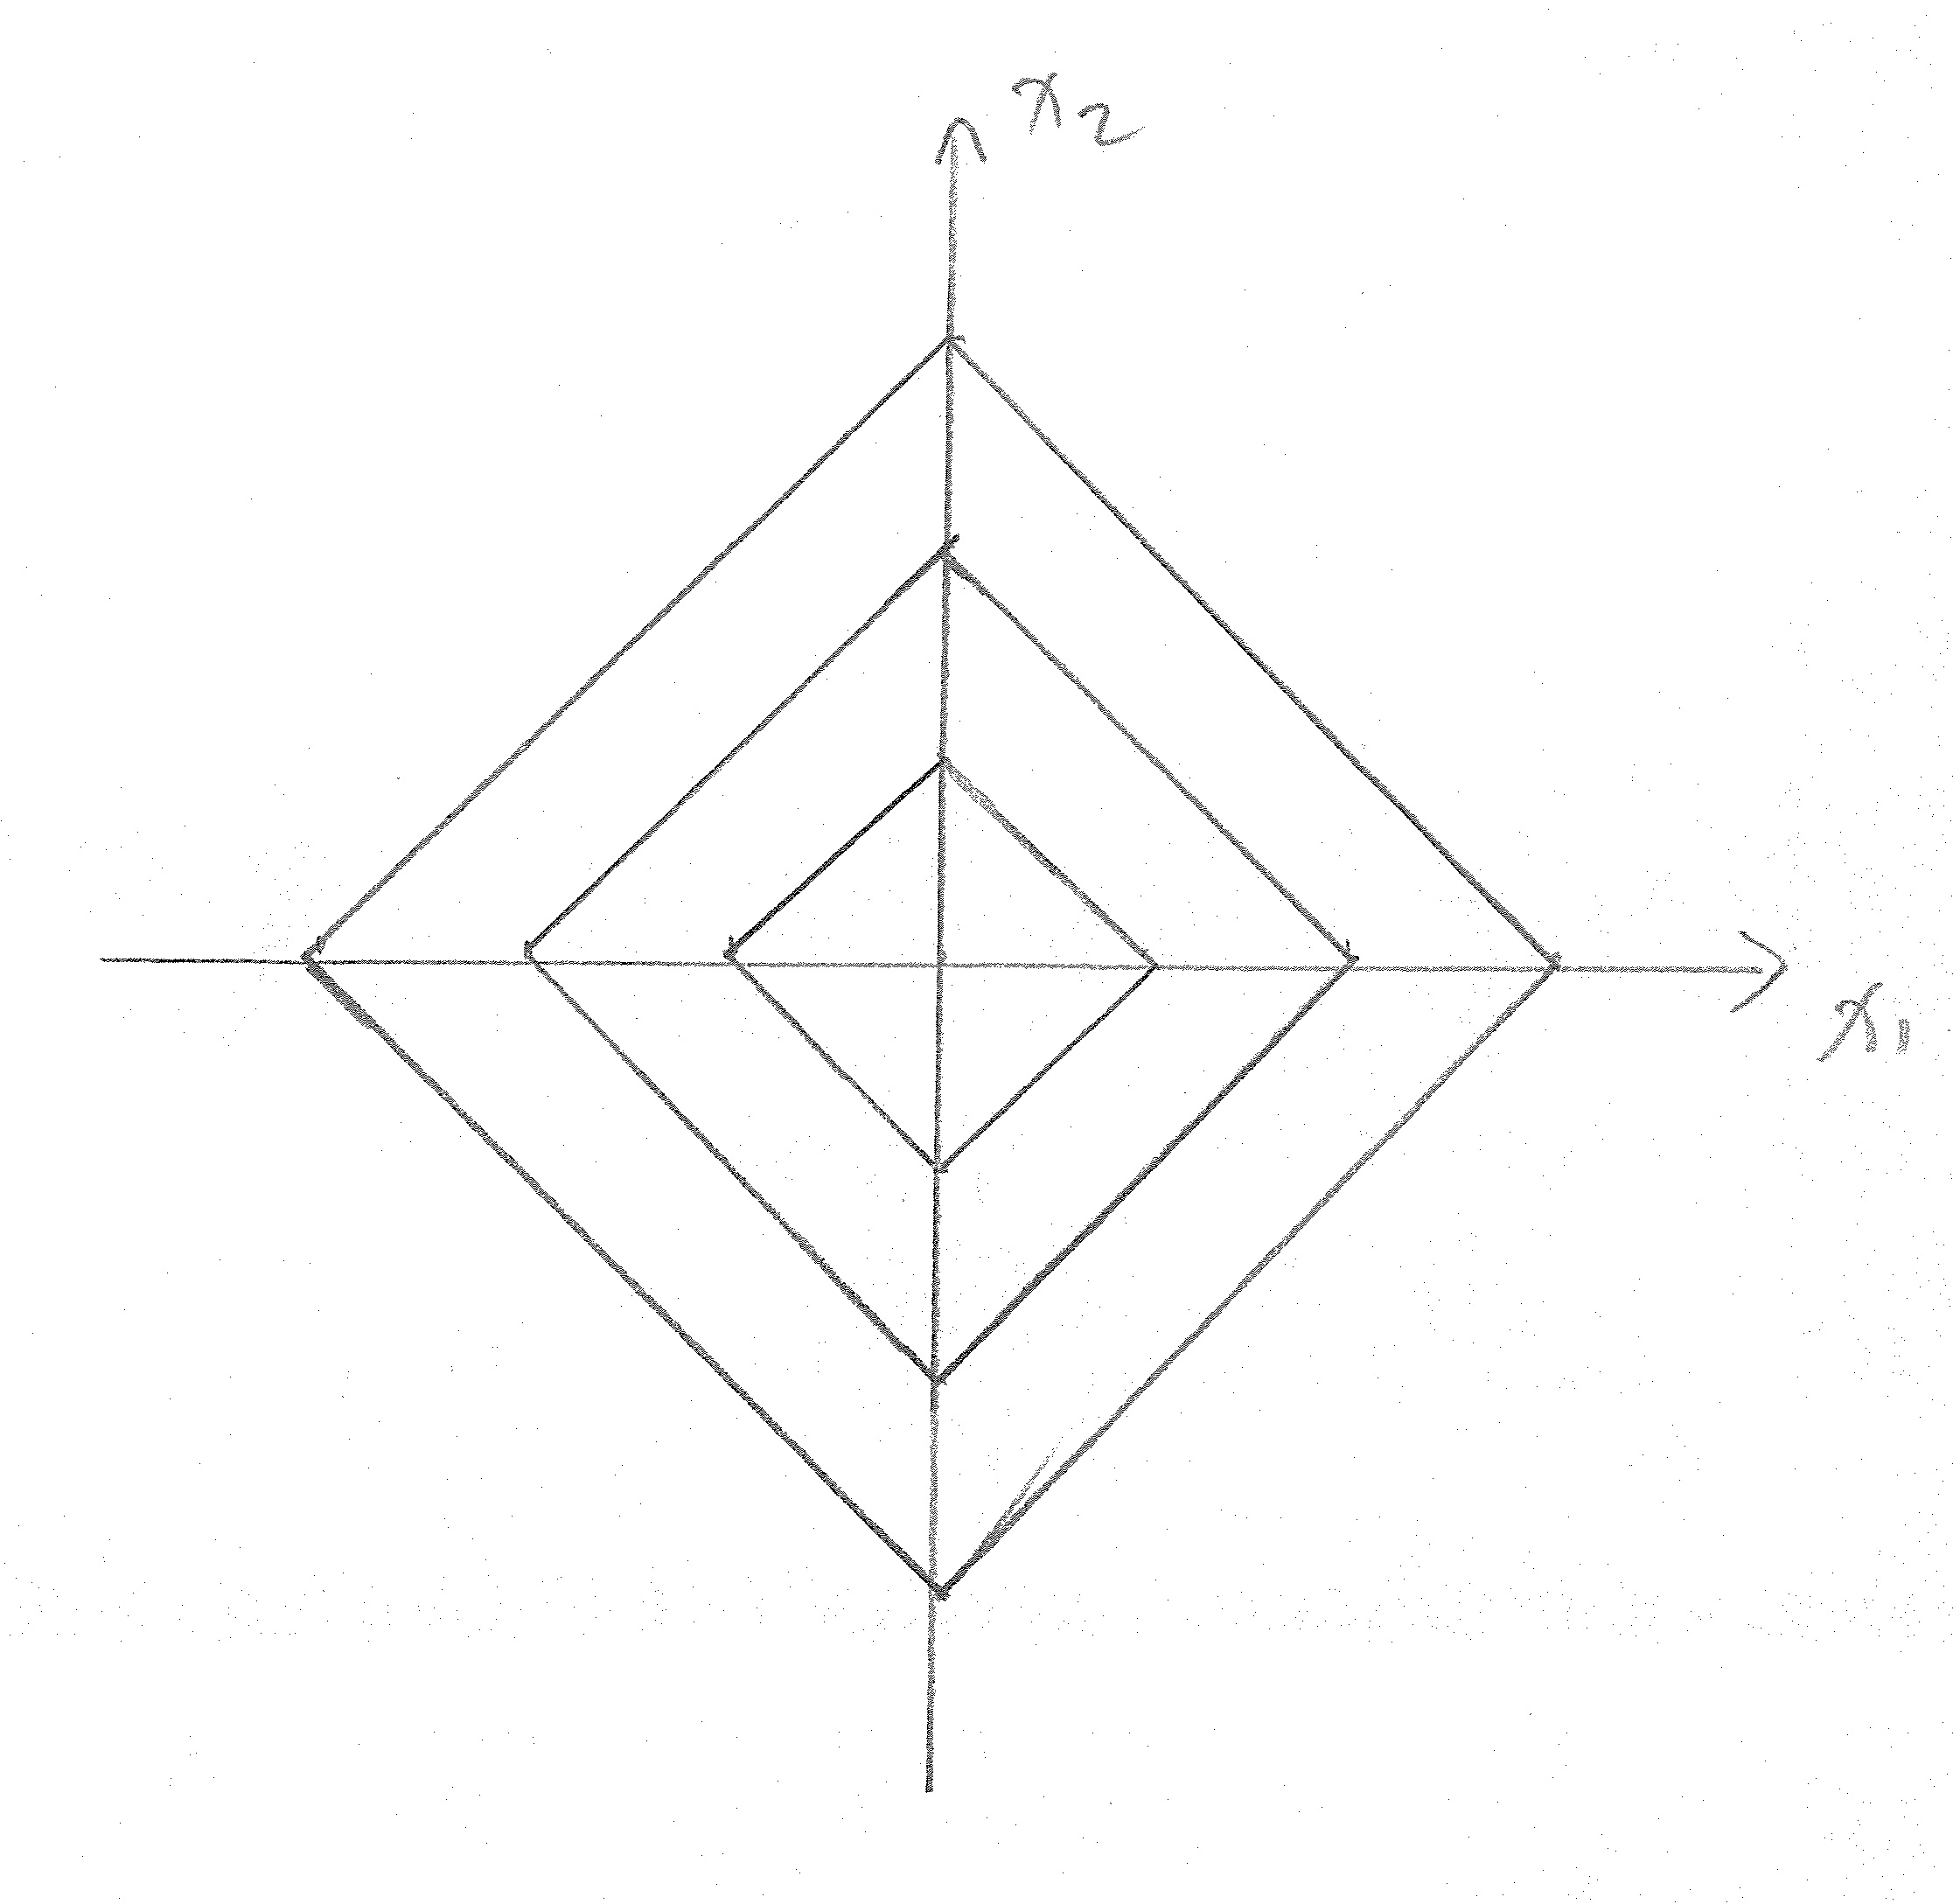
\includegraphics[width=2.1in,height=2.1in]{figures/ch02/p48-6.jpg}
	\caption{Level set 2} 
	%\label{fig:graph} 
\end{marginfigure}

\begin{marginfigure}
	\centering
	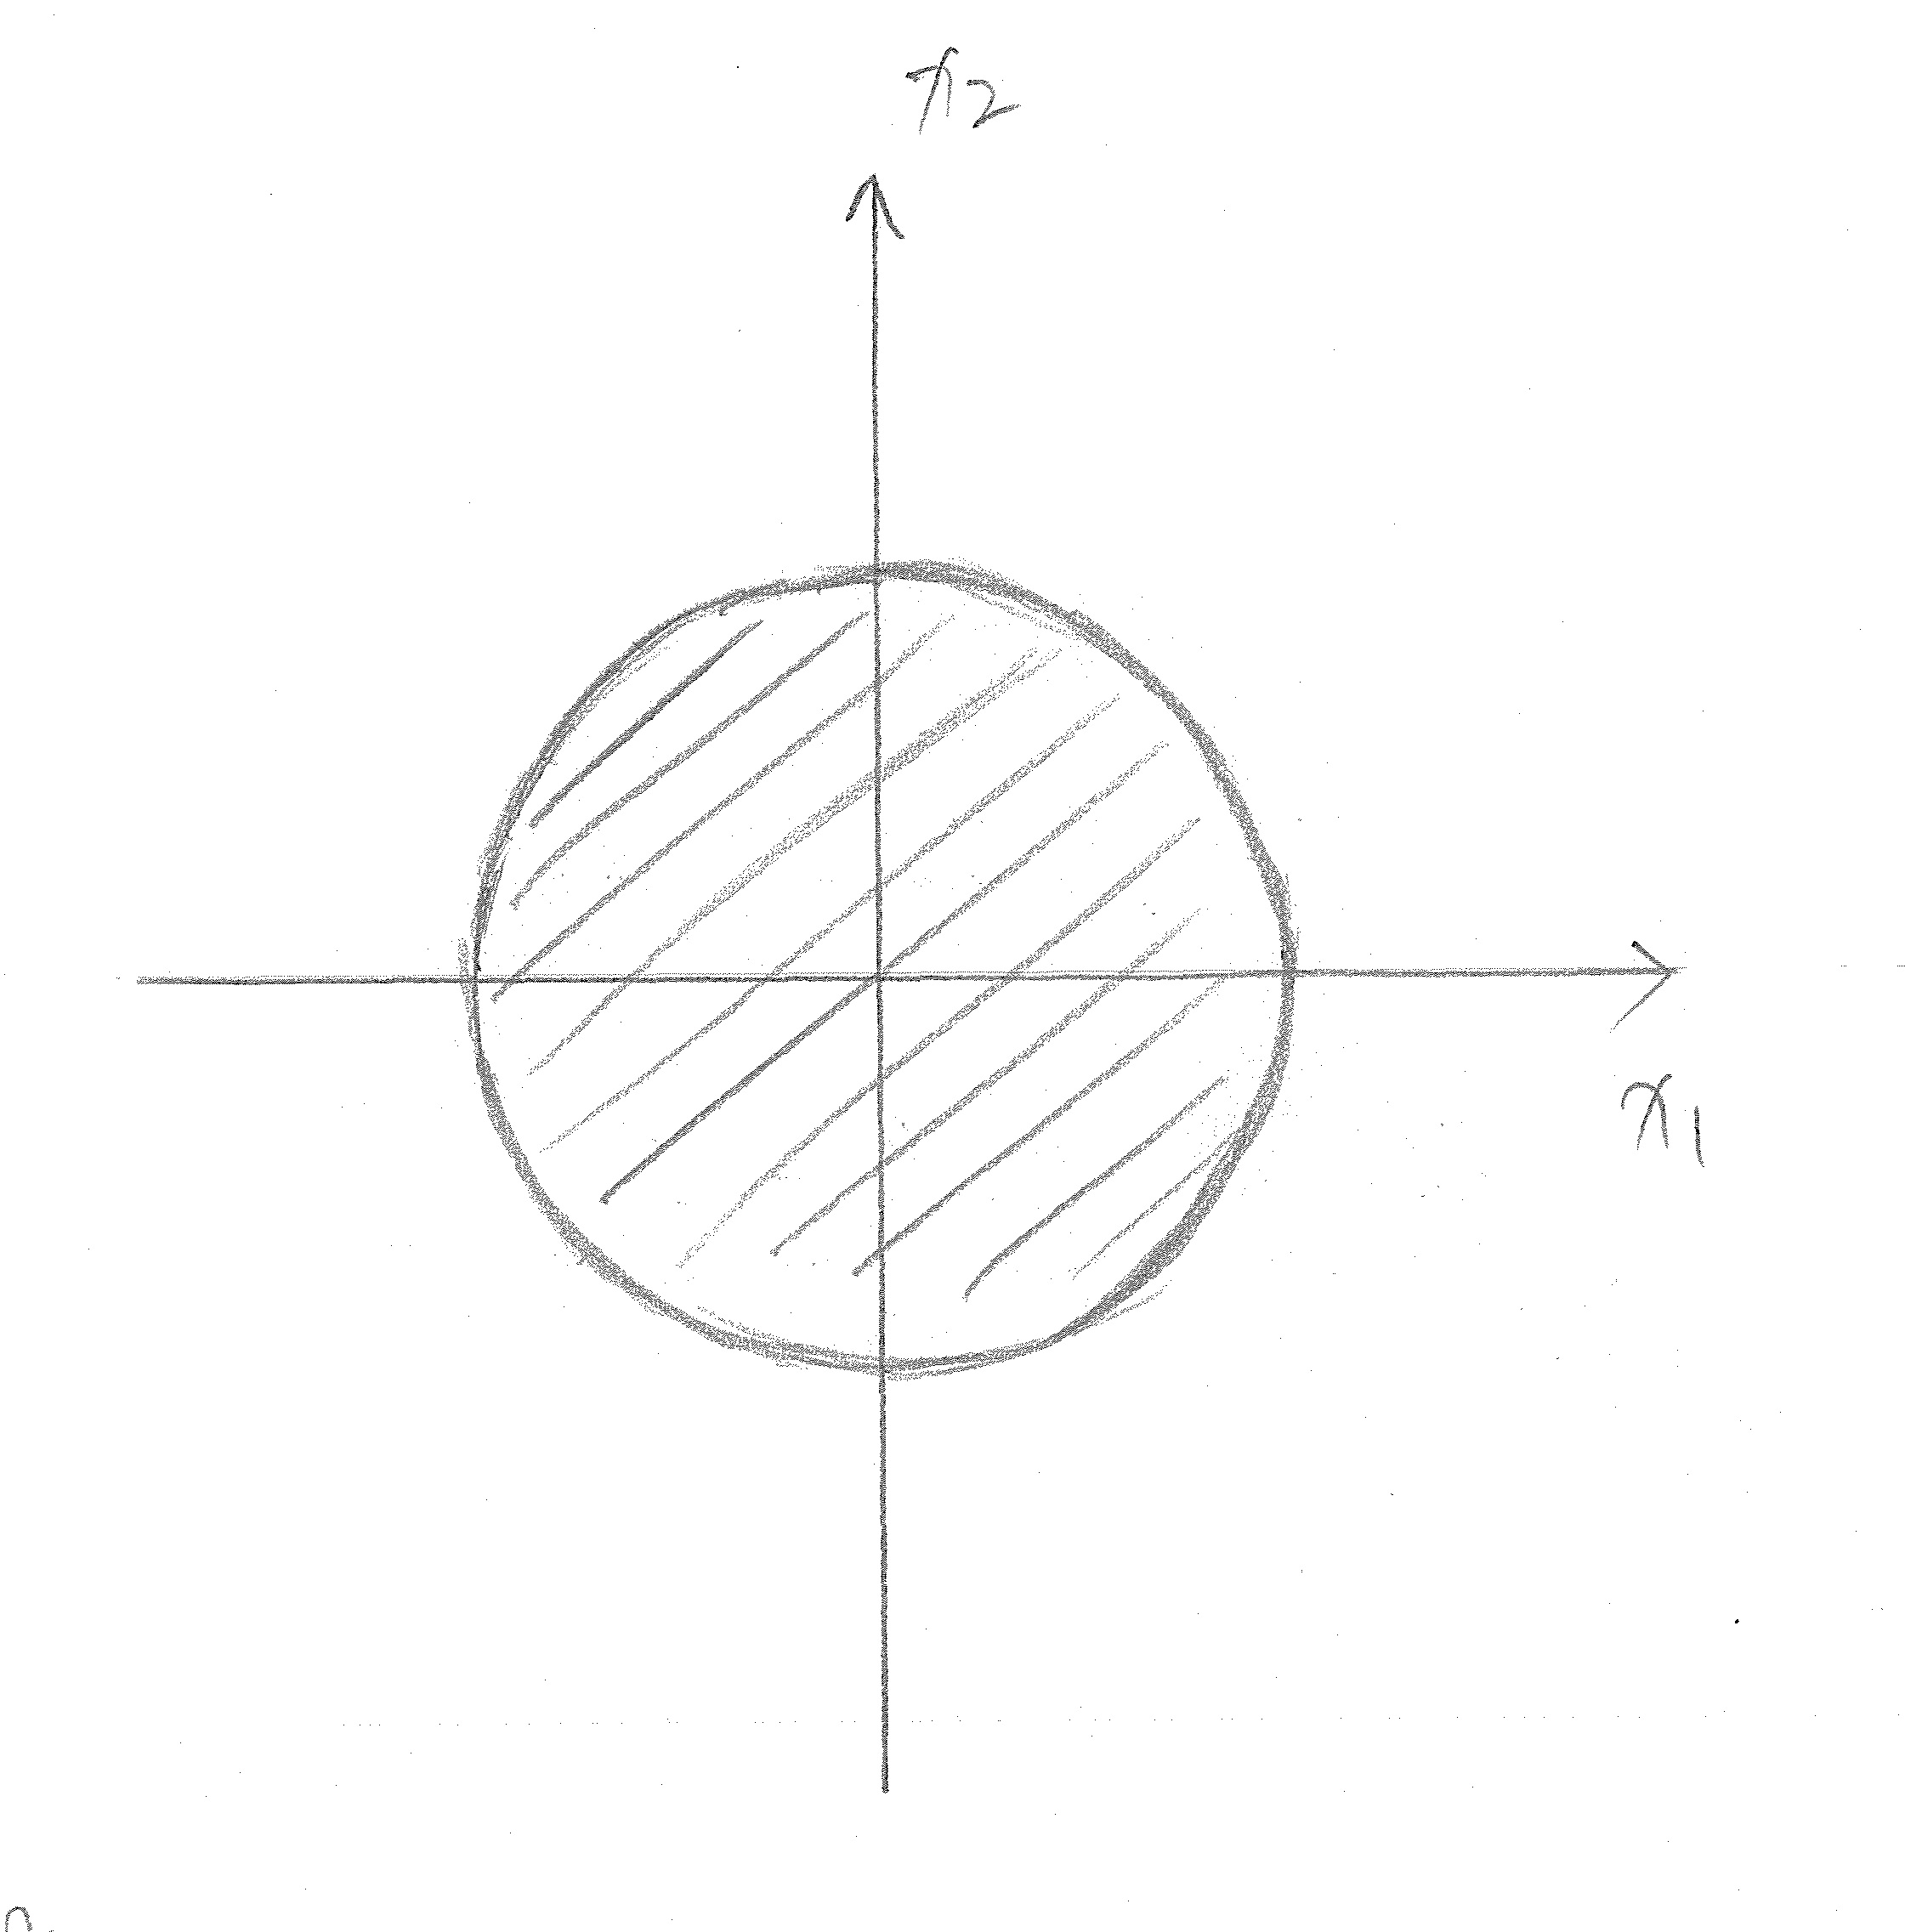
\includegraphics[width=2.1in,height=2.1in]{figures/ch02/p48-7.jpg}
	\caption{Sub-level set 1} 
	%\label{fig:graph} 
\end{marginfigure}

\begin{marginfigure}
	\centering
	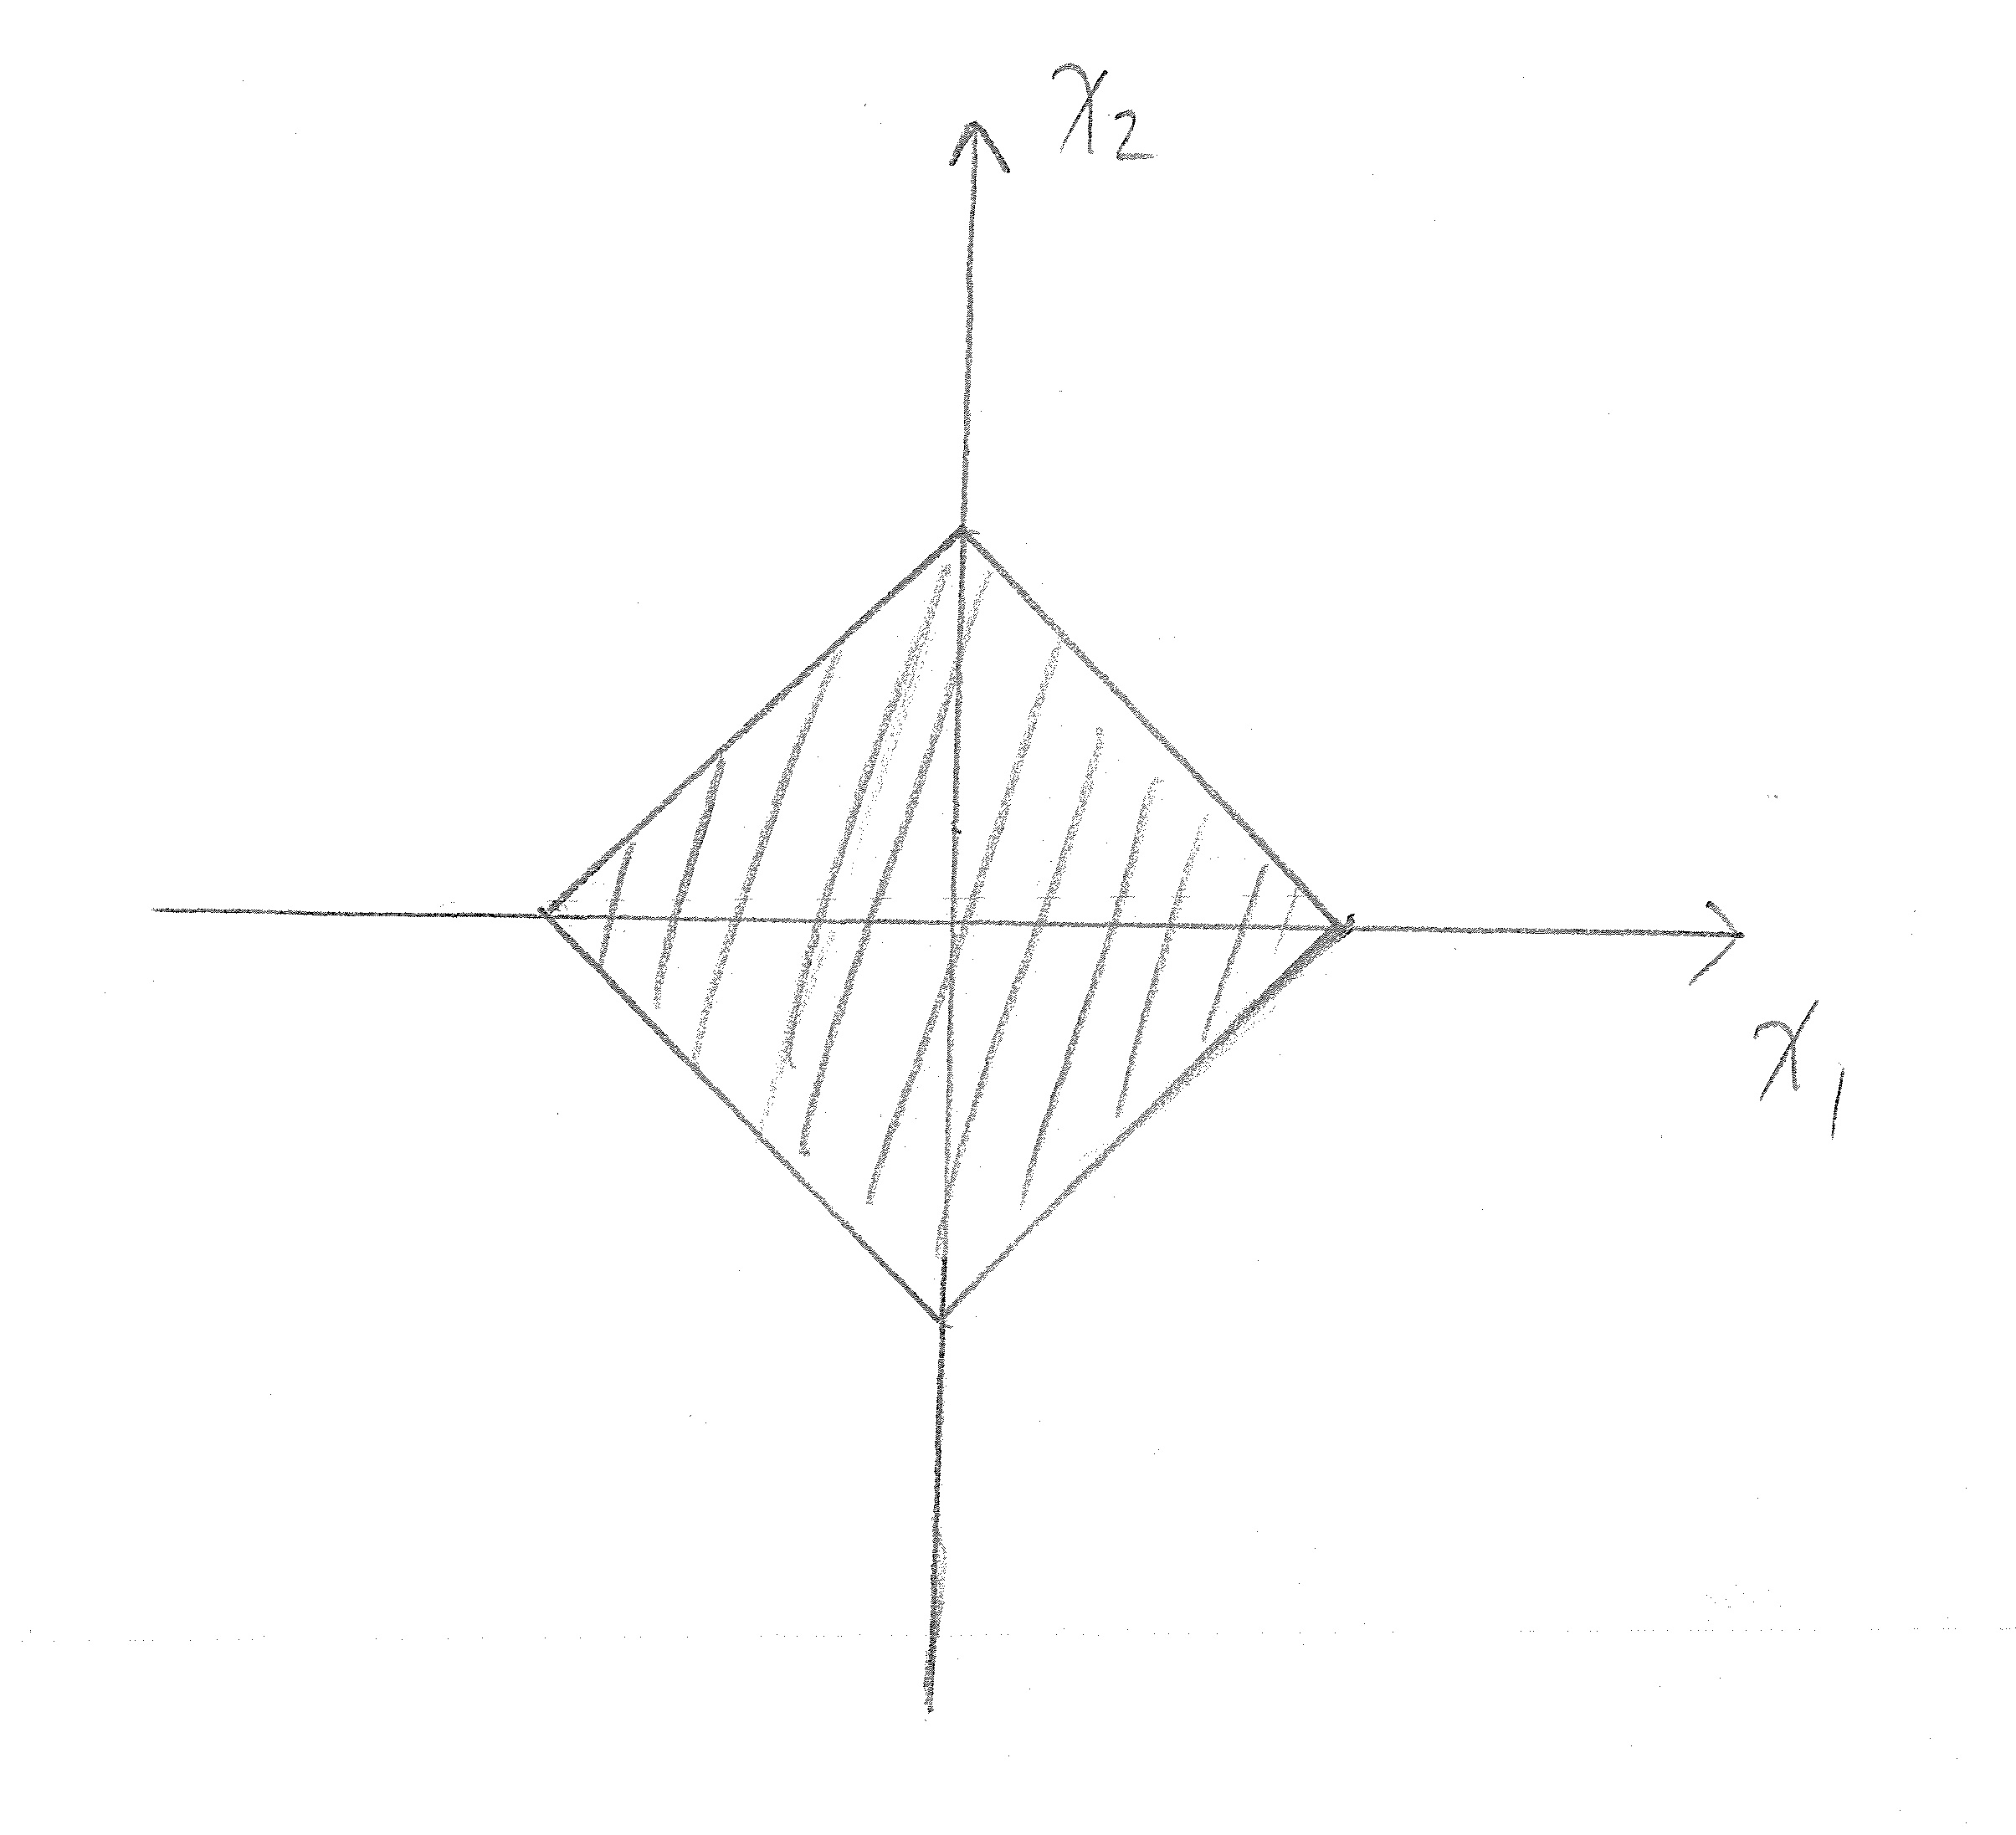
\includegraphics[width=2.1in,height=2.1in]{figures/ch02/p48-8.jpg}
	\caption{Sub-level set 2} 
	%\label{fig:graph} 
\end{marginfigure}

\vspace{0.5cm}
\textbf{Linear and affine functions}

1. A function $F:\reals^{n}\mapsto\reals$ is linear iff following two properties are satisfied

(1) "Homogeneous": $F(ax)=aF(x)$,$ \forall x\in\reals^{n}$ and $a\in\reals$

(2) "Additivity":  $F(x^{(1)}+x^{(2)})=F(x^{(1)})+F(x^{(2)})$

Put together to get 
$$F(\sum_{i\in [d]}^{}a_{i}x^{(i)})=\sum_{i\in [d]}^{}a_{i}F(x^{(i)})$$

\vspace{0.3cm}
2. A function $F:\reals^{n}\mapsto\reals$ is affine iff

Let $\overline{F}$ define pointwise as $\overline{F}=F(x)-F(0)$, $\forall x\in\reals^{n}$ is a linear function. The $F:\reals^{n}\mapsto\reals$ is affine iff there is a unique pair $(a,b)\in\reals^{n}\times\reals$ such that 
$$F(x)=a^{\trans} x+b,\  \forall x\in\reals^{n}$$

Since $F(0)=b$, this implies that any linear function can be expressed as $F(x)=a^{\trans} x=\langle a,x\rangle$ for some unique $a\in\reals^{n}$.

\vspace{0.5cm}
\textbf{Sets and linear/affine functions}

The graph of $F:\reals^{n}\mapsto\reals$ is a 

\quad- subspace of $\reals^{n+1}$ if $F$ is linear.

\quad- hyperplane of $\reals^{n+1}$ if $F$ is affine.

\vspace{0.2cm}
The epigraph of $F:\reals^{n}\mapsto\reals$ is a 

\quad- half-space of $\reals^{n+1}$ if $F$ is affine.

\quad- half-space the boarder at which includes $0\in\reals^{n+1}$ if $F$ is linear.


\begin{figure}
	\centering
	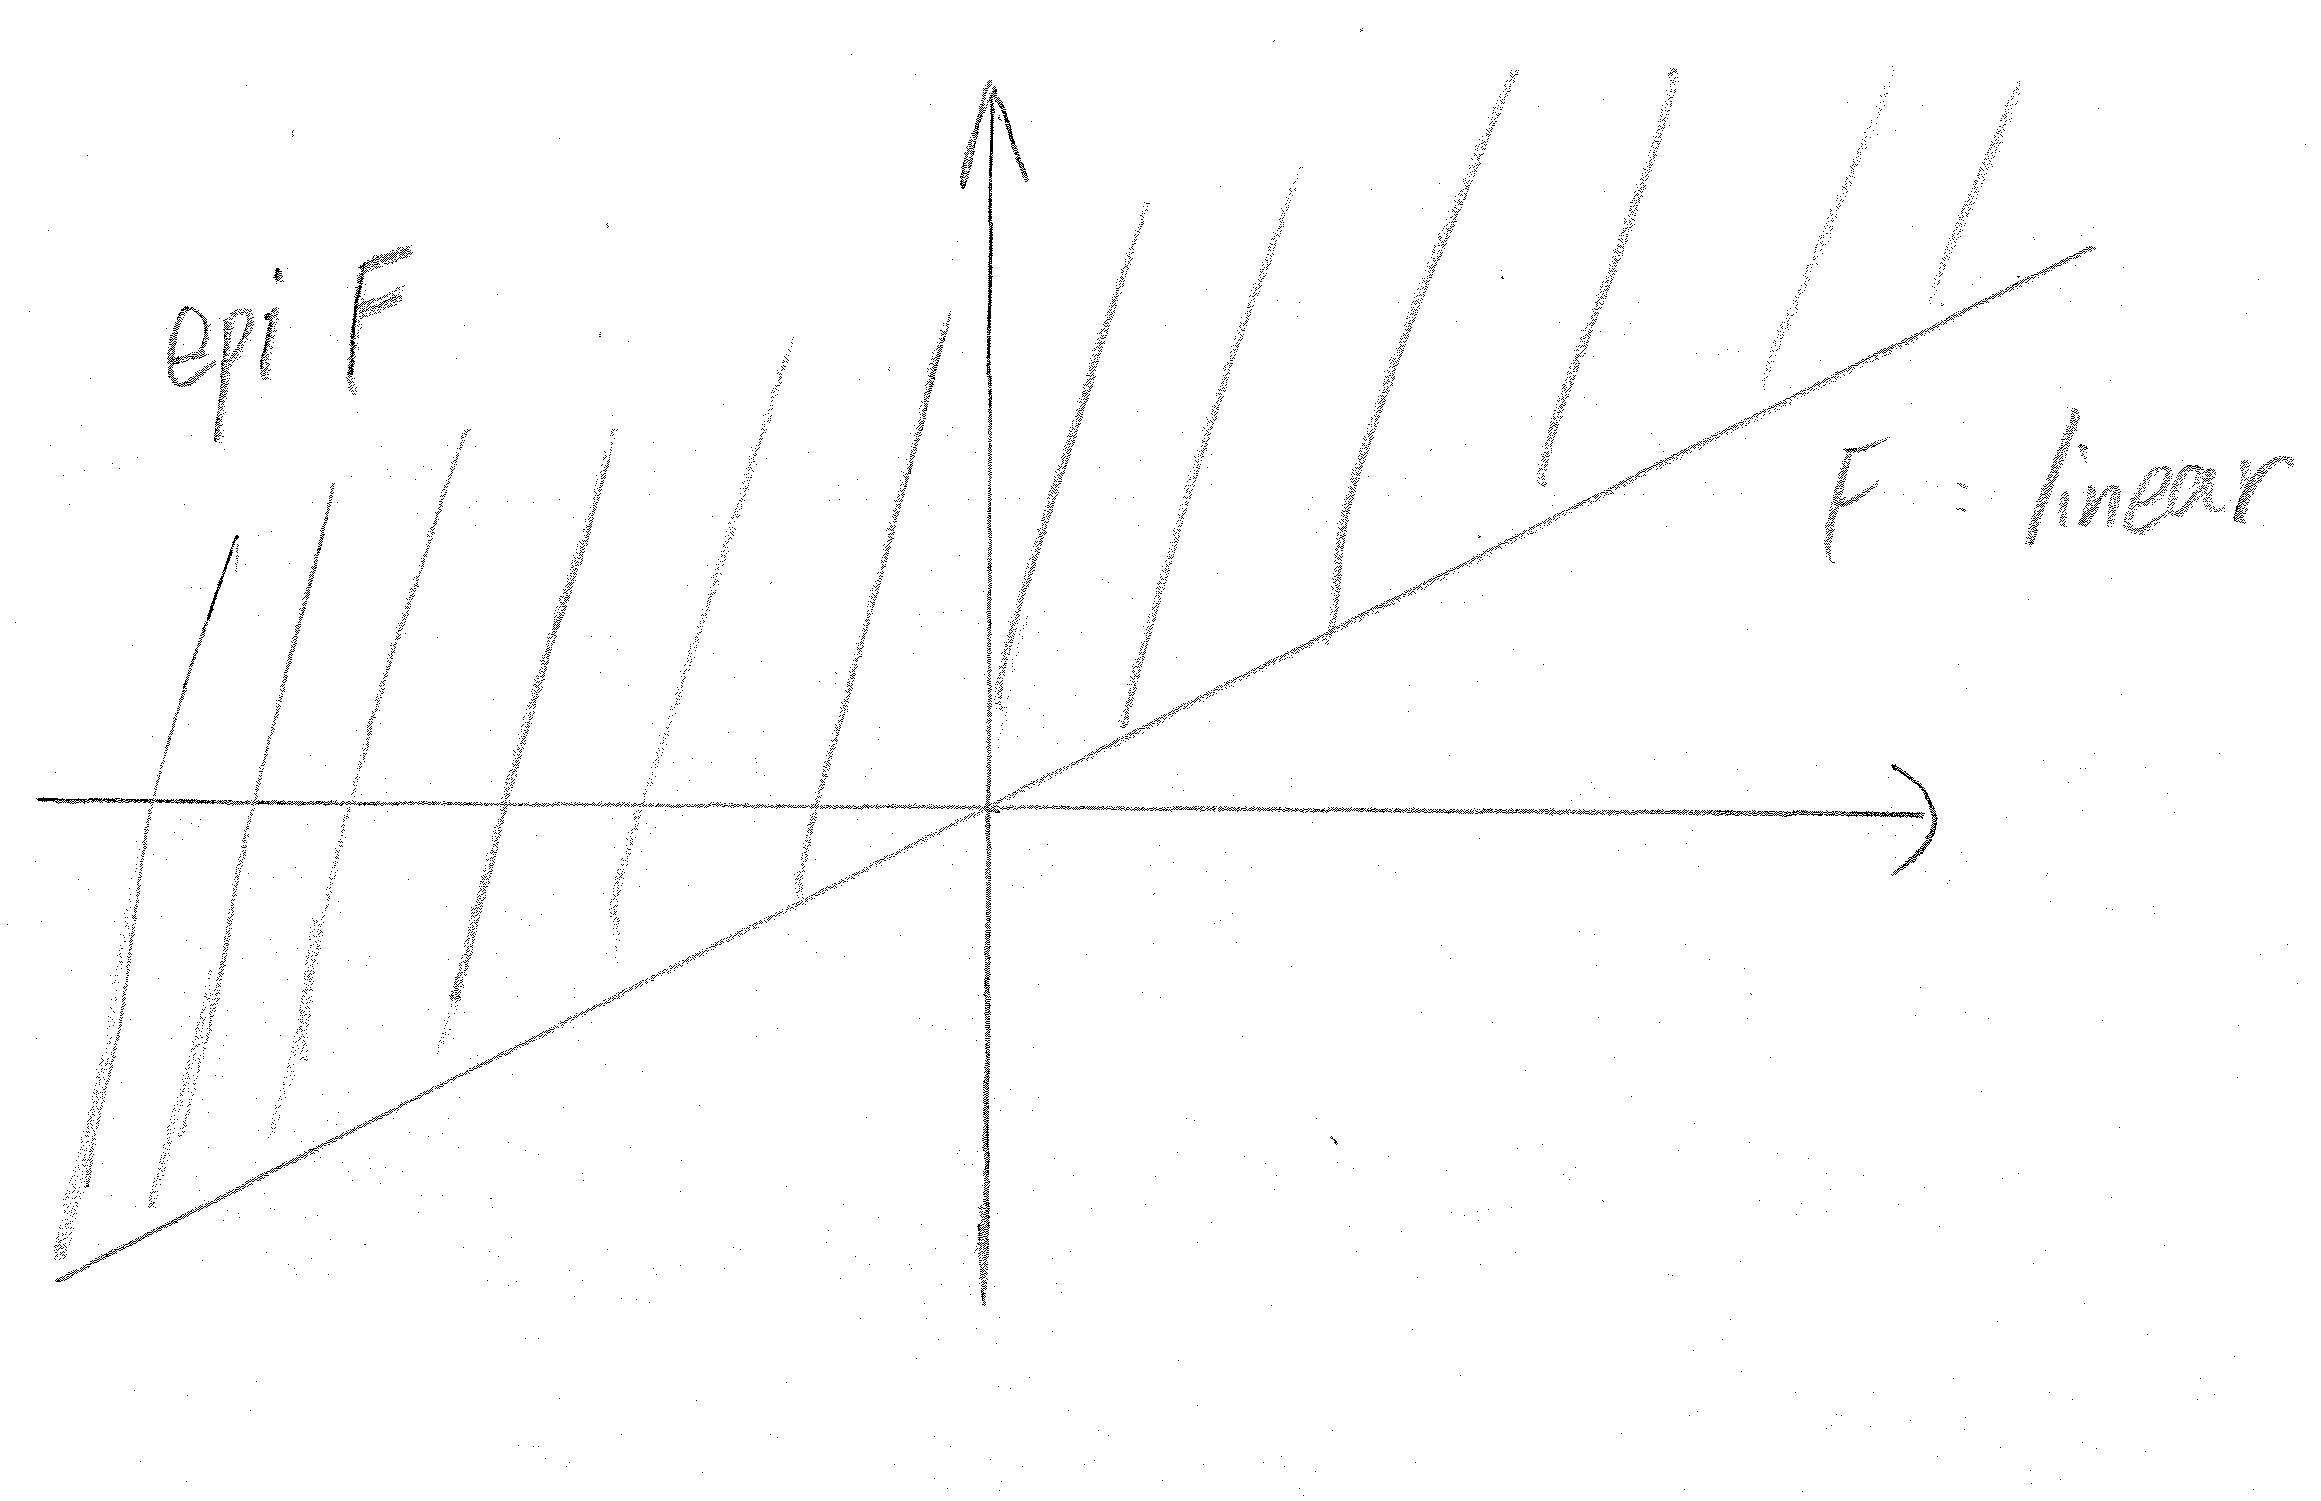
\includegraphics[width=2in,height=2in]{figures/ch02/p50-1.jpg}
	%\caption{This is an inserted JPG graphic} 
	%\label{fig:graph} 
\end{figure}

\begin{figure}
	\centering
	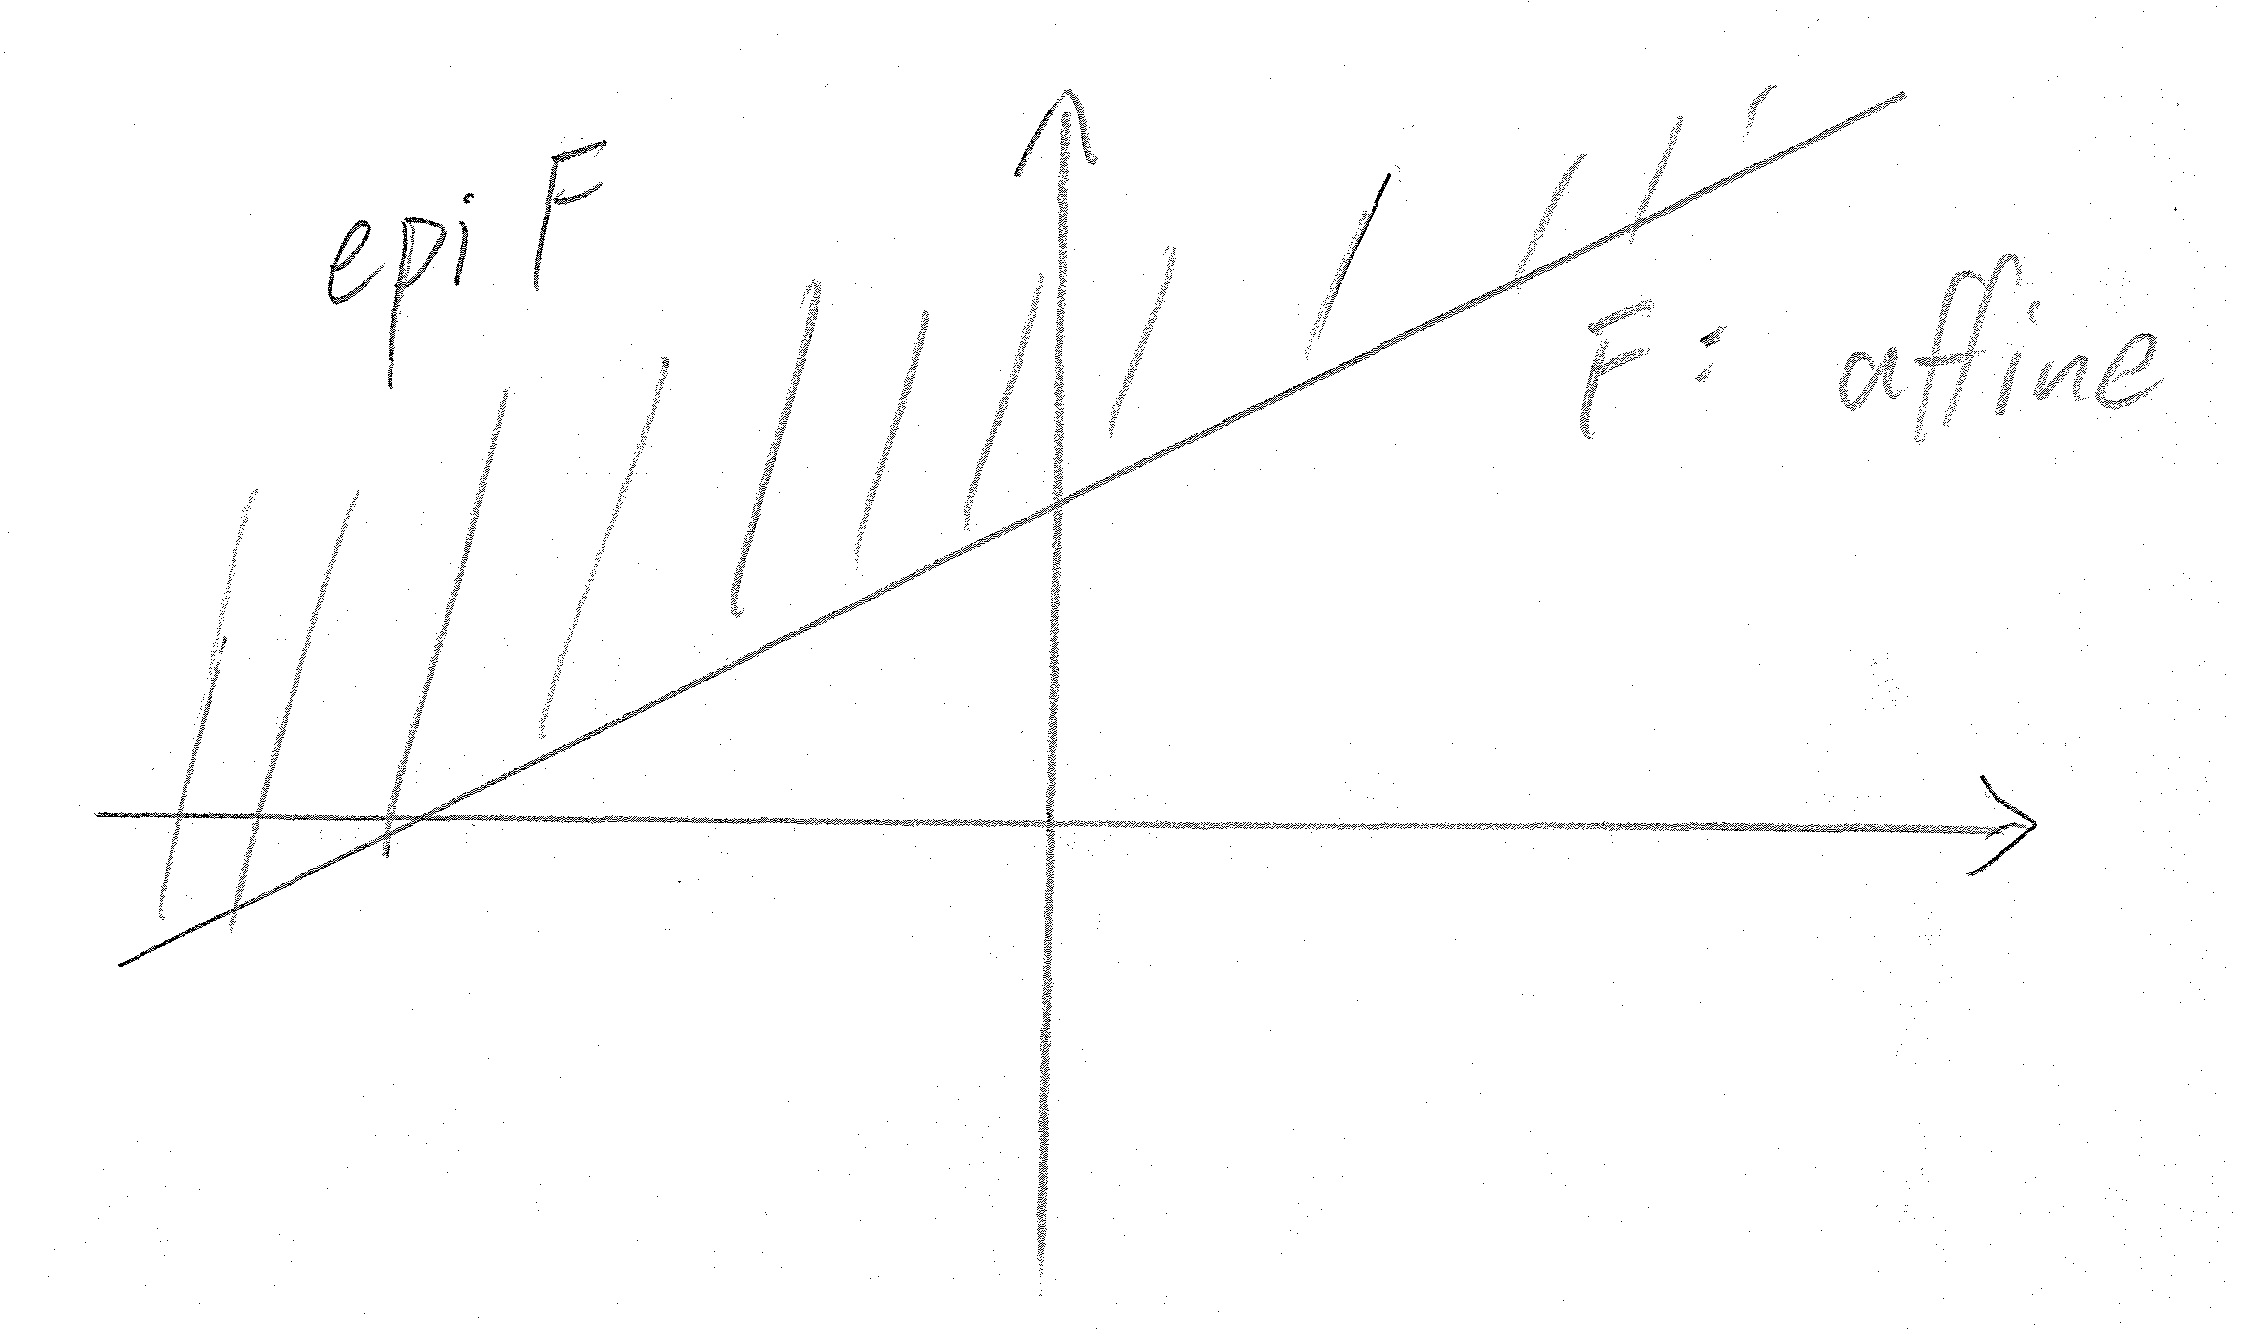
\includegraphics[width=2.1in,height=2.1in]{figures/ch02/p50-2.jpg}
	%\caption{This is an inserted JPG graphic} 
	%\label{fig:graph} 
\end{figure}


Similar statements hold for level sets and sub-level sets in $\reals^{n}$, e.g., level sets of a linear function $F:\reals^{2}\mapsto\reals$ are affine sets in $\reals^{2}$

\begin{figure}
	\centering
	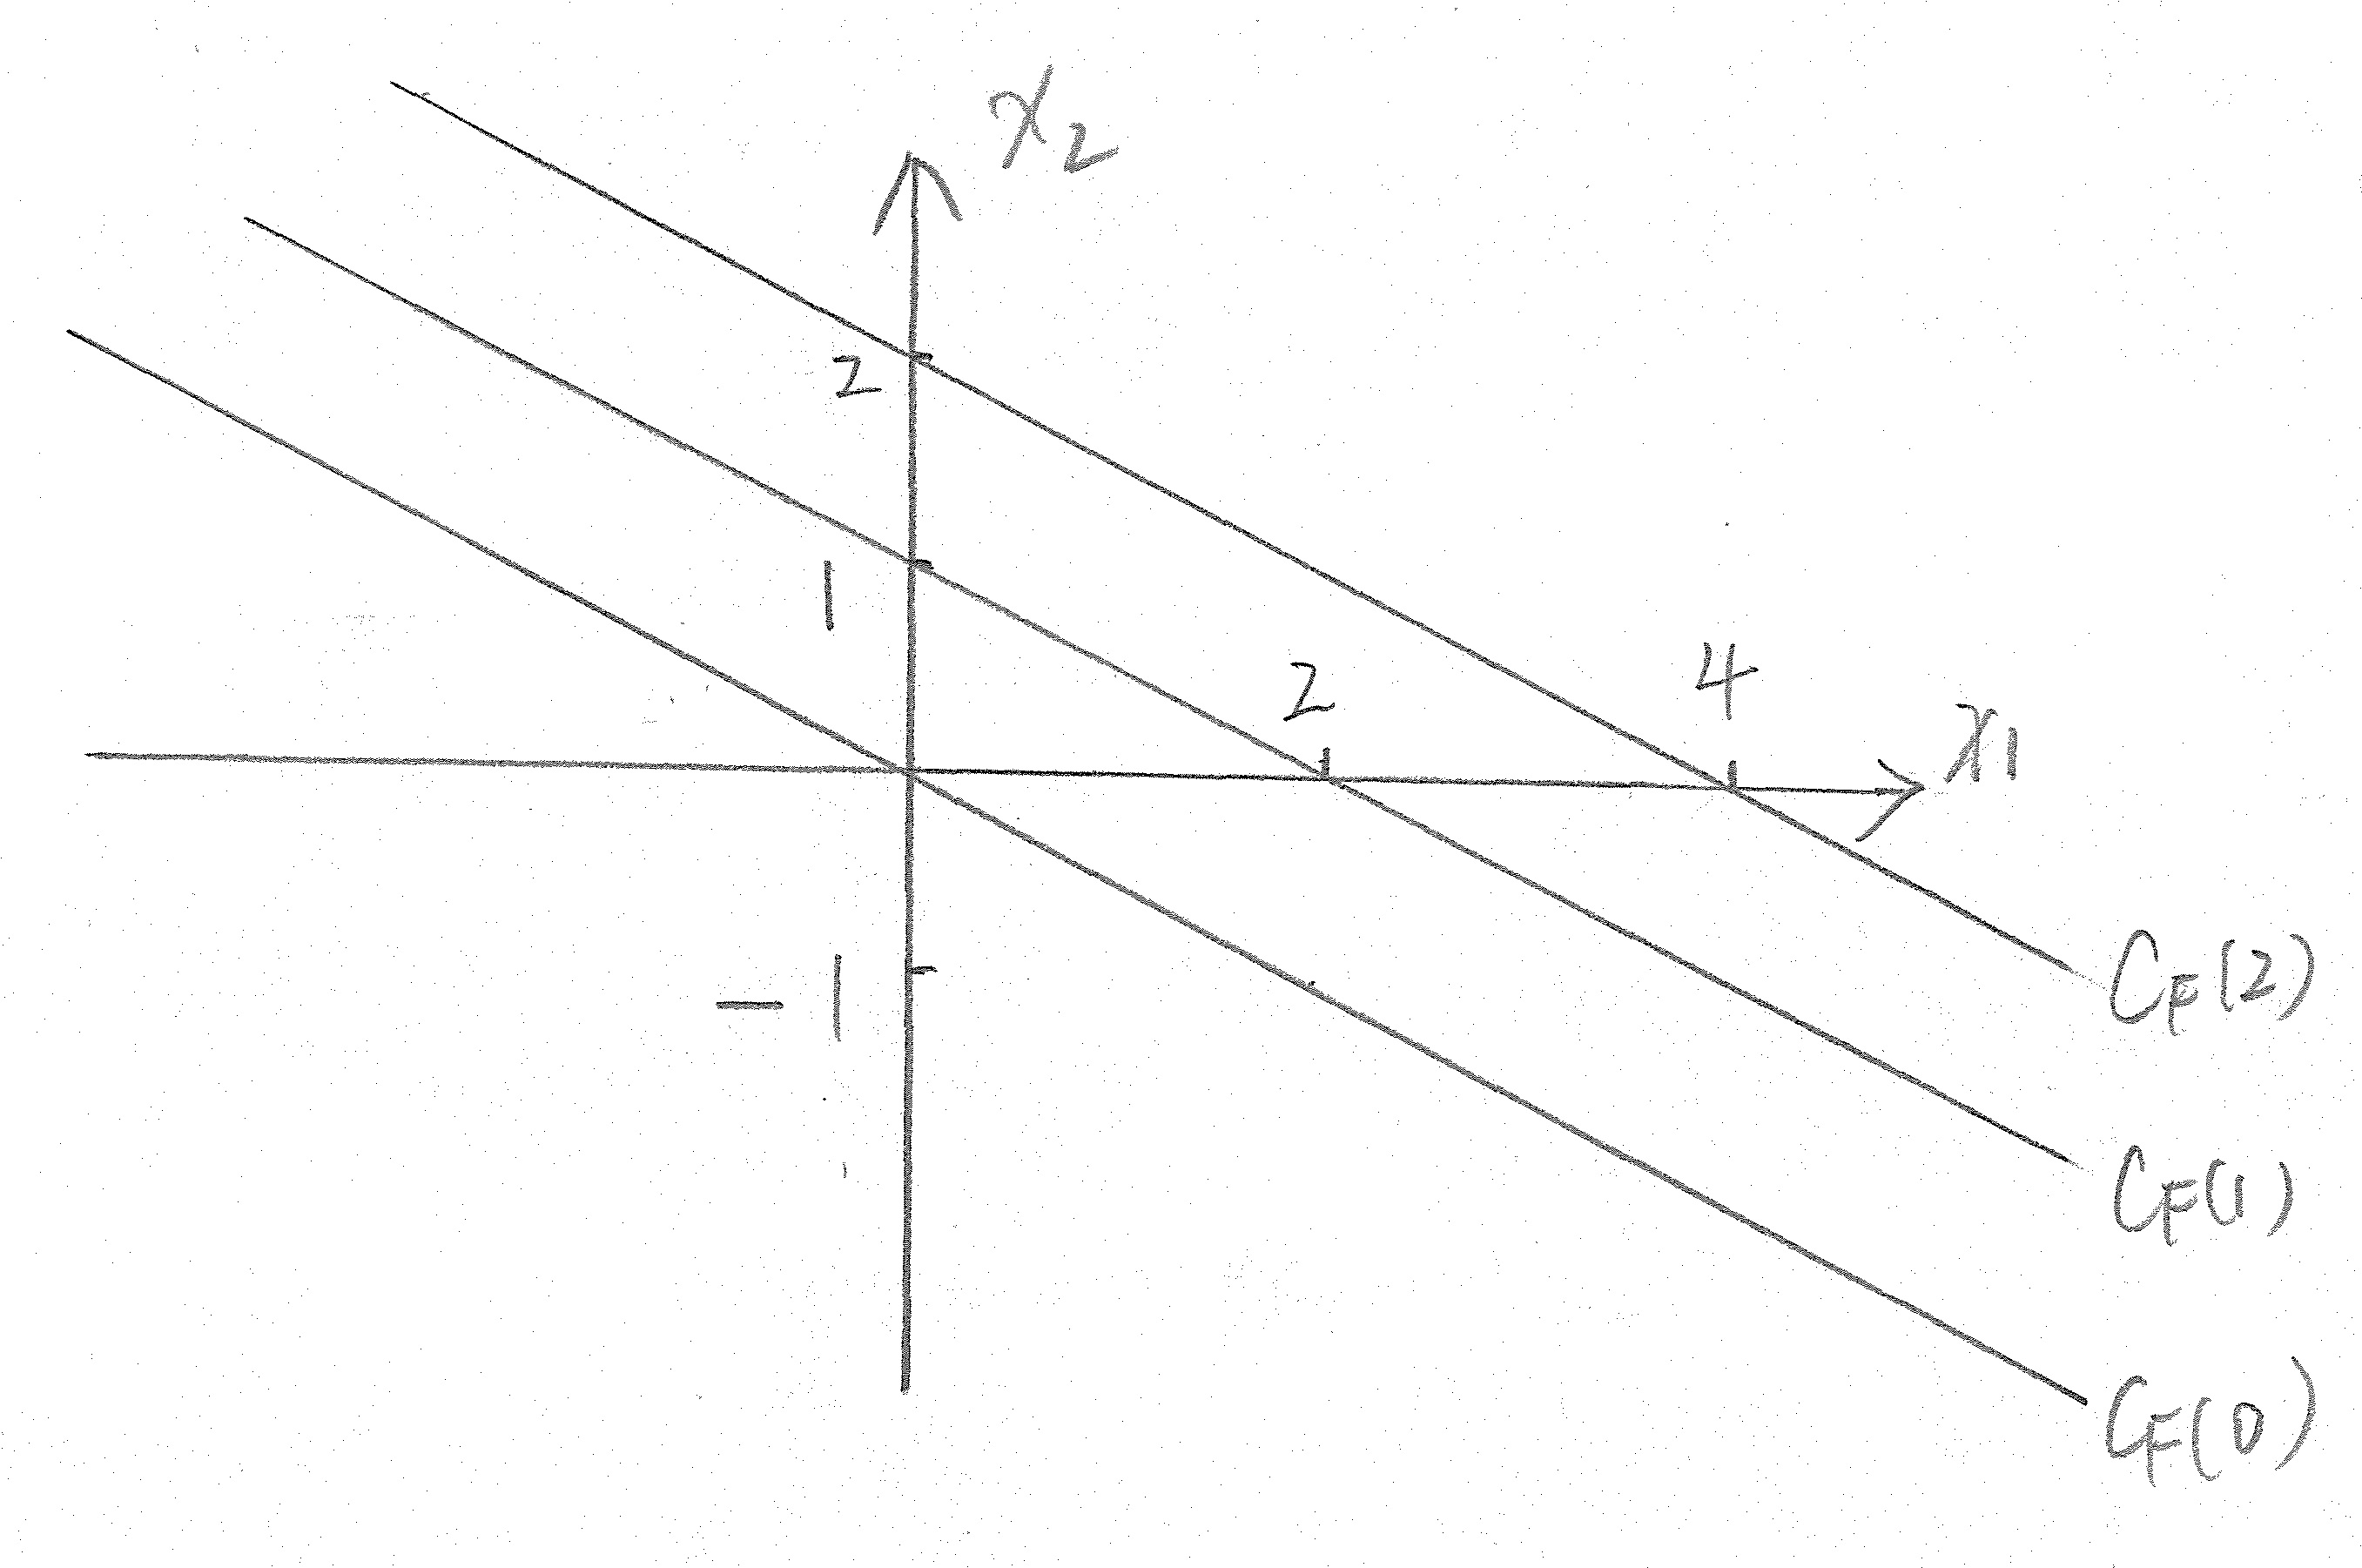
\includegraphics[width=2.1in,height=2.1in]{figures/ch02/p50-3.jpg}
	%\caption{This is an inserted JPG graphic} 
	%\label{fig:graph} 
\end{figure}

\vspace{0.3cm}
Definition of a hyperplane:
$$\mathcal{H}=\{z\in\reals^{n}|a^{\trans} z=b,a\in\reals^{n}, b\in\reals \}$$

\begin{marginfigure}
	\centering
	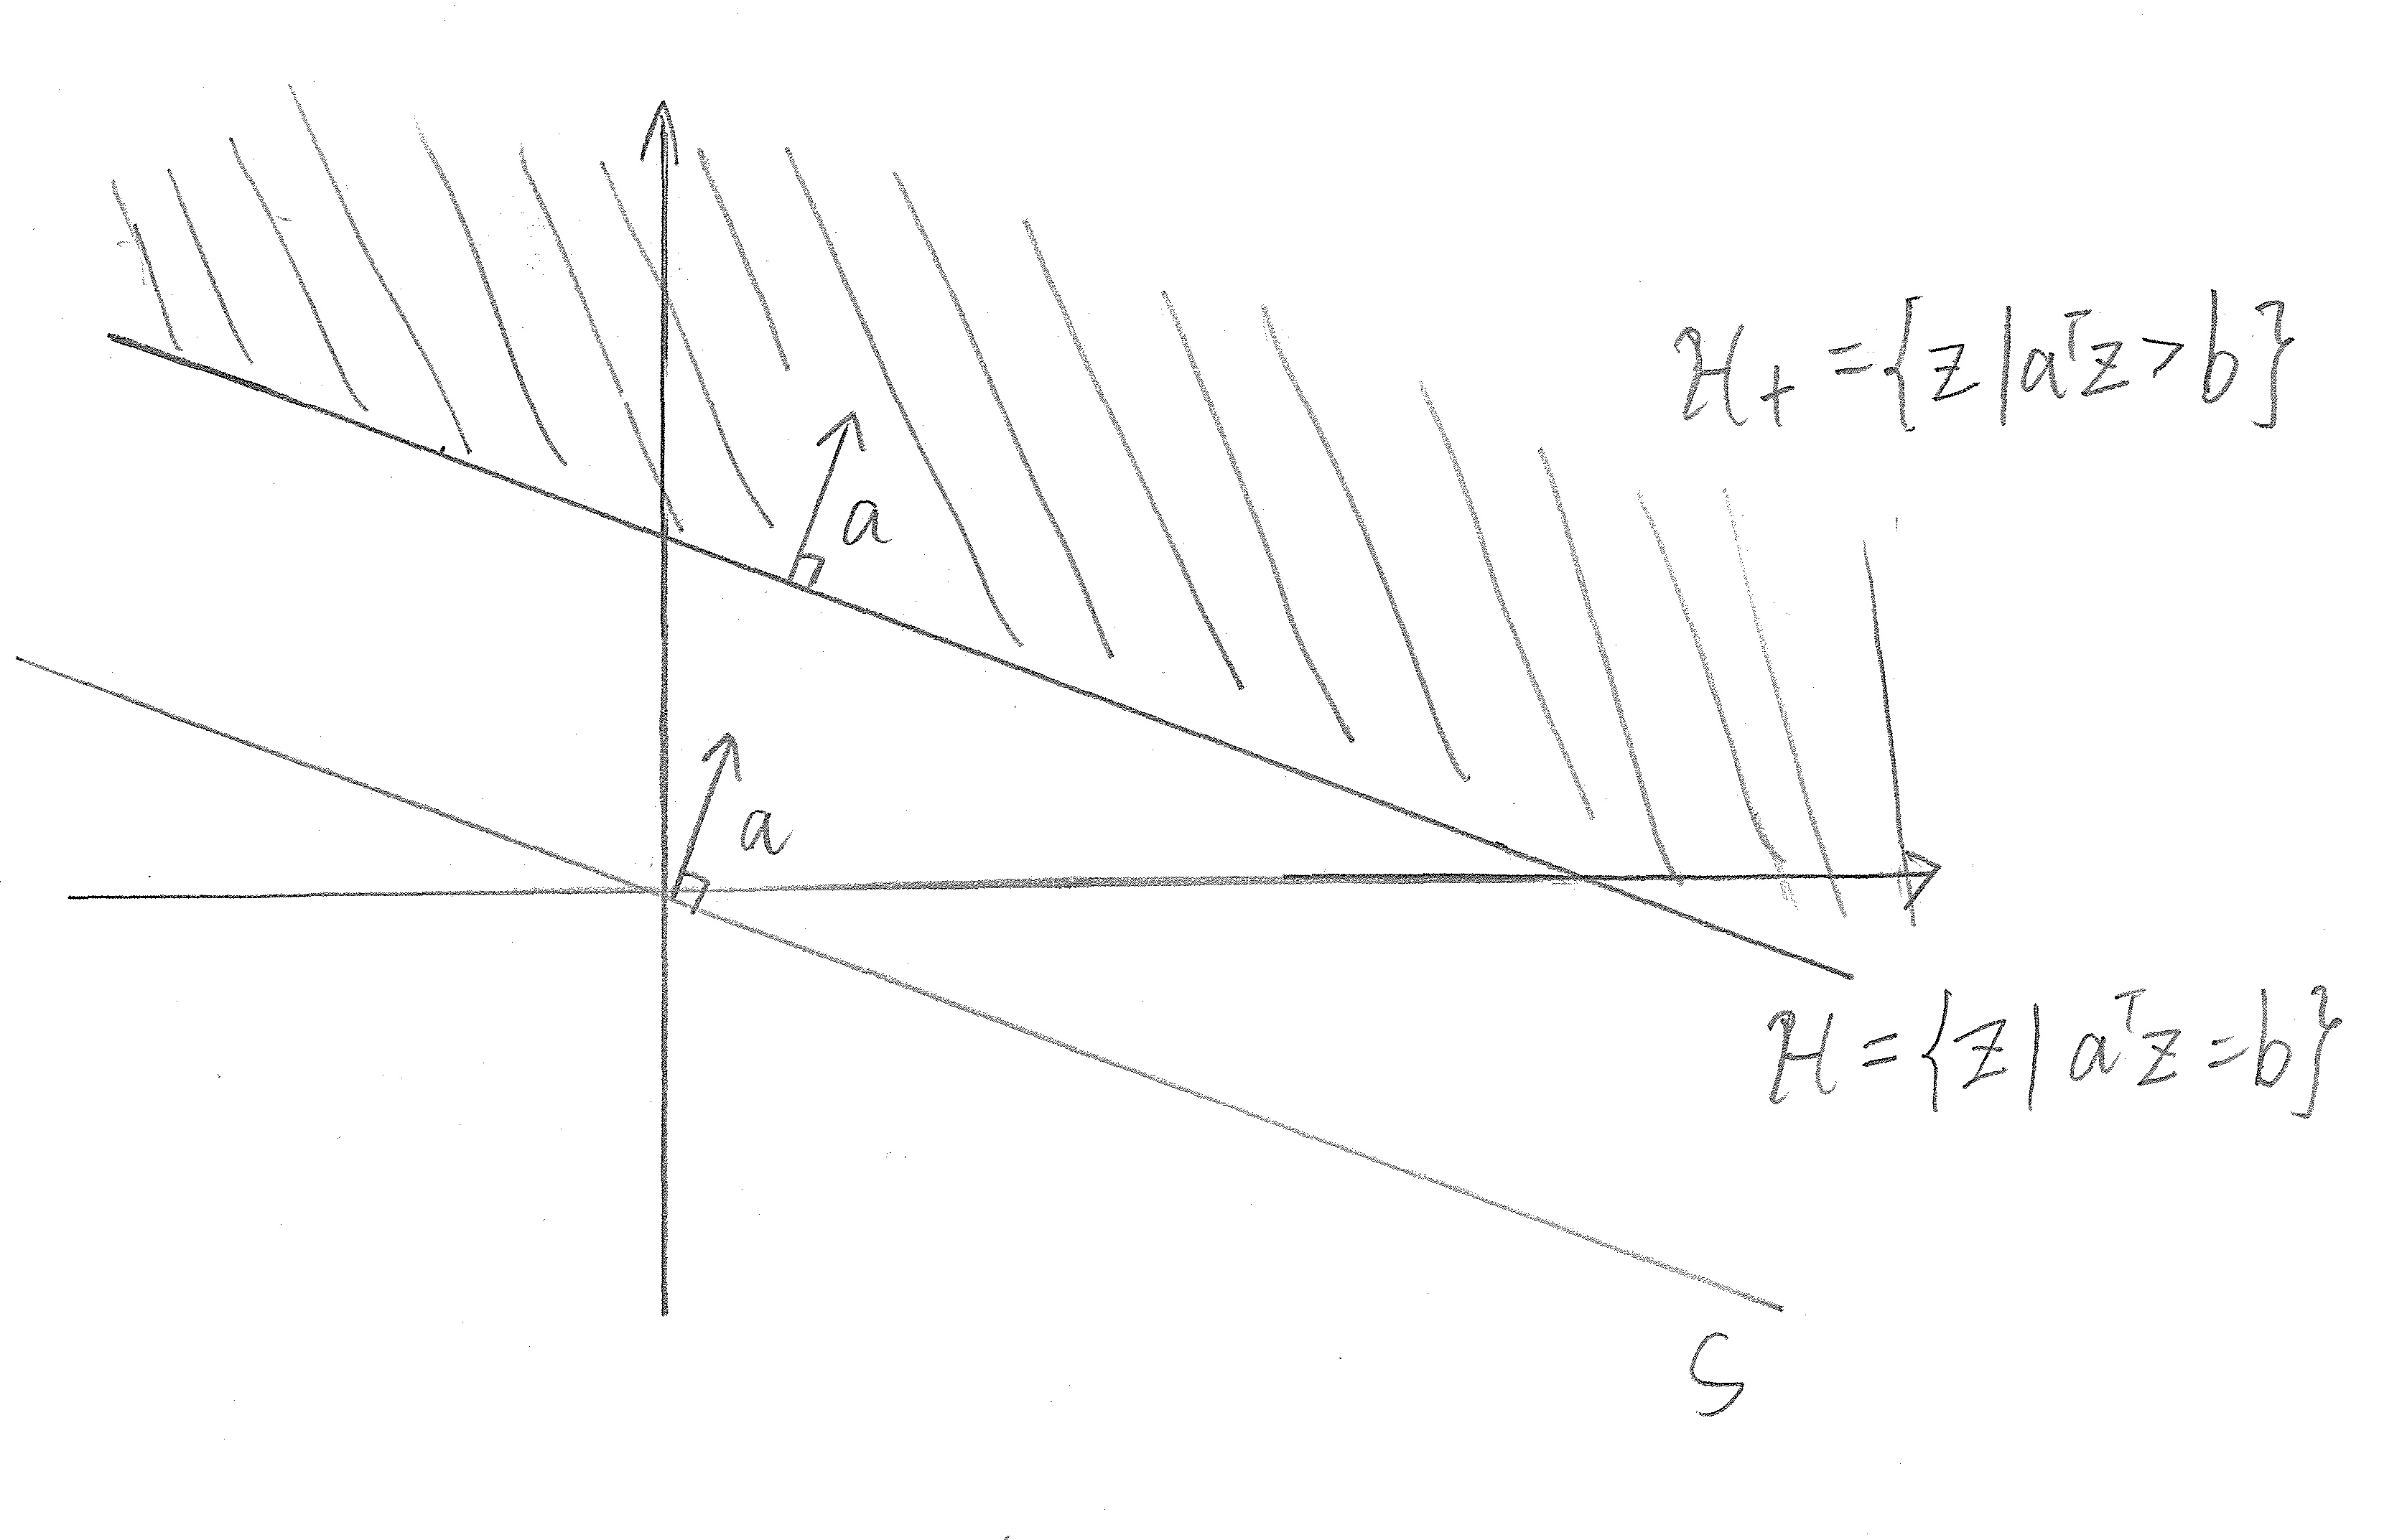
\includegraphics[width=2.1in,height=2.1in]{figures/ch02/p53.jpg}
	%\caption{This is an inserted JPG graphic} 
	\label{fig:graph} 
\end{marginfigure}

Definition of Half-spaces: are on one side or other of a hyperplane(see the r.h.s for a graph of $\mathcal{H}_{+}$),
$$\mathcal{H}_{+}=\{z\in\reals^{n}|a^{\trans} z>b\}$$
$$\mathcal{H}_{-}=\{z\in\reals^{n}|a^{\trans} z\leq b\}$$



\vspace{0.5cm}

\textbf{Gradient}

The gradient $\nabla F$ of $F:\reals^{n}\mapsto\reals$ is the vector of partial derivatives
$$\nabla F= 
\left[ 
\begin{array}{c} 
\frac{\partial F(x)}{\partial x_{1}} \\
\frac{\partial F(x)}{\partial x_{2}} \\
\vdots \\
\frac{\partial F(x)}{\partial x_{n}}
\end{array}
\right],
\ \text{where}\ x= 
\left[ 
\begin{array}{c} 
x_{1} \\
x_{2} \\
\vdots \\
x_{n}
\end{array}
\right]$$

Sometime  we need to consider compound function, and thus we need chain rule for gradients. Says, $g:\reals^{n}\mapsto\reals^{m}$ and $F:\reals^{m}\mapsto\reals$, both $F$ and $g$ are differentiable and we want $\nabla\Phi (x)$, where $\Phi (x)=F(g(x))$. In this case we have
$$
\nabla \phi (x)
=
\left[\begin{matrix}
	\frac{\partial \phi (x)}{\partial x_{1}}\\
	\vdots\\
	\vdots\\
	\frac{\partial \phi (x)}{\partial x_{n}}\\
\end{matrix}\right]
=
\left[\begin{matrix}
	\frac{\partial g_{1}(x)}{\partial x_{1}}&\frac{\partial g_{2}(x)}{\partial x_{1}}&\cdots&\frac{\partial g_{m}(x)}{\partial x_{1}}\\
	\frac{\partial g_{1}(x)}{\partial x_{2}}&\ddots & &\vdots\\
	\vdots& &\ddots &\vdots \\
	\frac{\partial g_{1}(x)}{\partial x_{n}}&\cdots&\cdots&\frac{\partial g_{m}(x)}{\partial x_{n}}
\end{matrix}\right]
\nabla F\left(g(x)\right)
$$

Example 

Let $g:\reals^{4}\mapsto\reals^{3}$ and $F:\reals^{3}\mapsto\reals$, both $F$ and $g$ are differentiable and we want to find $\nabla\Phi (x)$. To simplify, we let the function $g$ and $F$ takes the form,

$g(x)=Ax+b$, where $A$ is an $3$ by $4$ matrix, $x$ is a $4$ dimensions vector,  and $b$ is $3$ dimensions vector, so function $g$ maps $\reals^{4}$ to $\reals^{3}$.
 

$F(x)=Cx$, where $C$ is an $1$ by $3$ matrix and the input $x$ is a $3$ dimensions vector, so function $F$ maps $\reals^{3}$ to $\reals$.

Hence, the gradient of $\Phi (x)$ is
\begin{align*}
\nabla \phi (x) &=
\left[\begin{matrix}
\frac{\partial \phi (x)}{\partial x_{1}}\\
\frac{\partial \phi (x)}{\partial x_{2}}\\
\frac{\partial \phi (x)}{\partial x_{13}}\\
\frac{\partial \phi (x)}{\partial x_{4}}\\
\end{matrix}\right]\\
&=
\left[\begin{matrix}
\frac{\partial g_{1}(x)}{\partial x_{1}}&\frac{\partial g_{2}(x)}{\partial x_{1}}&\frac{\partial g_{3}(x)}{\partial x_{1}}\\
\frac{\partial g_{1}(x)}{\partial x_{2}}&\frac{\partial g_{2}(x)}{\partial x_{2}}&\frac{\partial g_{3}(x)}{\partial x_{2}}\\
\frac{\partial g_{1}(x)}{\partial x_{3}}&\frac{\partial g_{2}(x)}{\partial x_{3}}&\frac{\partial g_{3}(x)}{\partial x_{3}}\\
\frac{\partial g_{1}(x)}{\partial x_{4}}&\frac{\partial g_{2}(x)}{\partial x_{4}}&\frac{\partial g_{3}(x)}{\partial x_{4}}
\end{matrix}\right]
\left[\begin{matrix}
\frac{\partial \phi (x)}{\partial g_{1}}\\
\frac{\partial \phi (x)}{\partial g_{2}}\\
\frac{\partial \phi (x)}{\partial g_{3}}\\
\end{matrix}\right]\\
&=
\left[\begin{matrix}
a_{11}&a_{21}&a_{31}\\
a_{12}&a_{22}&a_{32}\\
a_{13}&a_{23}&a_{33}\\
a_{14}&a_{24}&a_{34}\\
\end{matrix}\right]
\left[\begin{matrix}
c_{11}\\
c_{12}\\
c_{13}\\
\end{matrix}\right]\\
&=
A^{\trans}C^{\trans}\\
\end{align*}

\textbf{Affine approximations}

Consider the Taylor series for $F\colon \mathbb{R}^n \to \mathbb{R}$.

$$F(x) = F(x_0) + \nabla F(x_0)^{T} (x - x_0) + \varepsilon (x) $$


Example 1. $F(x) = 2 x_1^2 + x_2^2$

$$F(x) \cong F(x^{(0)}) + \nabla F(x^{(0)})^{T} (x - x^{(0)})
\left. \nabla F(x) \right|_{x} \qquad (*)$$

$$\nabla F(x) = \begin{bmatrix} 4x_1\\ 2x_2\\ \end{bmatrix}$$

\begin{displaymath}
\nabla F \left( \begin{bmatrix} 0\\ 0\\ \end{bmatrix} \right)  =
\begin{bmatrix} 0\\ 0\\ \end{bmatrix}
\end{displaymath}

\begin{displaymath}
\nabla F \left( \begin{bmatrix} 1\\ 0\\ \end{bmatrix} \right)  =
\begin{bmatrix} 4\\ 0\\ \end{bmatrix}
\end{displaymath}

\begin{displaymath}
\nabla F \left( \begin{bmatrix} 0\\ 1\\ \end{bmatrix} \right)  =
\begin{bmatrix} 0\\ 2\\ \end{bmatrix}
\end{displaymath}


\begin{figure}
	\centering
	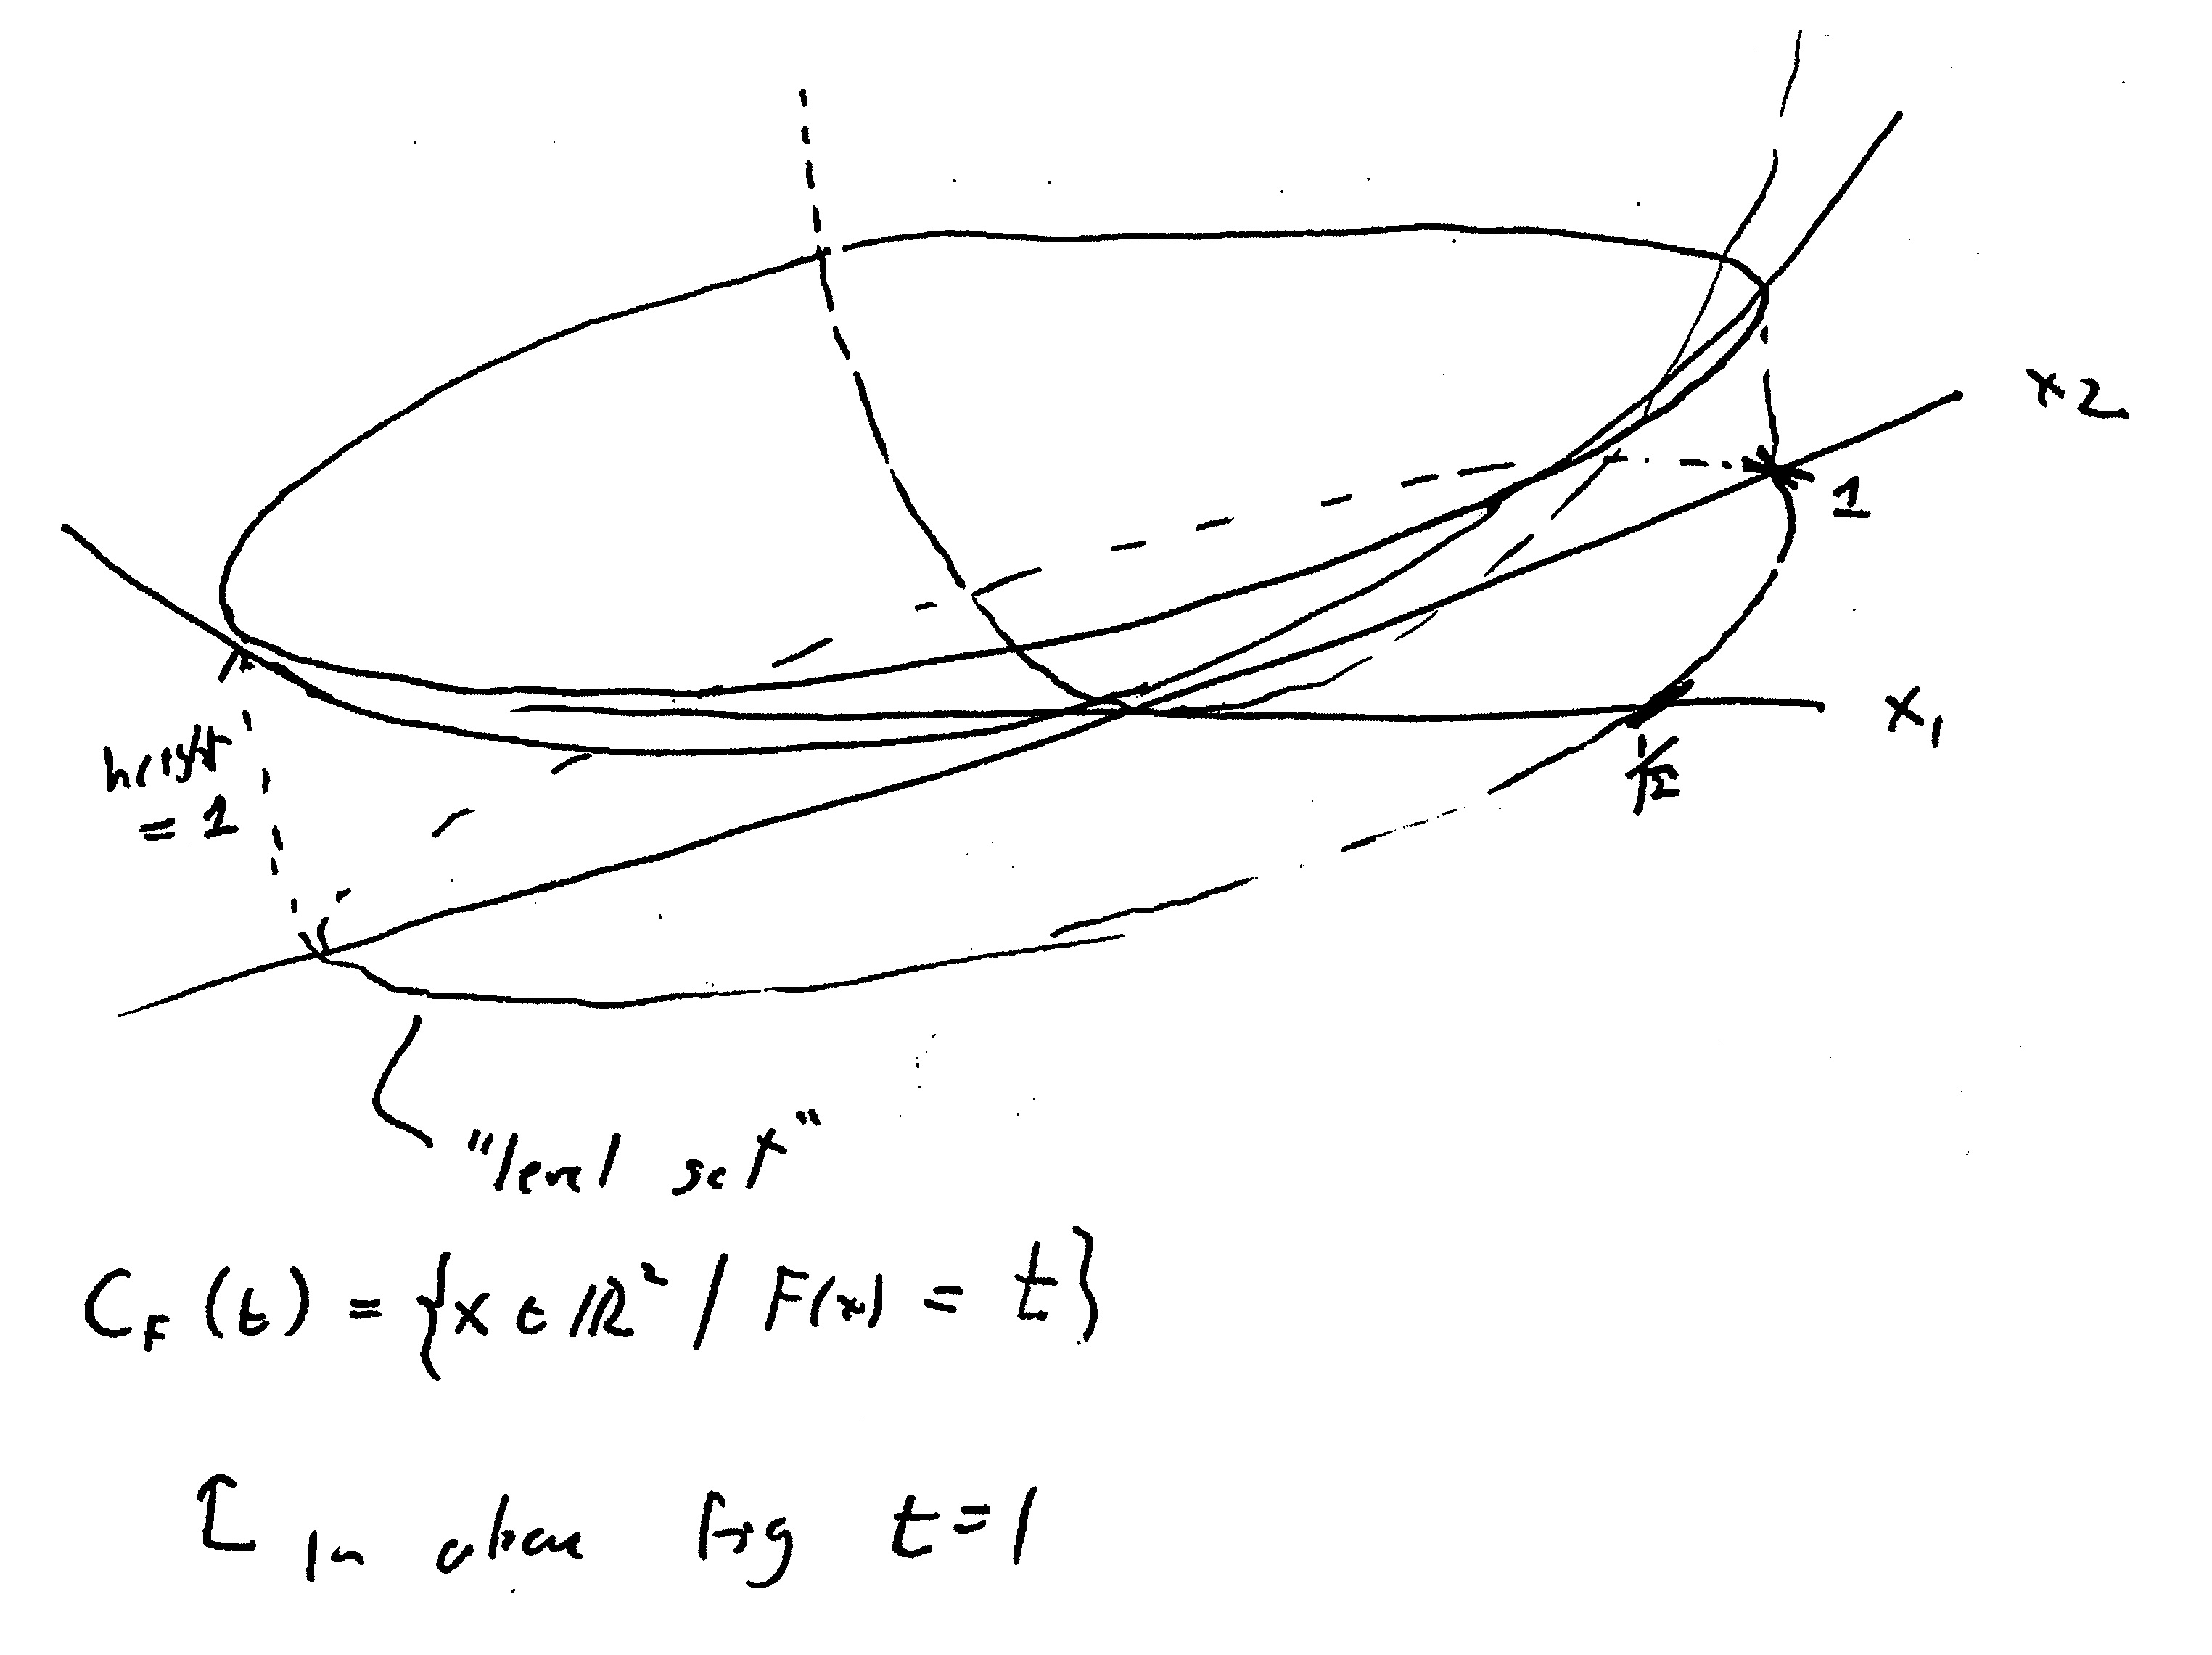
\includegraphics[width=3in,height=3in]{figures/ch02/p59.jpg}
	%\caption{This is an inserted JPG graphic} 
	%\label{fig:graph} 
\end{figure}

Let's sketch the "level set" in 2-D, 

\begin{figure}
	\centering
	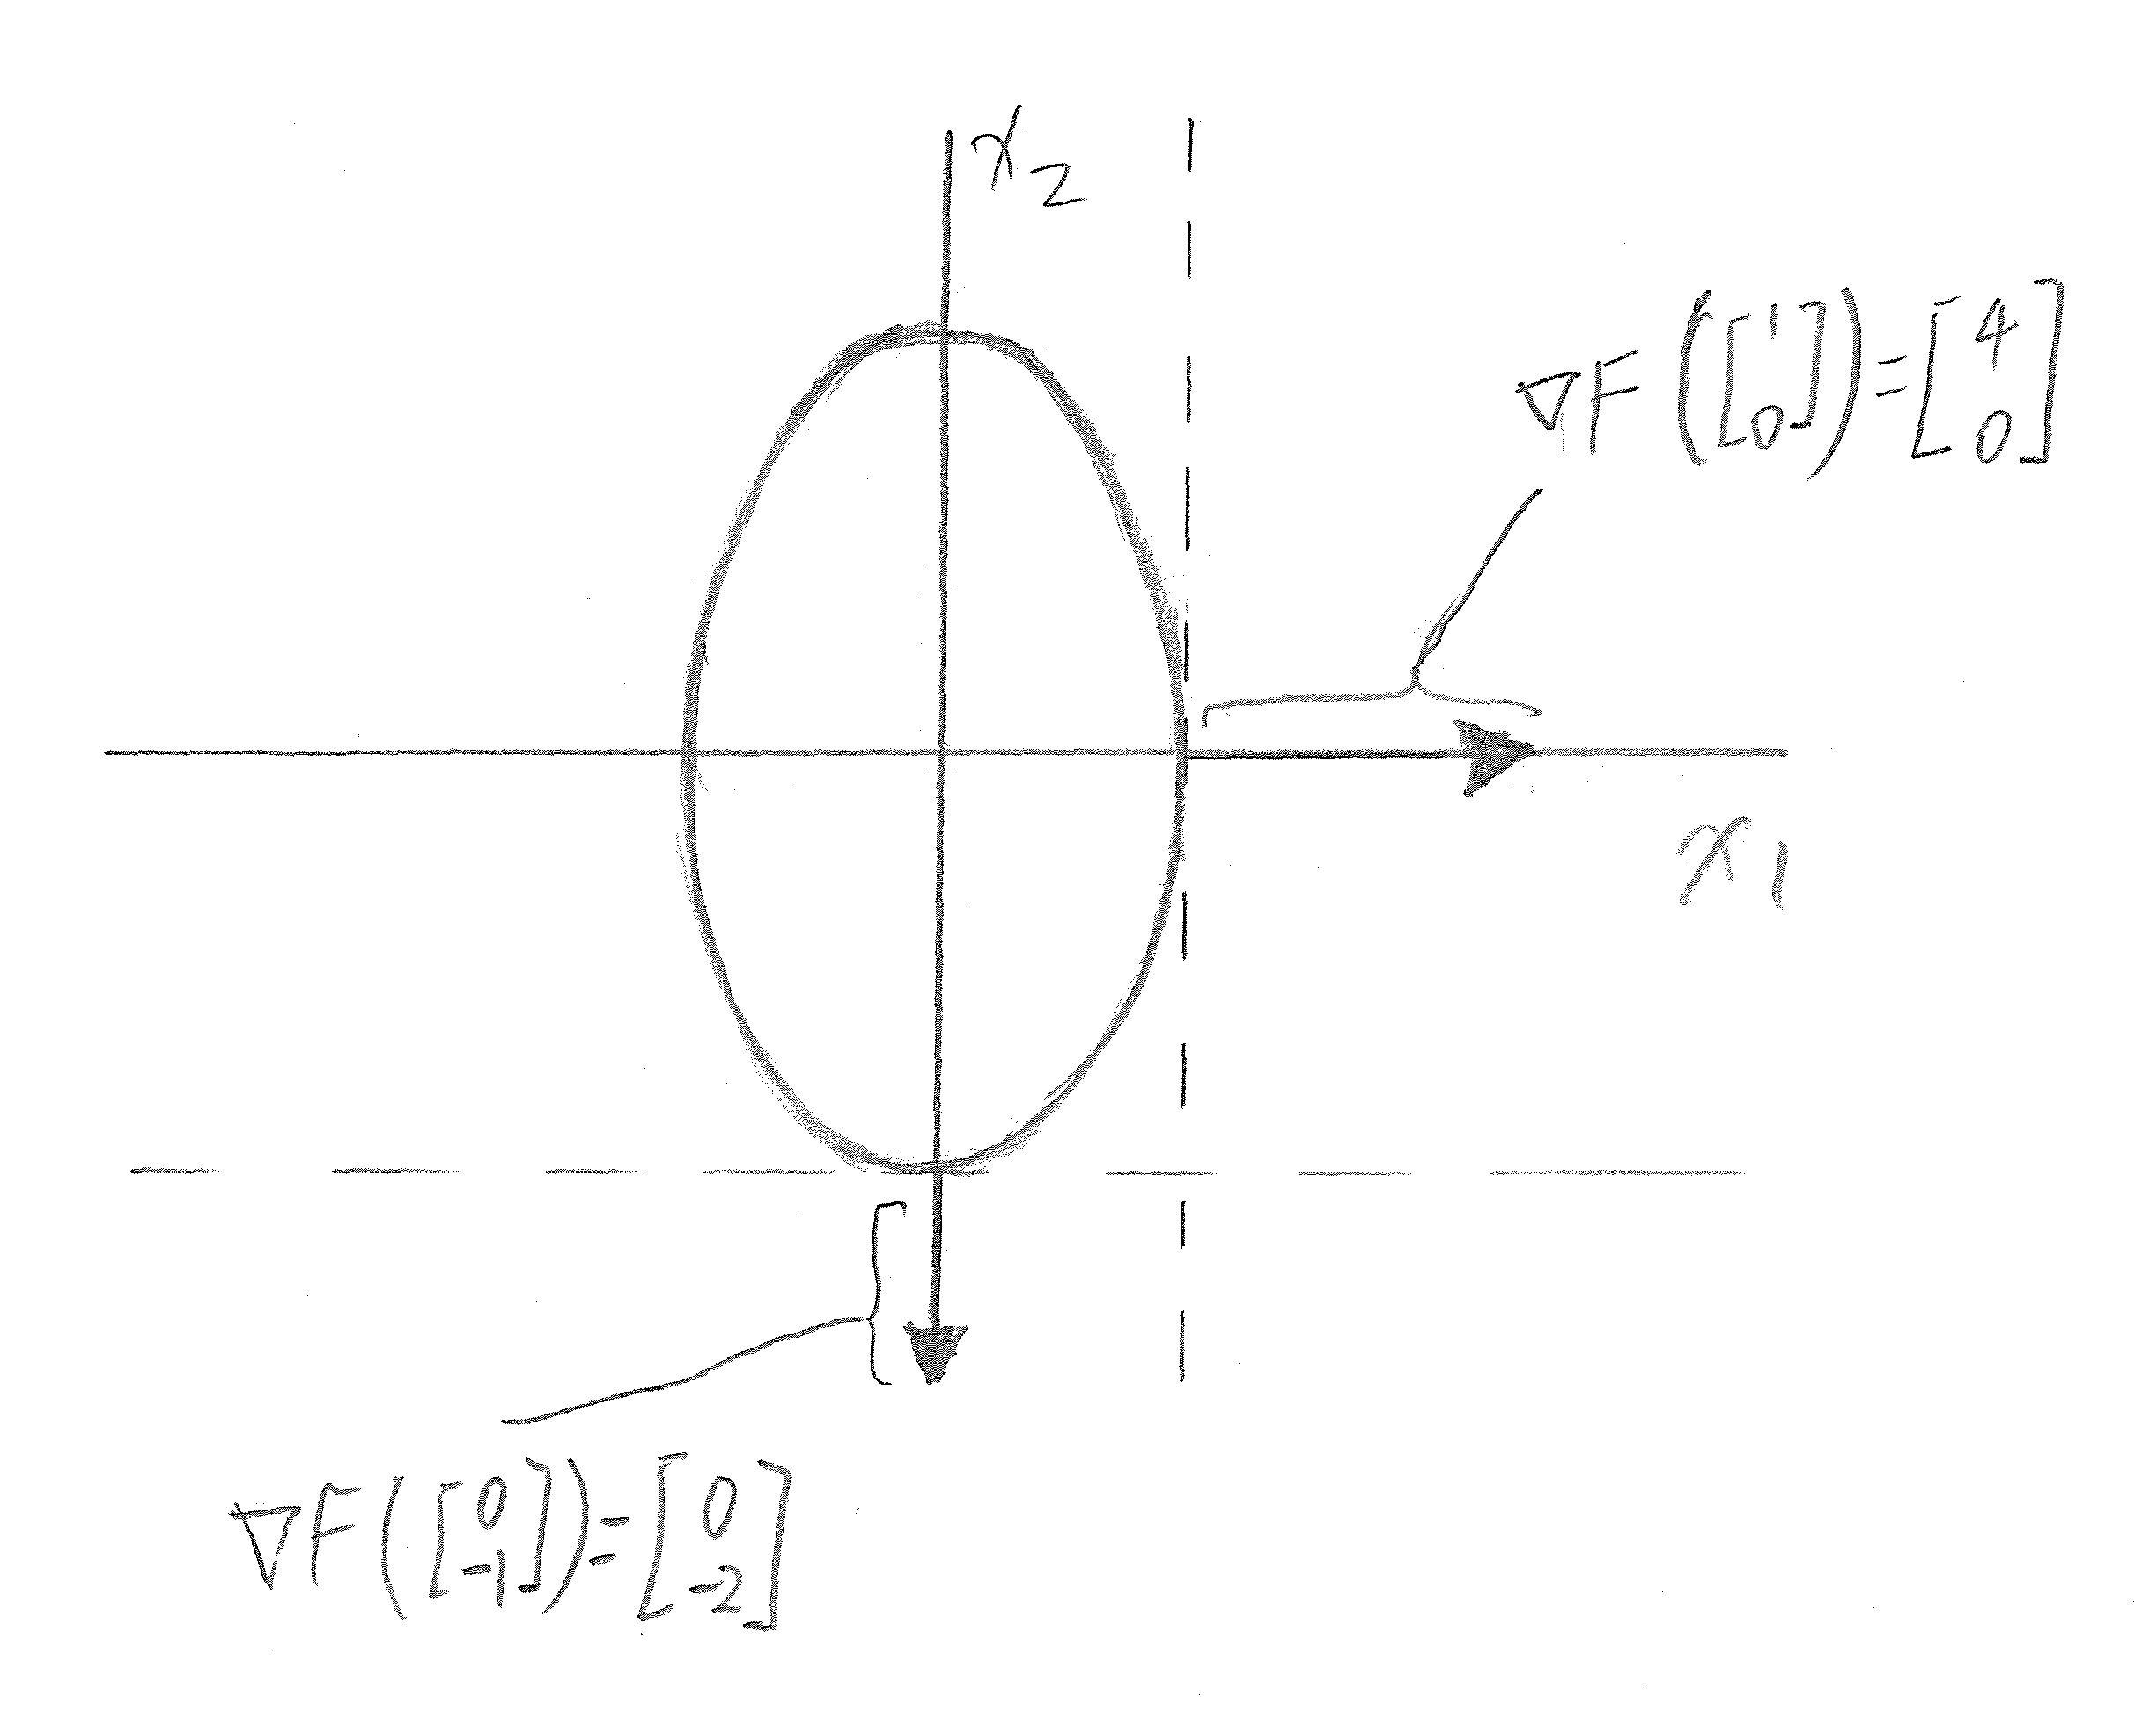
\includegraphics[width=2.1in,height=2.1in]{figures/ch02/p60-1.jpg}
	%\caption{This is an inserted JPG graphic} 
	%\label{fig:graph} 
\end{figure}

\begin{displaymath}
\nabla F \left( \begin{bmatrix} 1\\ 0\\ \end{bmatrix} \right)  =
\begin{bmatrix} 4\\ 0\\ \end{bmatrix}
\end{displaymath}

\begin{displaymath}
\nabla F \left( \begin{bmatrix} 0\\ -1\\ \end{bmatrix} \right)  =
\begin{bmatrix} 0\\ -2\\ \end{bmatrix}
\end{displaymath}

Let's visualize the set such that the increment in $(*)$ is, to first order, constant. That is, which $x \in \mathbb{R}^2$ satisfy the relation
$$\{x | \nabla F(x_0)^{T} (x-x_0) = c\}$$


(1) Consider case $c=0$

There are points s.t., to approximate $(*)$, has some level as $F(x_0)$ when $c=0$, we have the set $\{x | \nabla F(x_0)^{T} (x-x_0) = 0\}$

\begin{figure}
	\centering
	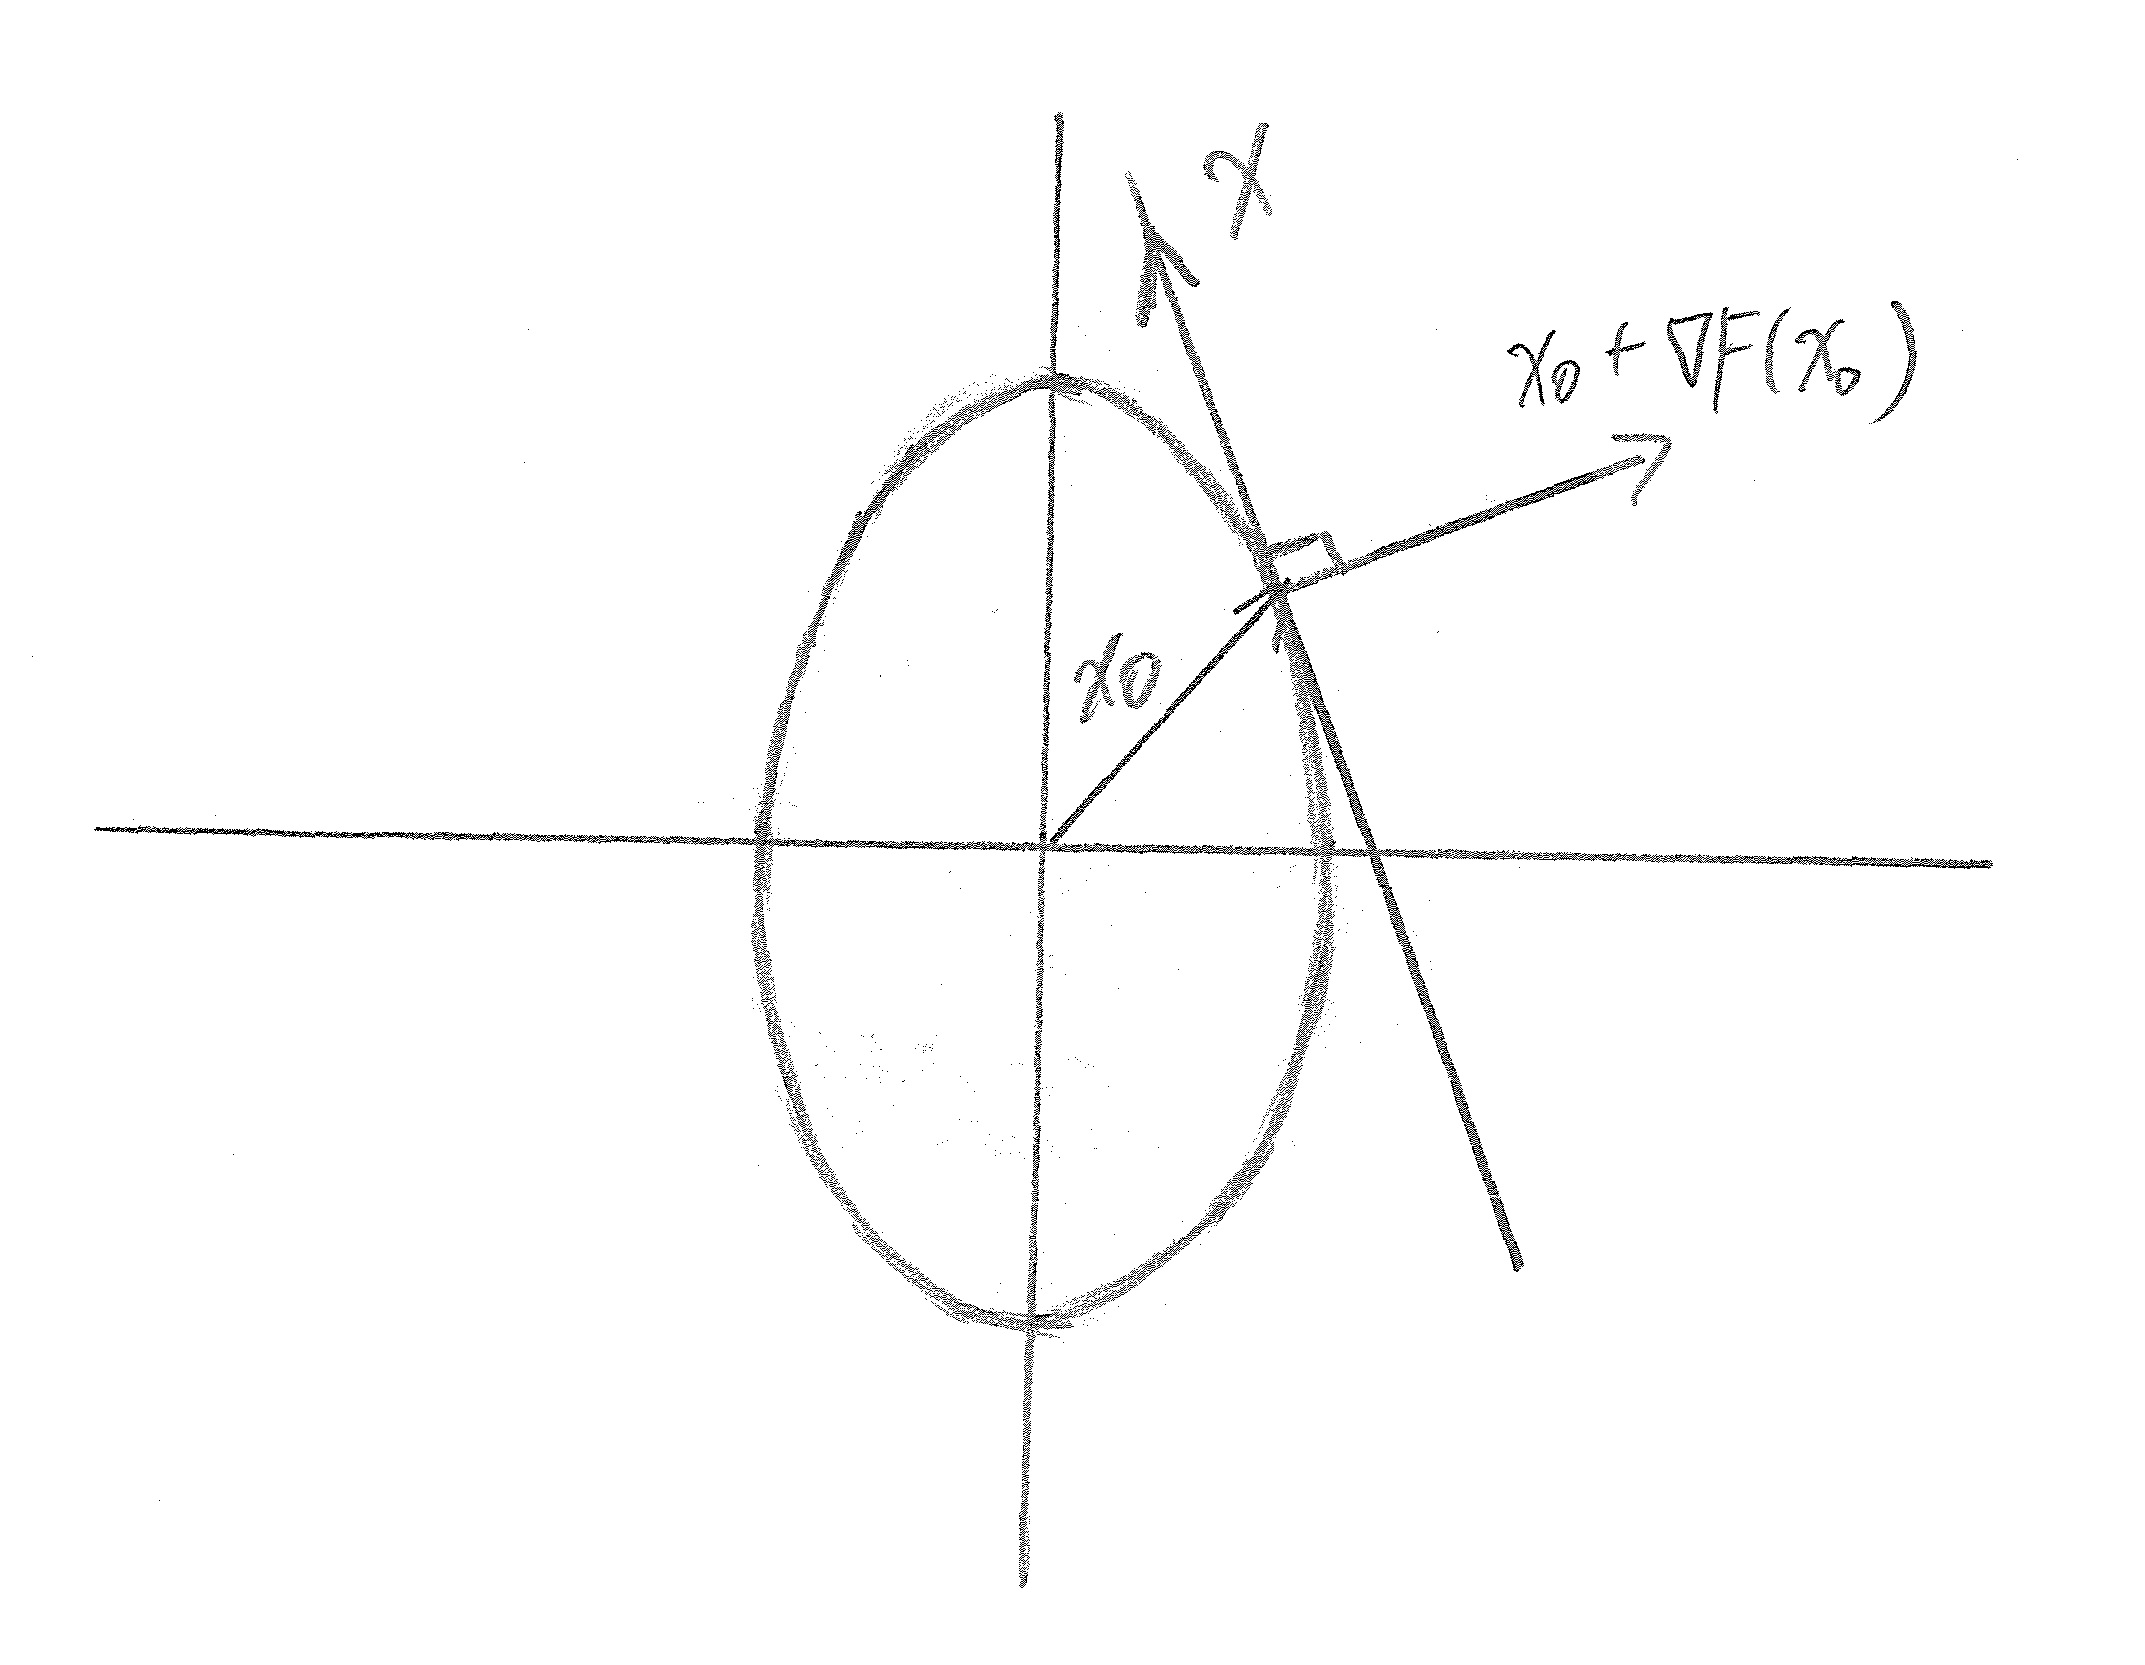
\includegraphics[width=2.1in,height=2.1in]{figures/ch02/p60-2.jpg}
	%\caption{This is an inserted JPG graphic} 
	%\label{fig:graph} 
\end{figure}


(2) Consider $c = \varepsilon > 0$, a small positive increment. Then, 
$$\{x | \nabla F(x_0)^{T} (x-x_0) = \varepsilon\}$$
is points that, to first order, have slightly higher cost (value, level). Then $F(x_0)$, the value at $x=x_0$.

\begin{figure}
	\centering
	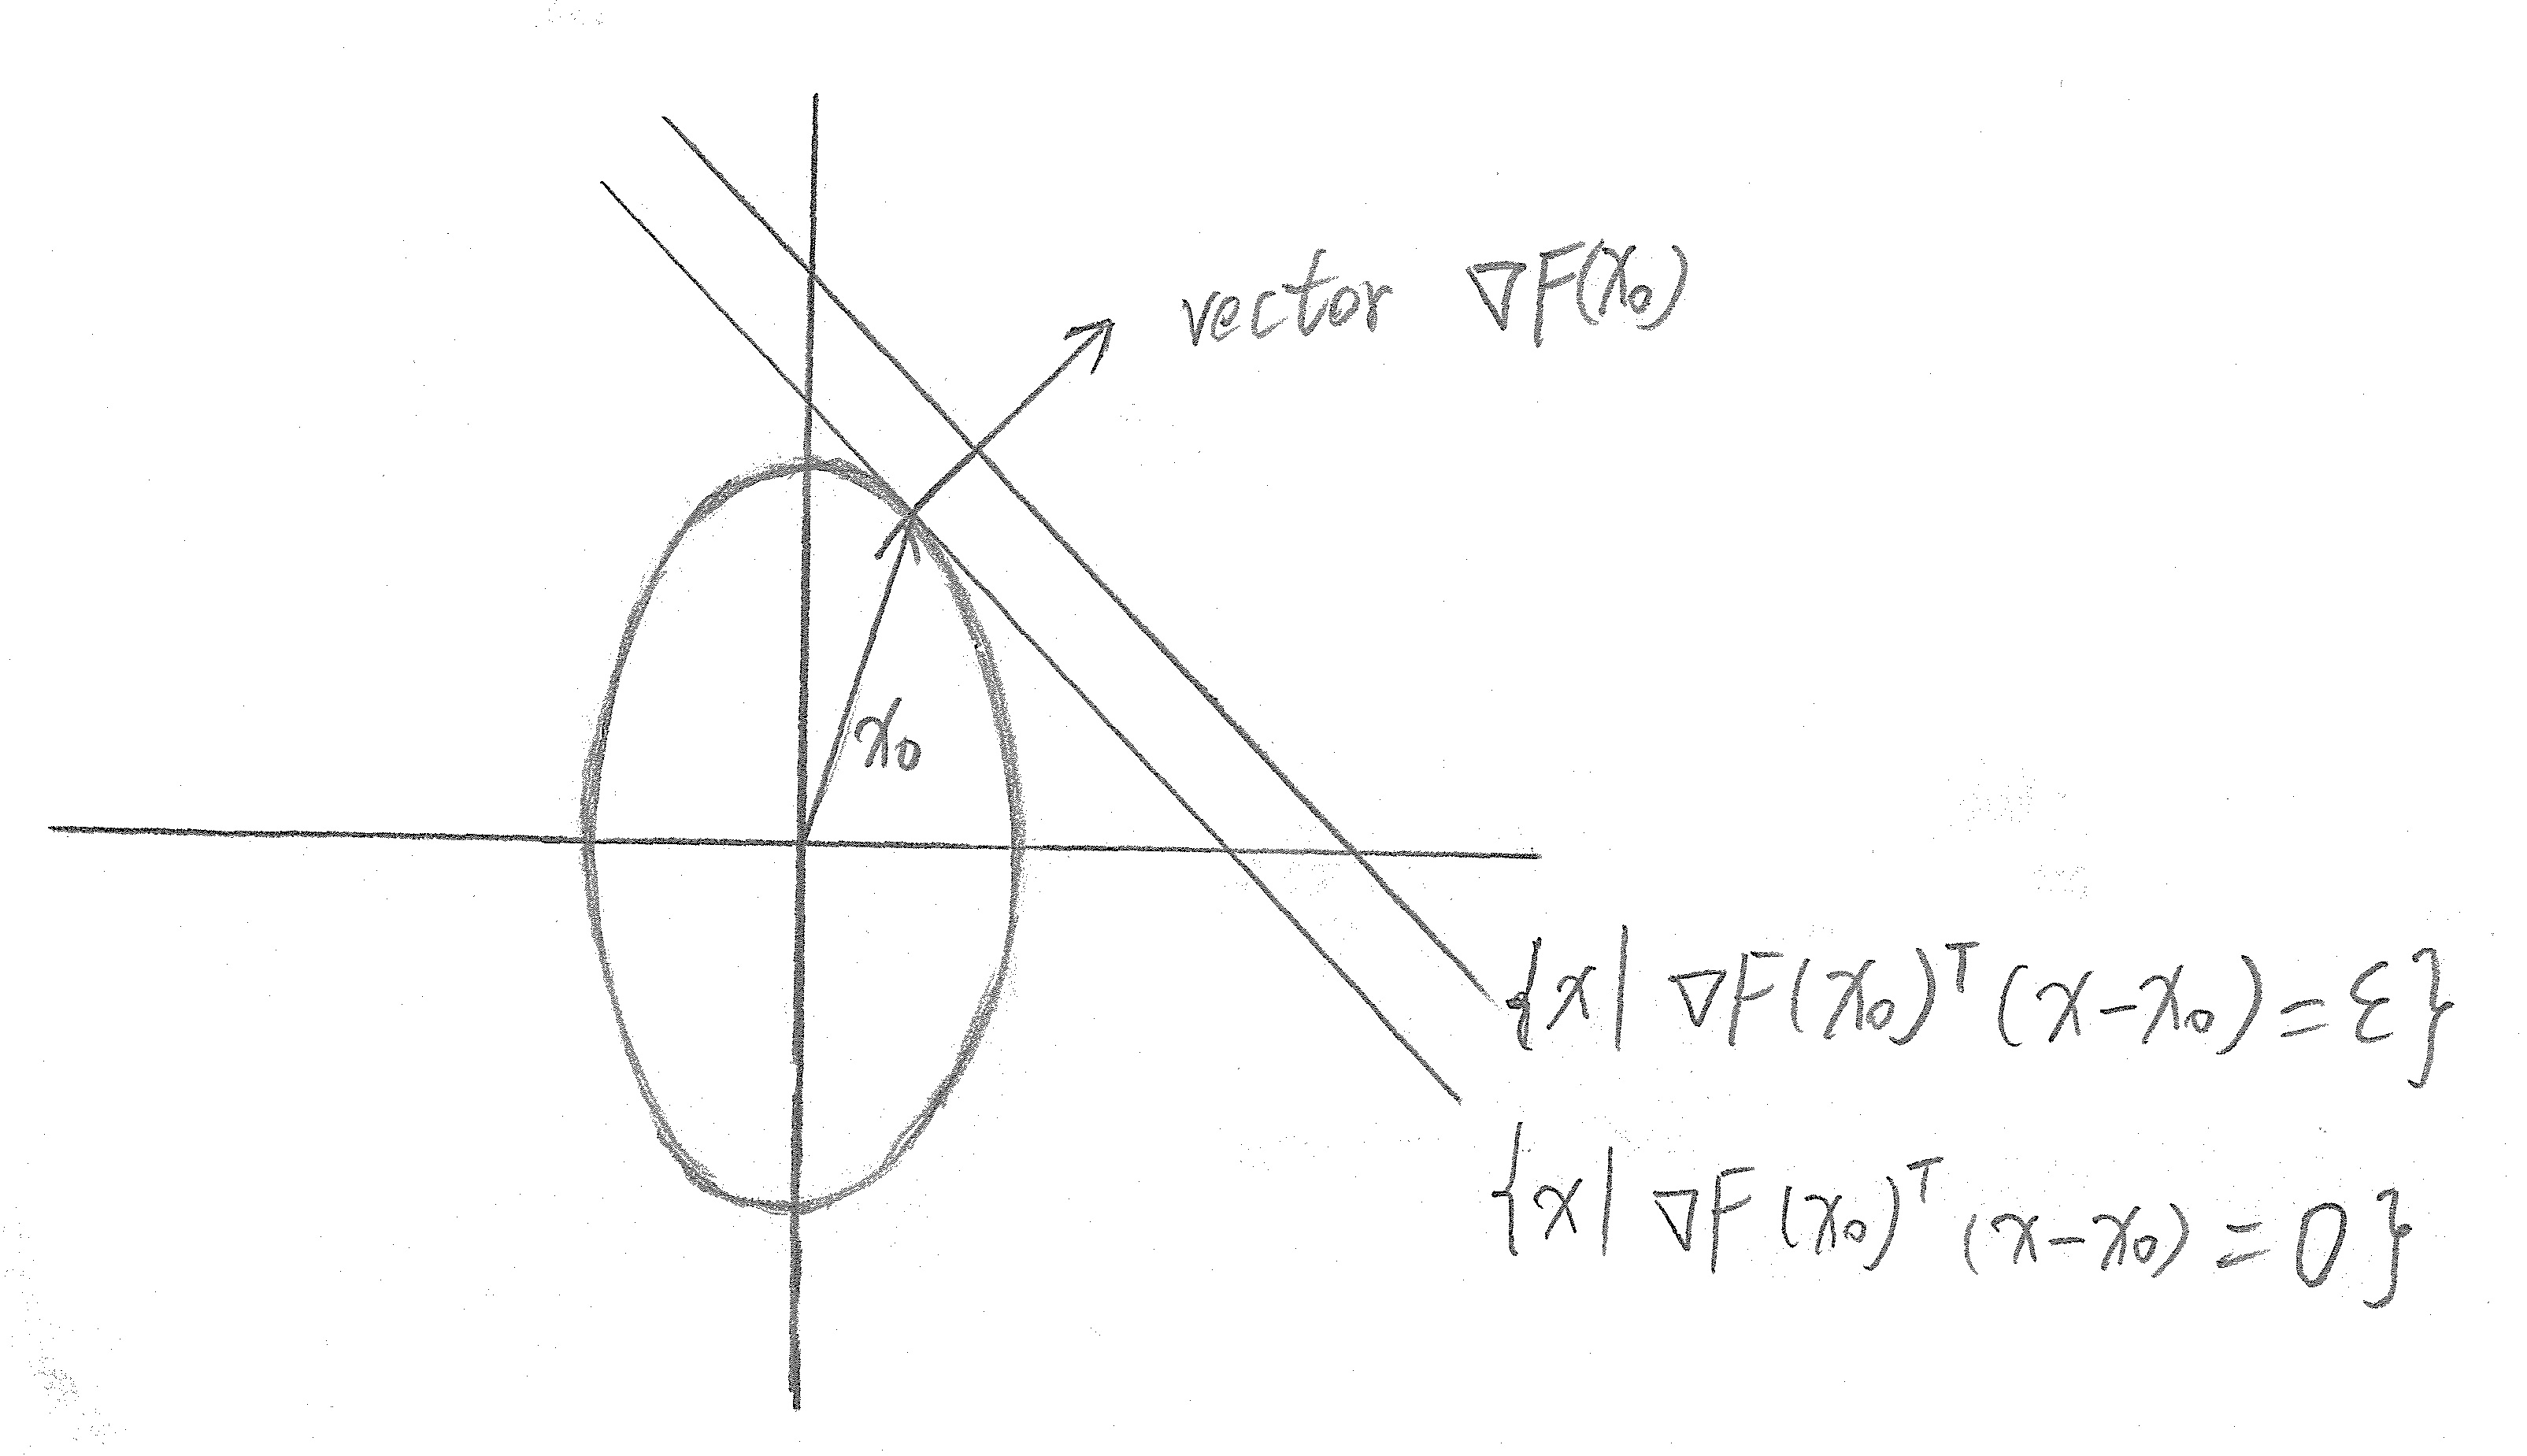
\includegraphics[width=2.1in,height=2.1in]{figures/ch02/p61.jpg}
	%\caption{This is an inserted JPG graphic} 
	%\label{fig:graph} 
\end{figure}

In general the set
\begin{align*}
&\{x | \nabla F(x_0)^{T} (x-x_0) = c\}\\
&= \{x | \nabla F(x_0)^{T} x = \nabla F(x_0)^{T} x_0 + c\} \\
&= \{x | a^{T}x = b\}
\end{align*}
which is a "hyperplane", a type of affine set. 

\vspace{0.5cm}
Observe that geometry of gradients connects to geometry of level sets. But you might think that is a bit funny. You know a Taylor sense approx is of the function $F$ not the level sets of $F$. You might also recall there is a tangent approximation involved somewhere, e.g. 

\begin{figure}
	\centering
	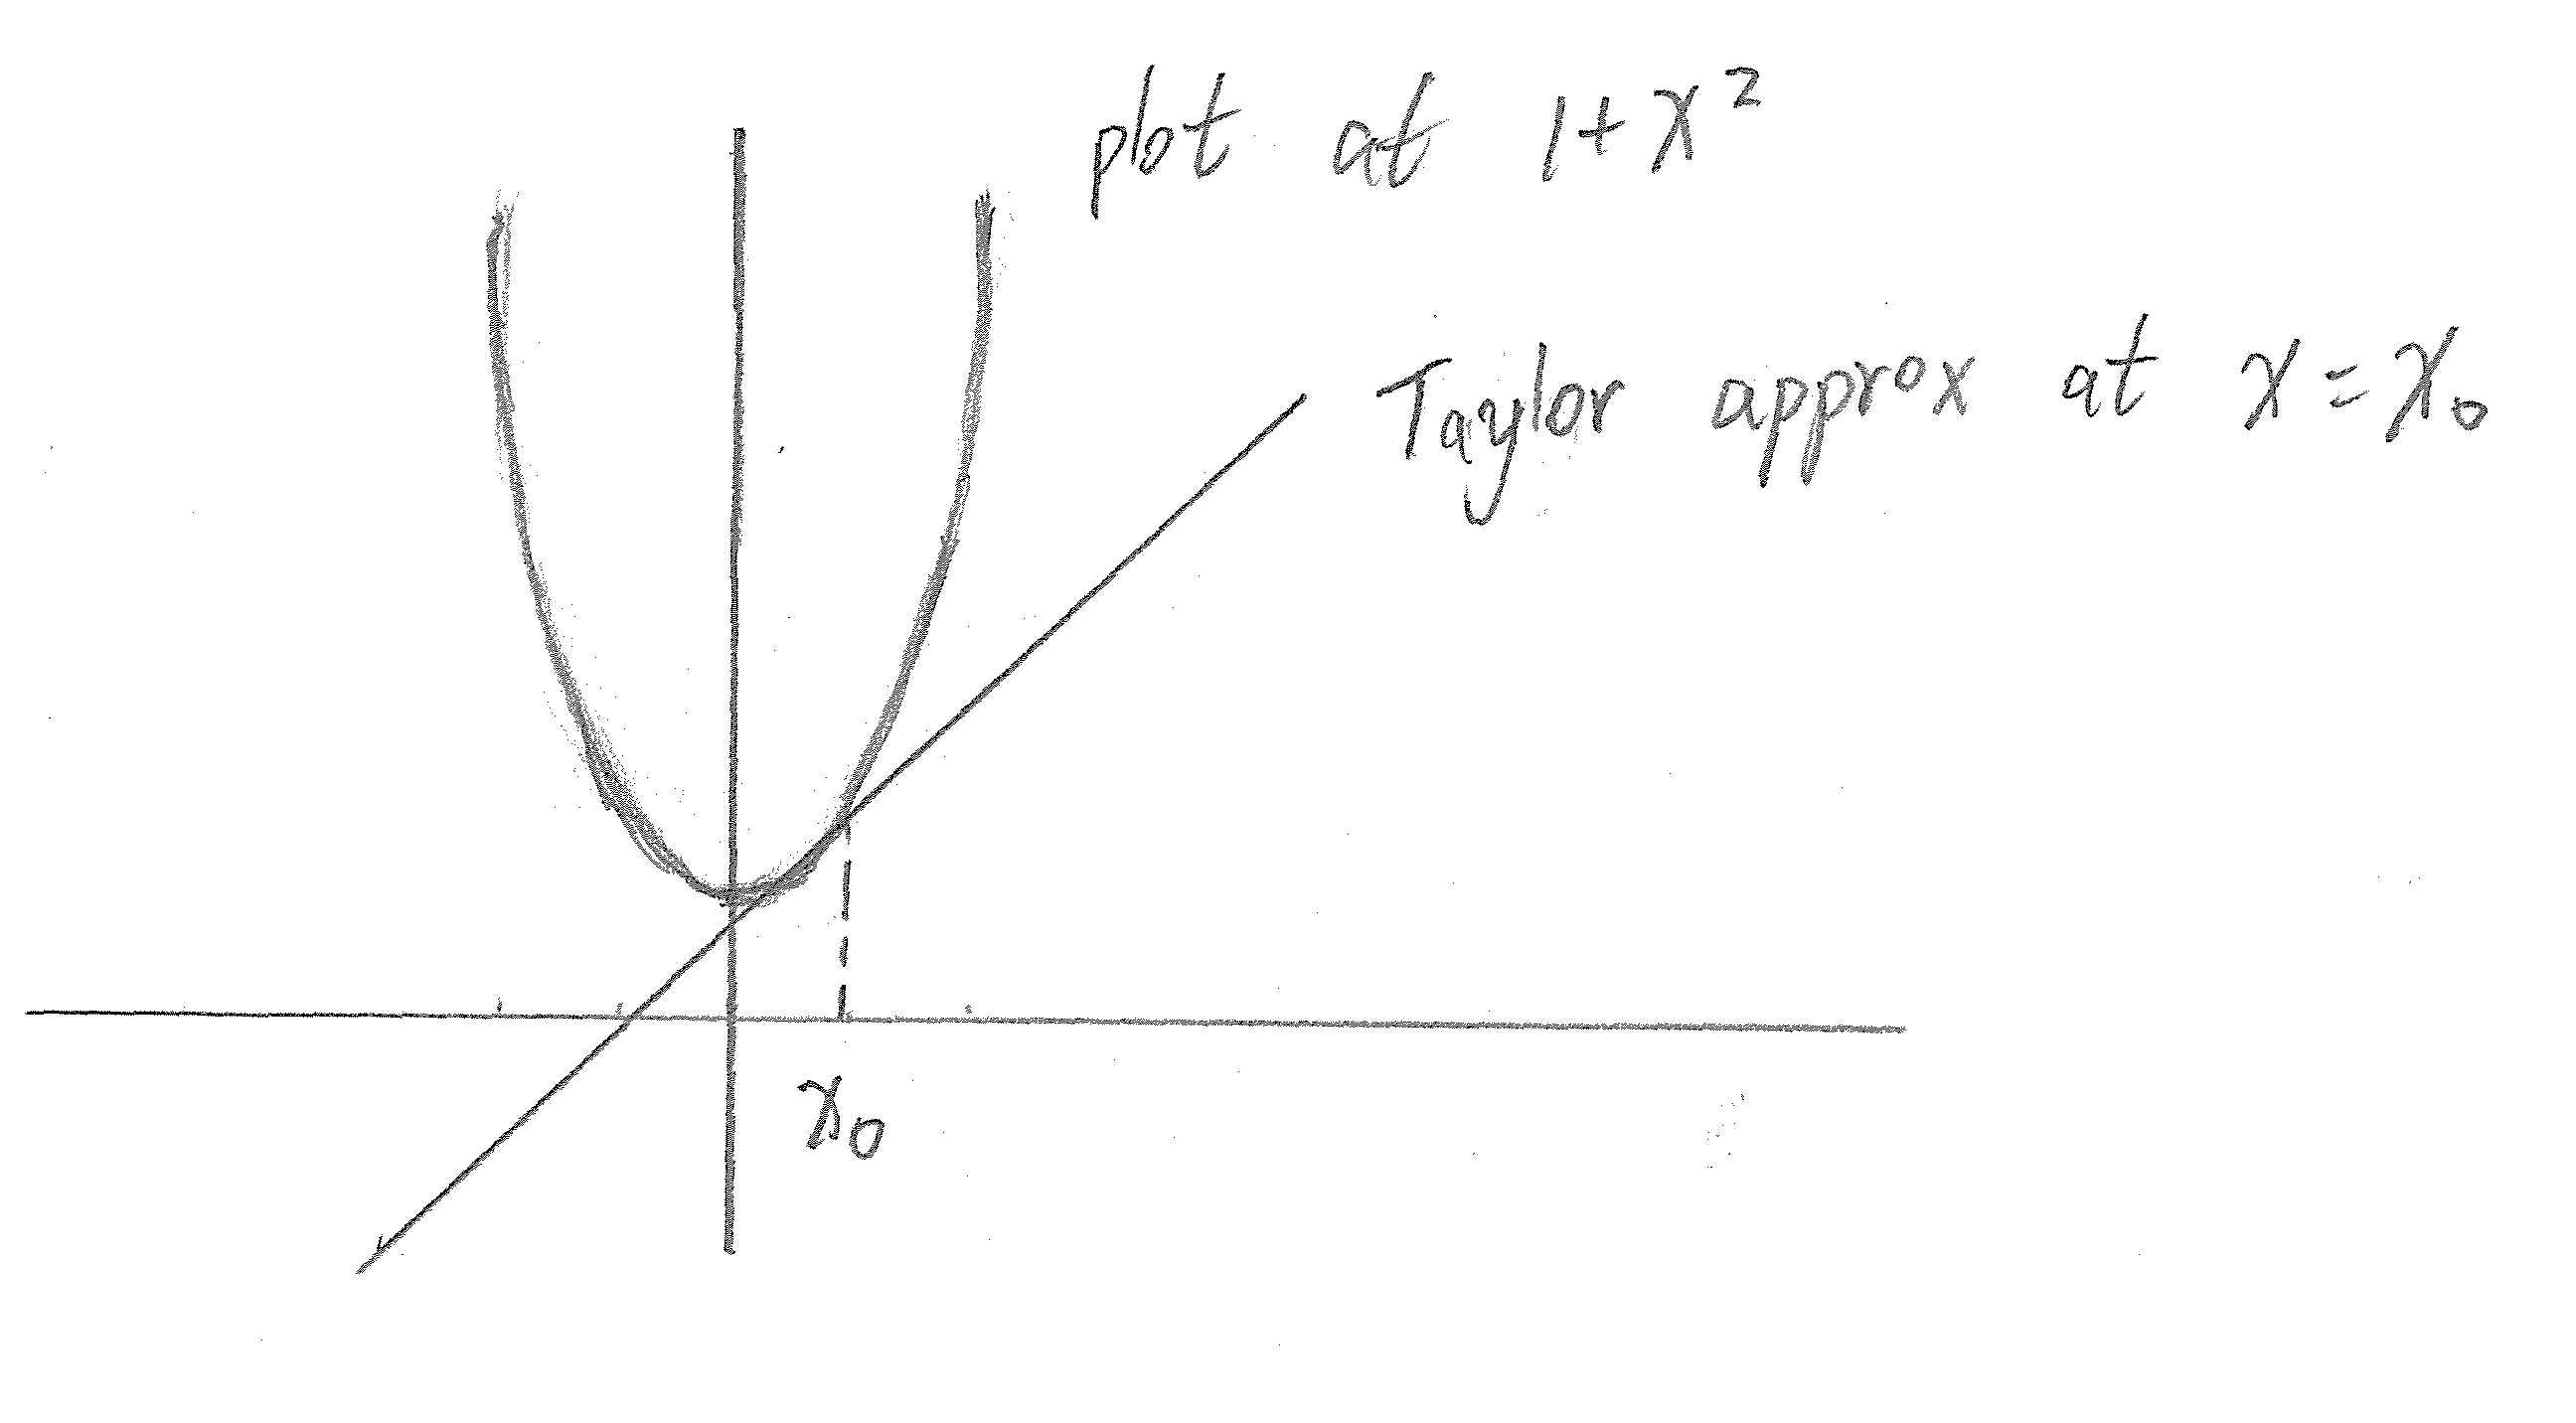
\includegraphics[width=2.1in,height=2.1in]{figures/ch02/p62.jpg}
	%\caption{This is an inserted JPG graphic} 
	%\label{fig:graph} 
\end{figure}


To develop the approximation we need to consider the plot or "graph" at the function $F$
$$\text{graph}\ F = \{(x, F(x) | x \in \mathbb{R}^n)\} \subseteq \mathbb{R}^{n+1}$$

e.g., in above example $F(x) = x^2+1$, $F \colon \mathbb{R} \to \mathbb{R}$, $s-n=1$ and plot (graph) is in $\mathbb{R}^2$.

To find the tangent approximation, we will pick a point $t$ "above". The graph, is pick some pair $(x, t)$ s.t. $t \geq F(x)$.

Use Taylor approximation above $x_0$ to approximate $F(x)$ 

\begin{figure}
	\centering
	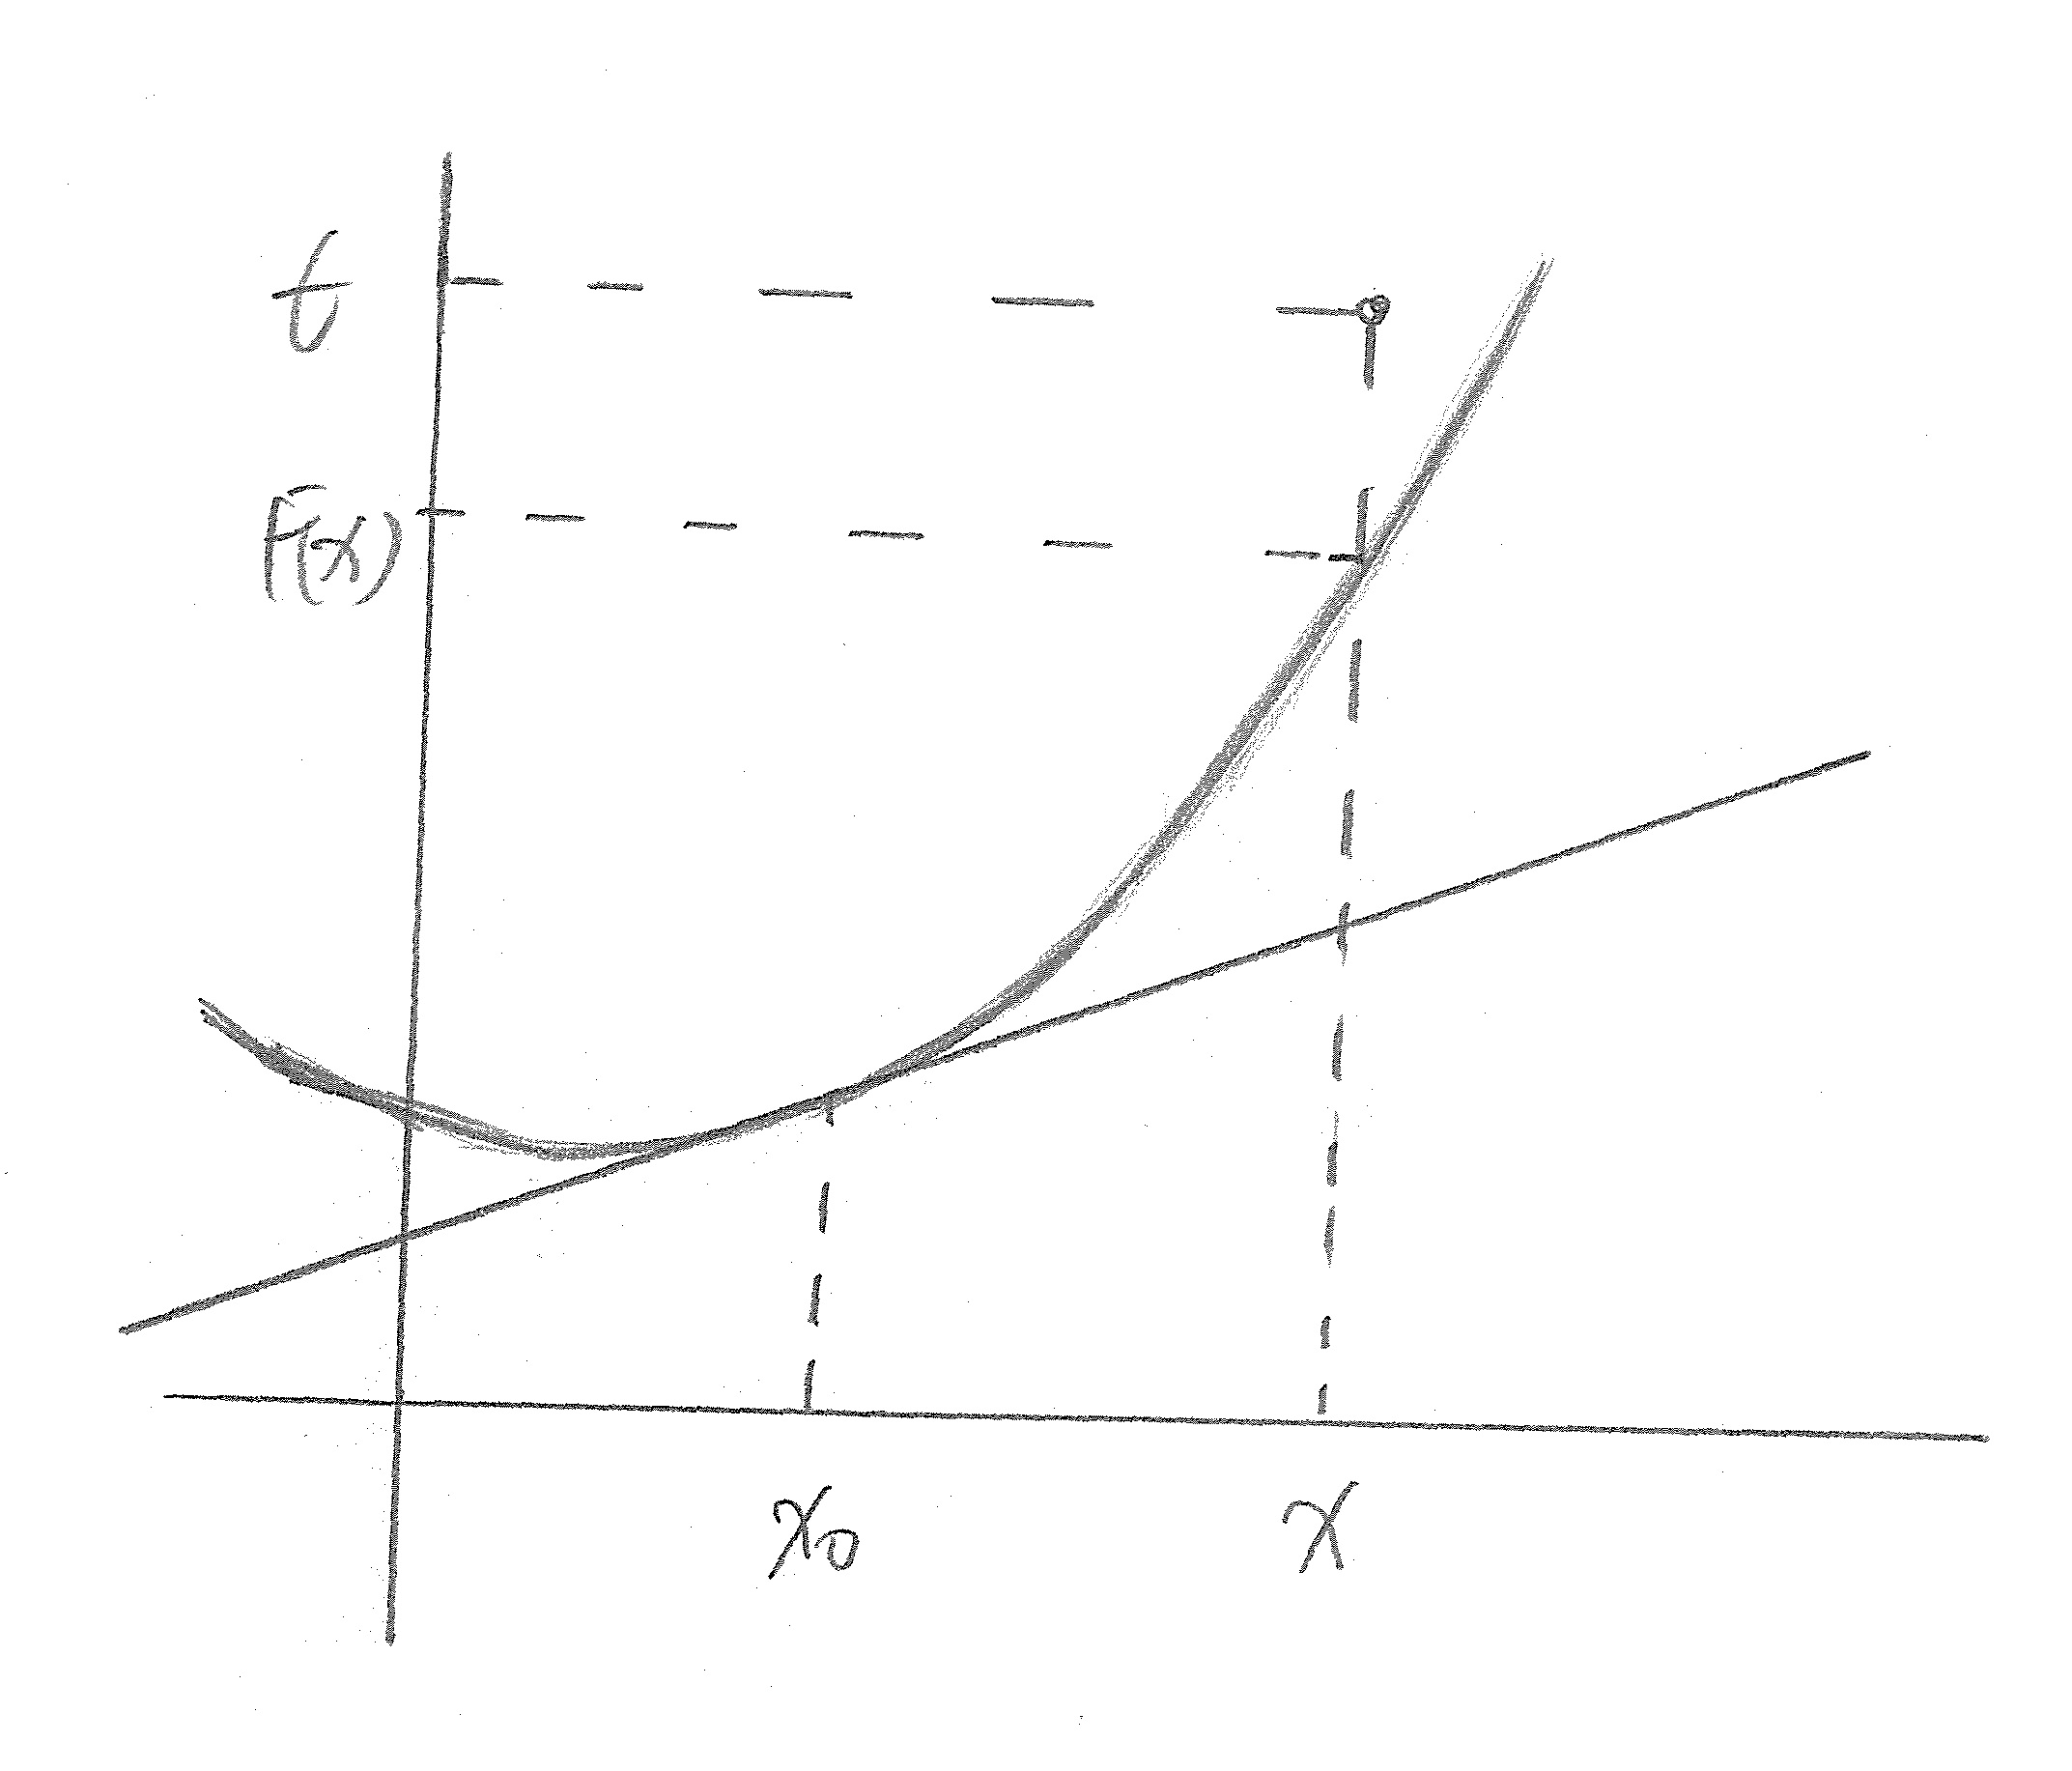
\includegraphics[width=2.1in,height=2.1in]{figures/ch02/p63.jpg}
	%\caption{This is an inserted JPG graphic} 
	%\label{fig:graph} 
\end{figure}

\vspace{0.5cm}
Recap:

(1) Pick $(x, t)$ s.t. $t \geq F(x)$
 
(2) Assume $x$ and $x_0$ are "close" so approximation is accurate.

(3) By Taylor
$F(x) = F(x_0) + \nabla F(x_0)^{T} (x-x_0) + \varepsilon(x)$

(4) By (1), $t \geq F(x) = F(x_0) + \nabla F(x_0)^{T} (x-x_0) + \varepsilon(x)$

(5) By (2) will drop the $\varepsilon(x)$ term and assume inequality doesn't flip (because $x$ and $x_0$ are sufficiently close that $\varepsilon(x)$ is sufficient small), and thus yields 
$$t \geq F(x_0) + \nabla F(x_0)^{T} (x-x_0)\qquad  (*)$$
Next, we re-arrange

(6)
\begin{align*}
0 &\geq -(t-F(x_0)) + \nabla F(x_0)^{T} (x - x_0) \\
&=\begin{bmatrix} \nabla F(x_0)^{T} -1\\ \end{bmatrix}  \begin{bmatrix} x-x_0\\ t-F(x_0)\\ \end{bmatrix} 
\end{align*}


Observe that:

(a) $(x-x_{0})\in \reals^{n}$ so vectors are in $\reals^{n+1}$.

(b) $t-F(x_{0})\in\reals$ i.e., in example plot when $n=1$ in $\reals^{2}$.

\begin{figure}
	\centering
	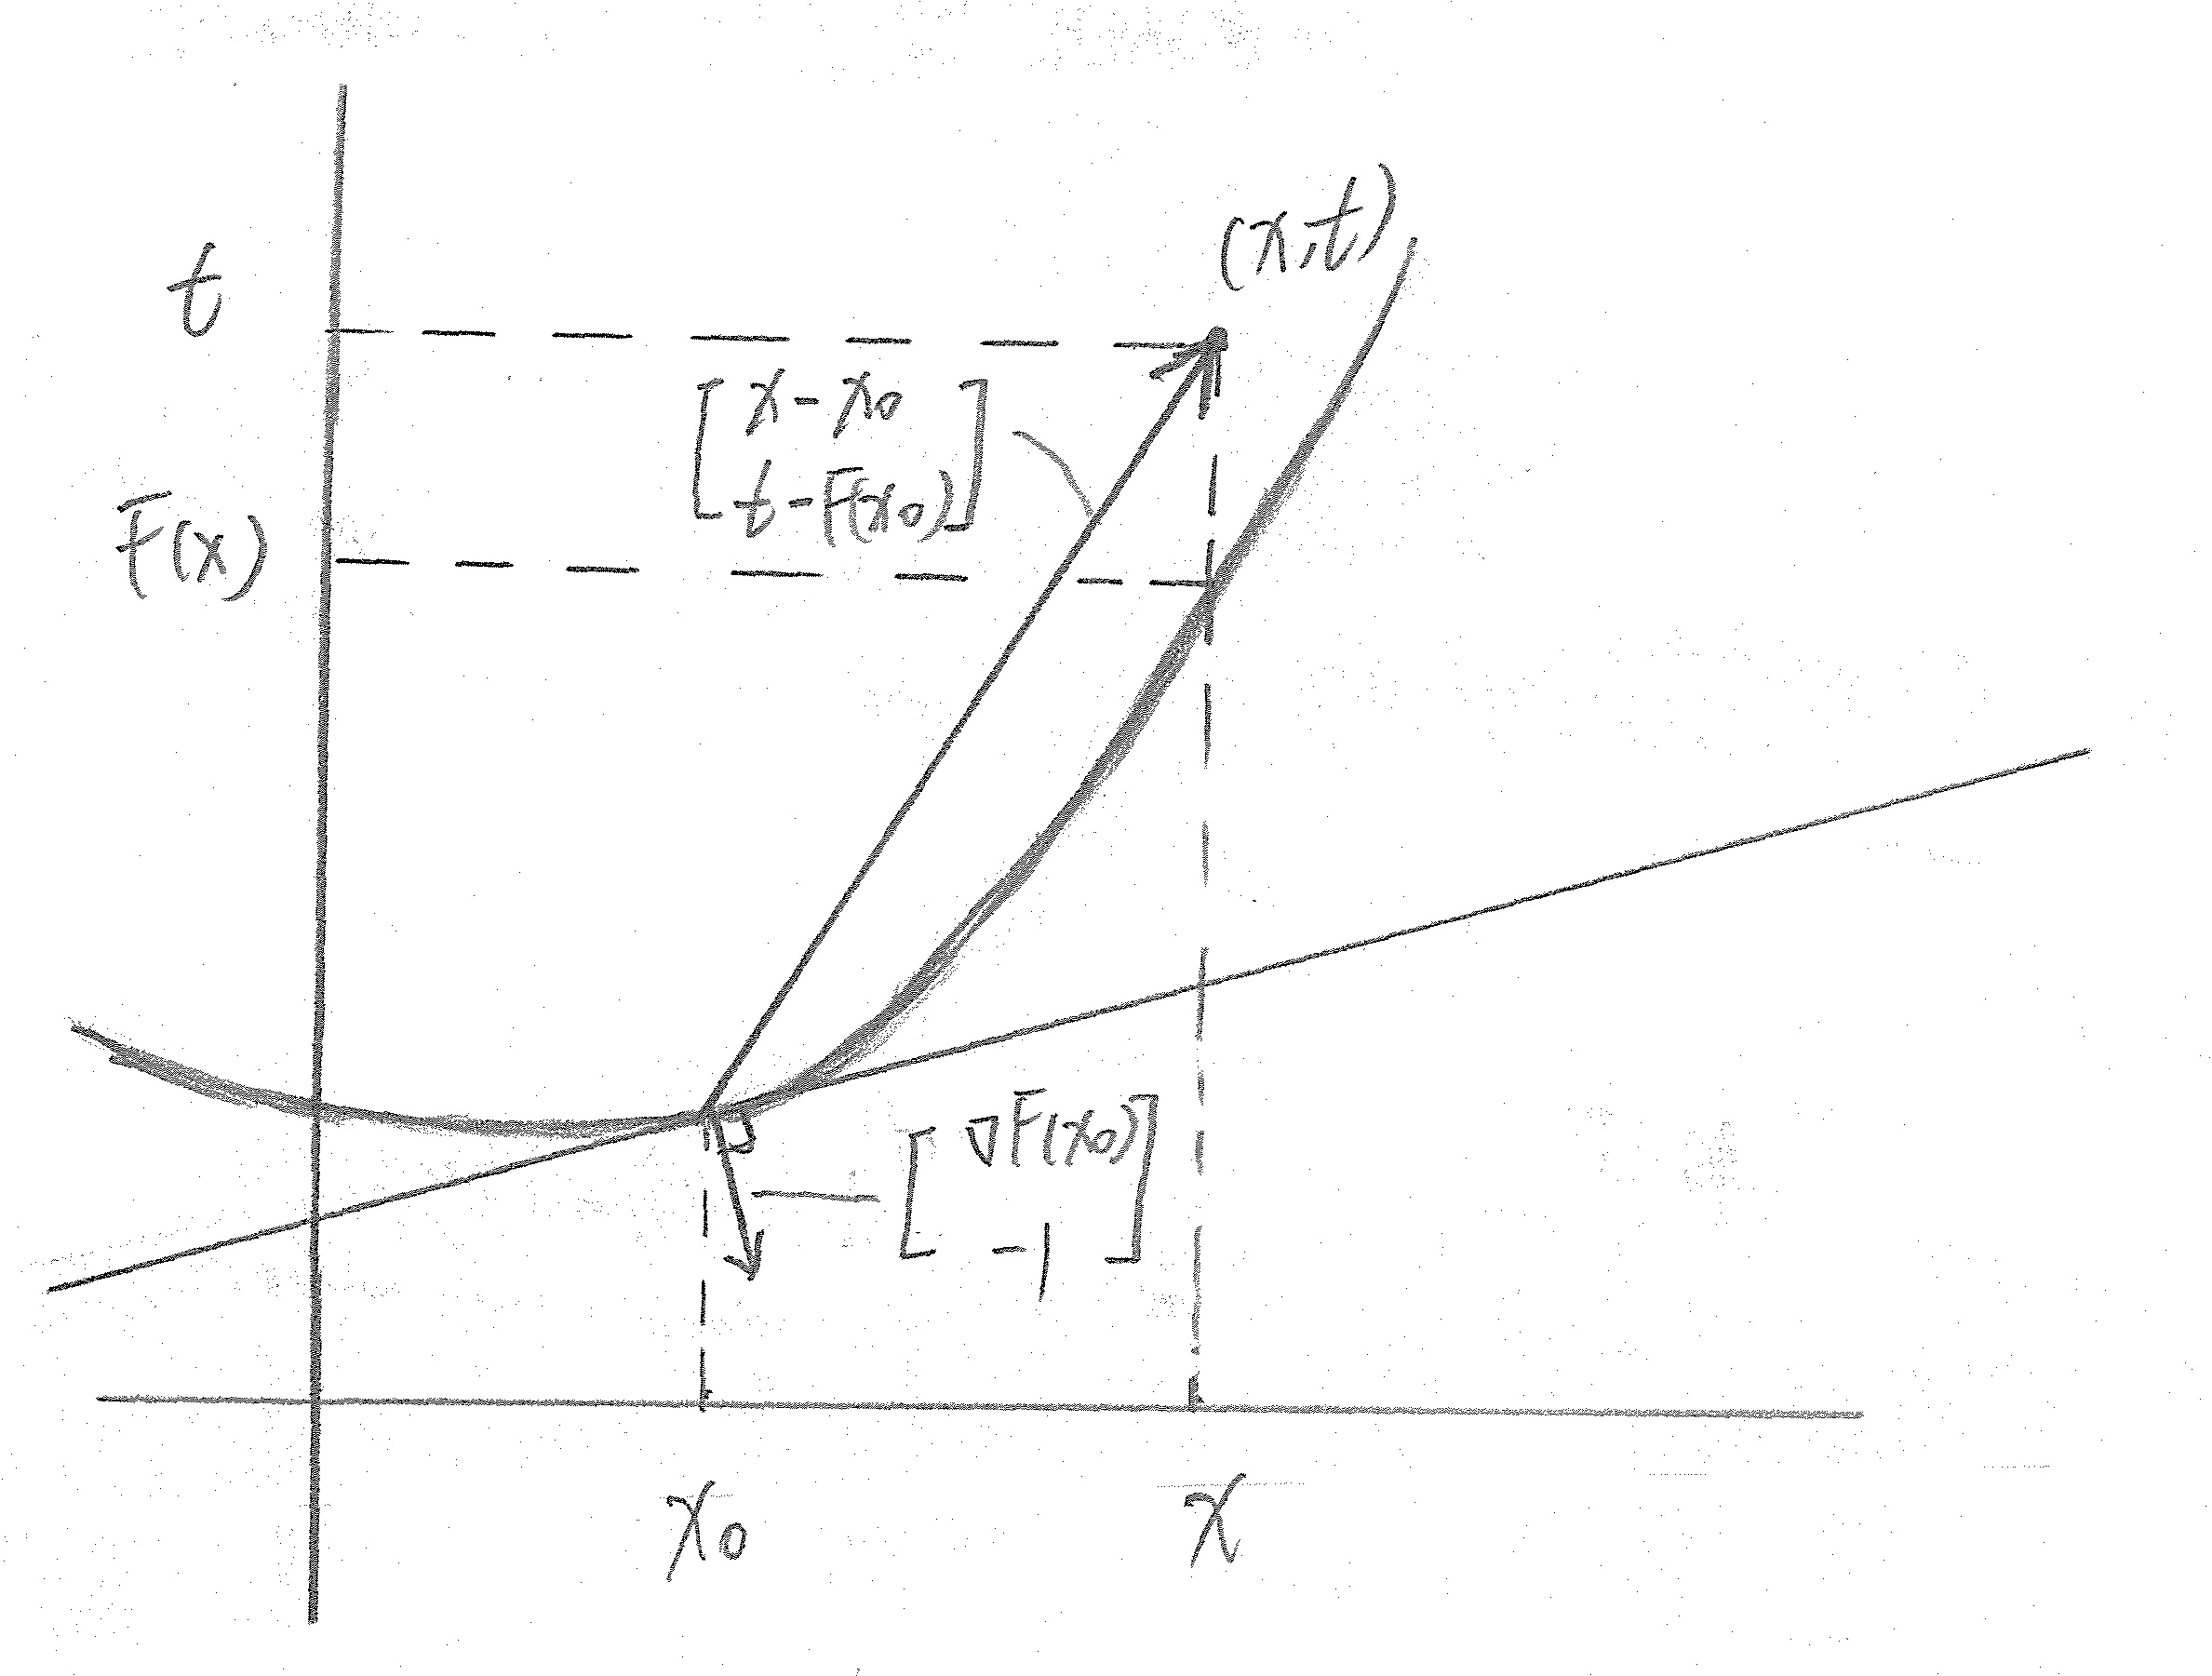
\includegraphics[width=2.1in,height=2.1in]{figures/ch02/p64.jpg}
	%\caption{This is an inserted JPG graphic} 
	%\label{fig:graph} 
\end{figure}

\vspace{0.5cm}
Now recall connection between angles and inner products.

(1). If inner product of 2 vectors is negative, then the angles is obtuse.

(2). Matches picture.

What about vectors when this inner product = 0 ? That is
$$\{u\in\reals^{n+1}|\langle u, [\nabla F(x_{0}) , -1]^{\trans}\rangle=0\}$$

writing $u=[x-x_{0}, t-F(x_{0}]^{\trans}$ and no longer require $t\geq F(x)$.

The condition becomes
$$
\left[
\begin{array}{c} 
	x-x_{0}\\
	t-F(x_{0})
\end{array}
\right]^{\trans}  
\left[
\begin{array}{c} 
\nabla F(x_{0})\\
-1
\end{array}
\right]
=
0
$$

So we recognize the set defines a hyperplane in $\reals^{n+1}$,
$$\mathcal{H}=\left\{\left[
\begin{array}{c} 
	x \\
    t
\end{array}
\right]  
\middle|      
\left[
\begin{array}{cc} 
x^{\trans}&t
\end{array}
\right]  
\left[
\begin{array}{c} 
\nabla F(x_{0}) \\
-1
\end{array}
\right]  
=
\left[
\begin{array}{cc} 
x_{0}^{\trans}&F(x_{0})
\end{array}
\right]  
\left[
\begin{array}{c} 
	\nabla F(x_{0}) \\
	-1
\end{array}
\right]  
\right\}$$
This is called a "supporting hyperplane" of the epigraph.

Finally, let's look at Taylor approximation one last time (1st order approximation), and recall the geometric interpretation of each of the pieces:
\begin{align*}
F(x)&\approx F(x_{0})+ \nabla F(x_{0})^{\trans}(x-x_{0})\\
&=F(x_{0})+\Vert\nabla F(x_{0})\Vert \Vert x-x_{0}\Vert \left< \frac{\nabla F(x_{0})}{\Vert\nabla F(x_{0})\Vert},\frac{x-x_{0}}{\Vert x-x_{0}\Vert}\right>\\
&=\text{bias + steepness $\times$ distance $\times$ angle }
\end{align*}
























 








